%% main_ppgee_ufu.tex v1.0, Milton Miranda Neto
% adaptado de modeloABNT2.tex, v1.0 LabCG 
% ------------------------------------------------------------------------
% eesc: Modelo de Trabalho Acadêmico (tese de doutorado, dissertação de
% mestrado e trabalhos monográficos em geral) em conformidade com 
% ABNT NBR 14724:2011. 
% ------------------------------------------------------------------------
% Atualizações.
% 15/10/2018 - Adaptação para a FEELT-UFU.

% ------------------------------------------------------------------------
% Opções:
%   tesedr:     Formata documento para tese de doutorado
%   qualidr:    Formata documento para qualificação de doutorado
%   dissertmst: Formata documento para dissertação de mestrado
%   qualimst:   Formata documento para qualificação de mestrado
% ------------------------------------------------------------------------
\documentclass[tesedr]{ppgee}
%Não altere o comando seguinte. O título de seu trabalho será especificado mais adiante.
\title{Template de Monografia FEELT-UFU} % Este título é sobrescrito pelo comando \titulo{} abaixo

% ---
% PACOTES
% ---

% ---
% Pacotes fundamentais 
% ---
\usepackage{cmap}                % Mapear caracteres especiais no PDF (bom para busca e cópia)
\usepackage{lmodern}             % Usa a fonte Latin Modern (boa qualidade com T1)
\usepackage{makeidx}             % Cria o indice remissivo (se for utilizá-lo)
\usepackage{lastpage}            % Usado pela Ficha catalográfica para contar o total de páginas
\usepackage{indentfirst}         % Indenta o primeiro parágrafo de cada seção.
\usepackage{nomencl}             % Para lista de símbolos (se for utilizá-la)
% \usepackage{graphicx}          % REMOVIDO - Já carregado por ppgee.cls (\RequirePackage{calc,graphicx})
\usepackage{textcomp}            % Para símbolos adicionais de texto
\usepackage{amsmath,amssymb}     % cases, align, \text{} e símbolos matemáticos
\usepackage{bm}                  % negrito matemático (\bm)
\usepackage{booktabs}            % regras de tabela (\toprule/\midrule/\bottomrule)
\usepackage{multirow}            % células que ocupam várias linhas

% \usepackage{subfigure}         % REMOVIDO - Pacote obsoleto. 
                                 % A classe ppgee.cls usa \newsubfloat{figure}, que é um comando
                                 % tipicamente do pacote 'subfig'. Se precisar de subfiguras, 
                                 % considere usar \usepackage{subfig} ou \usepackage{subcaption} 
                                 % e verifique a compatibilidade ou ajuste \newsubfloat se necessário.
                                 % Para uma simples remoção de obsoleto, apenas removemos.

% Pacotes essenciais para algoritmos
% \usepackage{algorithm}         % REMOVIDO/COMENTADO - Já carregado por ppgee.cls
% \usepackage{algpseudocode}     % REMOVIDO/COMENTADO - Conflitante com o 'algorithmic' de ppgee.cls
% \usepackage{algorithmic}       % REMOVIDO/COMENTADO - Já carregado por ppgee.cls
% \usepackage{algorithmicx}      % REMOVIDO/COMENTADO - Conflitante e/ou redundante

% ---
% Pacotes adicionais, usados apenas no âmbito do Modelo eesc (ou do seu trabalho)
% ---
\usepackage{lipsum}              % Para geração de texto de preenchimento (remover na versão final)
\usepackage[printonlyused]{acronym} % Para lista de acrônimos (se for utilizá-la)
\usepackage[table]{xcolor}       % Para cores, especialmente em tabelas. ppgee.cls carrega 'color',
                                 % mas 'xcolor' é mais poderoso e geralmente compatível.

% ---
% Pacotes que idealmente são carregados por último
% ---
\usepackage{hyperref}            % Controla links e informações do PDF. Movido para o final.
                                 % A classe ppgee.cls já faz um \hypersetup.

% ---
% Informações de dados para CAPA e FOLHA DE ROSTO (mantido como no seu original)
% ---
% ============================================================================
% PENDENTE: TÍTULO. O título abaixo é o da QUALIFICAÇÃO e promete "Fusão
% Sensorial Heterogênea" e "Aprendizado por Reforço" -- dois componentes que o
% sistema avaliado nos Cap. 4-6 NÃO entrega (a percepção é abstraída em eventos
% e a atualização de valor não seleciona as ações executadas; ver Seção
% \ref{sec:prop-atualizacao} e o ajuste de escopo na Seção
% \ref{sec:conc-limitacoes}). Os revisores da IEEE Access exigiram a retirada
% dessas alegações do artigo.
% Título alinhado ao entregue, para decisão com o orientador:
%   Arquitetura Deliberativo-Reativa de Duas Camadas com Camada de
%   Atração--Repulsão Acionada por Limiar para Inspeção de Subestações Elétricas
% Se trocar: atualizar também capa, ficha catalográfica, folha de aprovação e os
% formulários SEI em docs/documentos-banca/.
% ============================================================================
%% Titulo definido em 12/11/2026. Mantem a espinha do titulo do artigo aceito
%% (IEEE Access, Access-2026-33687) para que a relacao seja imediata, e acrescenta
%% no subtitulo o que so a tese entrega: o estudo de atribuicao de efeitos a
%% mecanismos, que e o que o objetivo geral promete. O titulo anterior prometia
%% fusao sensorial heterogenea e aprendizado por reforco, que os resultados mostraram
%% nao governarem o comportamento executado -- ver a subsecao "Delimitacao de
%% Escopo" na introducao. DEVE BATER, letra por letra, com o campo 1.10 da
%% solicitacao de banca (SEI 7735815) e o 1.8 da ficha de indicadores (SEI 7481935).
\titulo{Arquitetura Deliberativo-Reativa de Duas Camadas para Inspeção de Subestações Elétricas: Campo de Atração--Repulsão Acionado por Limiar e Atribuição Experimental de Efeitos a Mecanismos}{A Two-Layer Deliberative--Reactive Architecture for Substation Inspection: Threshold-Triggered Attraction--Repulsion Field and Experimental Attribution of Effects to Mechanisms}
\autor{Milton Miranda Neto}{Miranda Neto, Milton}
\local{Uberlândia}
\data{2026}
\areaconcentracao{Engenharia Elétrica}
\orientador{Alexandre Cardoso}
\coorientador{Edgard Afonso Lamounier Junior}
% ---

% ---
% compila o indice (mantido como no seu original)
% ---
\makeindex
% ---

% ---
% Compila a lista de abreviaturas e siglas (mantido como no seu original)
% ---
\makenomenclature % Garanta que este comando esteja presente se usar \printnomenclature
% ---

% ---
% Inserir ficha catalográfica
%
% Caso o comando \inserirfichacatalografica seja definido, a %ficha catalográfica
% será inserida atrás da folha de rosto. Caso contrário a página será deixada em
% branco.
%
% CUIDADO: Esta opção deve ser preenchida antes do comando \maketitle
% ---
%entre em contato com a biblioteca para obter a sua ficha catalográfica em arquivo pdf. Essa %folha só será inserida no documento após a sua defesa.

%\inserirfichacatalografica{fichaCatalografica.pdf}
% ---

% ---
% Inserir folha de aprovação
%
% Caso o comando \inserirfolhaaprovacao seja definido, a a folha de aprovação
% será inserida. Além disso, conforme Resolução CoPGr 5890, as informações 
% de rodapé são inseridas apropriadamente na folha de rosto.
%
% CUIDADO: Esta opção deve ser preenchida antes do comando \maketitle
% ---
% baseie-se no modelo desse documento e gere a sua folha de %rosto em arquivo pdf.

%\inserirfolhaaprovacao{folhaAprovacao.pdf}
% ---

% ----
% Início do documento
% ----

\begin{document}

% ----------------------------------------------------------
% ELEMENTOS PRÉ-TEXTUAIS
% ----------------------------------------------------------
\pretextual

% ---
% Insere Capa, Folha de rosto, Ficha catalográfica (se inserida)
% e folha de aprovação (se inserida).
% ---
\maketitle

% ---
% Dedicatória
% ---
\imprimirdedicatoria{Dedico este trabalho à minha família, fonte constante de apoio e inspiração.}
% ---

% ---
% Agradecimentos
% ---
\imprimiragradecimentos{

Agradeço primeiramente a minha família, pelo apoio constante, compreensão e incentivo em todos os momentos.

Ao meu orientador, Alexandre Cardoso, pelo suporte, confiança e inestimada orientação ao longo deste trabalho.

Aos colegas e amigos que contribuíram direta ou indiretamente com palavras de ânimo e sugestões valiosas.

Por fim, agradeço ao Programa de Pós-Graduação em Engenharia Elétrica da Universidade Federal de Uberlândia, em especial aos professores e a querida Andressa, secretária do programa de Pós-Graduação, por toda a sua dedicação e paciência.

Muito Obrigado a Todos!                       

“UP THE IRONS!” 

}
% ---

% ---
% Epígrafe
% ---
\imprimirepigrafe{
		``Don't waste your time always searching for those wasted years. Face up, make your stand And realize you're living in the golden years.''\\
		(Iron Maiden)
}
% ---

% ---
% RESUMO e ABSTRACT
% ---

% Resumo em português - as palavras entre chaves são as palavras-chave do trbalho
\begin{resumo}{Navegação autônoma; Arquitetura deliberativo-reativa; Campo de atração--repulsão; Inspeção de subestações; ROS~2; Nav2.}

Robôs de inspeção de subestações tipicamente seguem uma patrulha fixa, sem adaptar o
percurso ao que percebem, enquanto um controlador puramente reativo responde apenas a
estímulos já dentro do alcance sensorial. Esta tese faz a ponte entre esses dois
regimes com uma arquitetura de duas camadas: uma patrulha deliberativa de
\emph{sensoriamento ativo} (ROS~2, Nav2, MPPI) conduz os sensores até onde eventos
possam ocorrer, e uma camada reativa converte a saliência sensorial em um campo de
atração/repulsão que aciona, por limiar, um controlador de estados finitos
responsável por aproximar o robô de anomalias e afastá-lo de riscos, sob uma regra
categórica que faz o canal de risco governar sempre que um risco seja elegível. A
arquitetura é avaliada em subestação simulada (Gazebo Fortress) contra uma patrulha
fixa, uma linha de base de campo potencial artificial e uma heurística genérica de
detectar--selecionar--desviar--retornar executada sobre o \emph{mesmo} controlador
Nav2/MPPI, o que isola o campo do mero ato de desviar. Três achados decorrem. Primeiro,
sobre um risco \emph{estático} na rota de patrulha, uma patrulha fixa portando a mesma
zona de exclusão disparada por detecção, mas sem supervisor reativo, alcançou
afastamento mínimo sem diferença estatisticamente detectável da ablação que retém a
inspeção reativa ($1{,}73$ contra $1{,}71$~m de mediana): o benefício de segurança
nesse caso é atribuível à zona de exclusão deliberativa, e não à ponderação reativa, e
o que a camada reativa acrescenta são as inspeções ($3$ contra $0$ de $3$). Segundo,
substituir a saliência pela proximidade não produziu diferença detectável em cenário
algum, ao passo que substituir o campo com limiar por detecção bruta --- o que também
remove a persistência temporal do canal de risco --- reduz o afastamento à metade
quando um risco é colocalizado com uma anomalia mais saliente ($4{,}84$ contra
$2{,}23$~m) e atrasa a inspeção prioritária em cerca de $105$~s. Terceiro, essa
precedência tem custo: um risco marginalmente elegível suprime a atração por cerca de
$70$~s e abre mão de uma de quatro inspeções. A completude de inspeção degrada-se sob
ruído alto de percepção e sob aglomeração densa, e o número de execuções por
configuração limita, mas não elimina, o risco de entrada em região de contato. A
percepção é abstraída em eventos-oráculo e a transformada de localização é fixa, de
modo que os resultados falam da lógica de decisão, e não de um sistema pronto para
implantação. Código, mundo simulado, dados e \textit{scripts} são publicados.

\end{resumo}


% Resumo em inglês
\begin{abstract}{Autonomous navigation; Deliberative--reactive architecture; Attraction--repulsion field; Substation inspection; ROS~2; Nav2.}

Substation-inspection robots typically follow a fixed patrol without adapting to what
they sense, while a purely reactive controller responds only to stimuli already within
sensor range. This thesis bridges these regimes with a two-layer architecture: a
deliberative \emph{active-sensing} patrol (ROS~2, Nav2, MPPI) carries the sensors to
where events may occur, and a reactive layer turns sensory saliency into an
attraction/repulsion field driving a threshold-triggered finite-state controller that
approaches anomalies and retreats from hazards, under a categorical rule that makes the
hazard channel govern whenever a hazard is eligible. The architecture is evaluated in a
simulated substation (Gazebo Fortress) against a fixed patrol, a potential-field
baseline and a generic detect--select--deviate--return heuristic on the \emph{same}
Nav2/MPPI controller, which isolates the field from the act of deviating. Three findings
follow. First, on a \emph{static} hazard on the patrol route, a fixed patrol carrying
the same detection-triggered keep-out but no reactive supervisor reached a minimum
clearance with no statistically detectable difference from the ablation that keeps the
reactive inspection ($1.73$ vs.\ $1.71$~m median): the safety benefit here is
attributable to the deliberative keep-out, not to the reactive weighting, and what the
reactive layer adds is the inspections ($3$ vs.\ $0$ of $3$). Second, replacing saliency
by proximity produced no detectable difference in any scenario, whereas replacing the
thresholded field by raw detection---which also removes the hazard channel's temporal
persistence---halves the clearance when a hazard is co-located with a more salient
anomaly ($4.84$ vs.\ $2.23$~m) and delays the priority inspection by ${\approx}105$~s.
Third, that precedence has a cost: a marginally eligible hazard suppresses attraction
for ${\approx}70$~s and forfeits one of four inspections. Inspection completeness
degrades under high perception noise and under dense clustering, and the number of runs
per configuration bounds rather than excludes the risk of entering a contact region.
Perception is abstracted to oracle events and the localization transform is fixed, so
the results speak to the decision logic, not to a deployable system. Code, world, data
and scripts are released.

\end{abstract}
% ---

% ---
% inserir lista de ilustrações
% ---
\listailustracoes
% ---

% ---
% inserir lista de tabelas
% ---
\listatabelas
% ---

% ---
% inserir lista de abreviaturas e siglas
% ---
\listasiglas{abrev/Abreviaturas}
% ---

% ---
% inserir o sumario
% ---
\sumario
% ---

% ----------------------------------------------------------
% ELEMENTOS TEXTUAIS
% ----------------------------------------------------------
\mainmatter

% ----------------------------------------------------------
% Introdução
% ----------------------------------------------------------
\chapter[Introdução]{Introdução}
\label{cap:introducao}

\section{Contextualização do Tema}
A manutenção e operação eficiente de infraestruturas críticas, como subestações de energia elétrica, são fundamentais para garantir a estabilidade e a segurança do fornecimento de energia à sociedade \cite{suitelec2023}. Essas instalações, frequentemente complexas e localizadas em áreas remotas ou de difícil acesso, demandam inspeções regulares para identificar potenciais falhas, desgastes ou condições anormais que possam comprometer seu funcionamento ou representar riscos. Tradicionalmente, essas inspeções são realizadas por equipes humanas, um processo que, embora essencial, pode ser custoso, demorado, sujeito a erros humanos e, em certos casos, expor os trabalhadores a ambientes perigosos \cite{Li2025SafetyRisk}. A \autoref{fig:contextualizacao} sugere o uso de um robô quadrúpede realizando uma inspeção em uma subestação de energia elétrica.

\begin{figure}[h!]
    \centering
    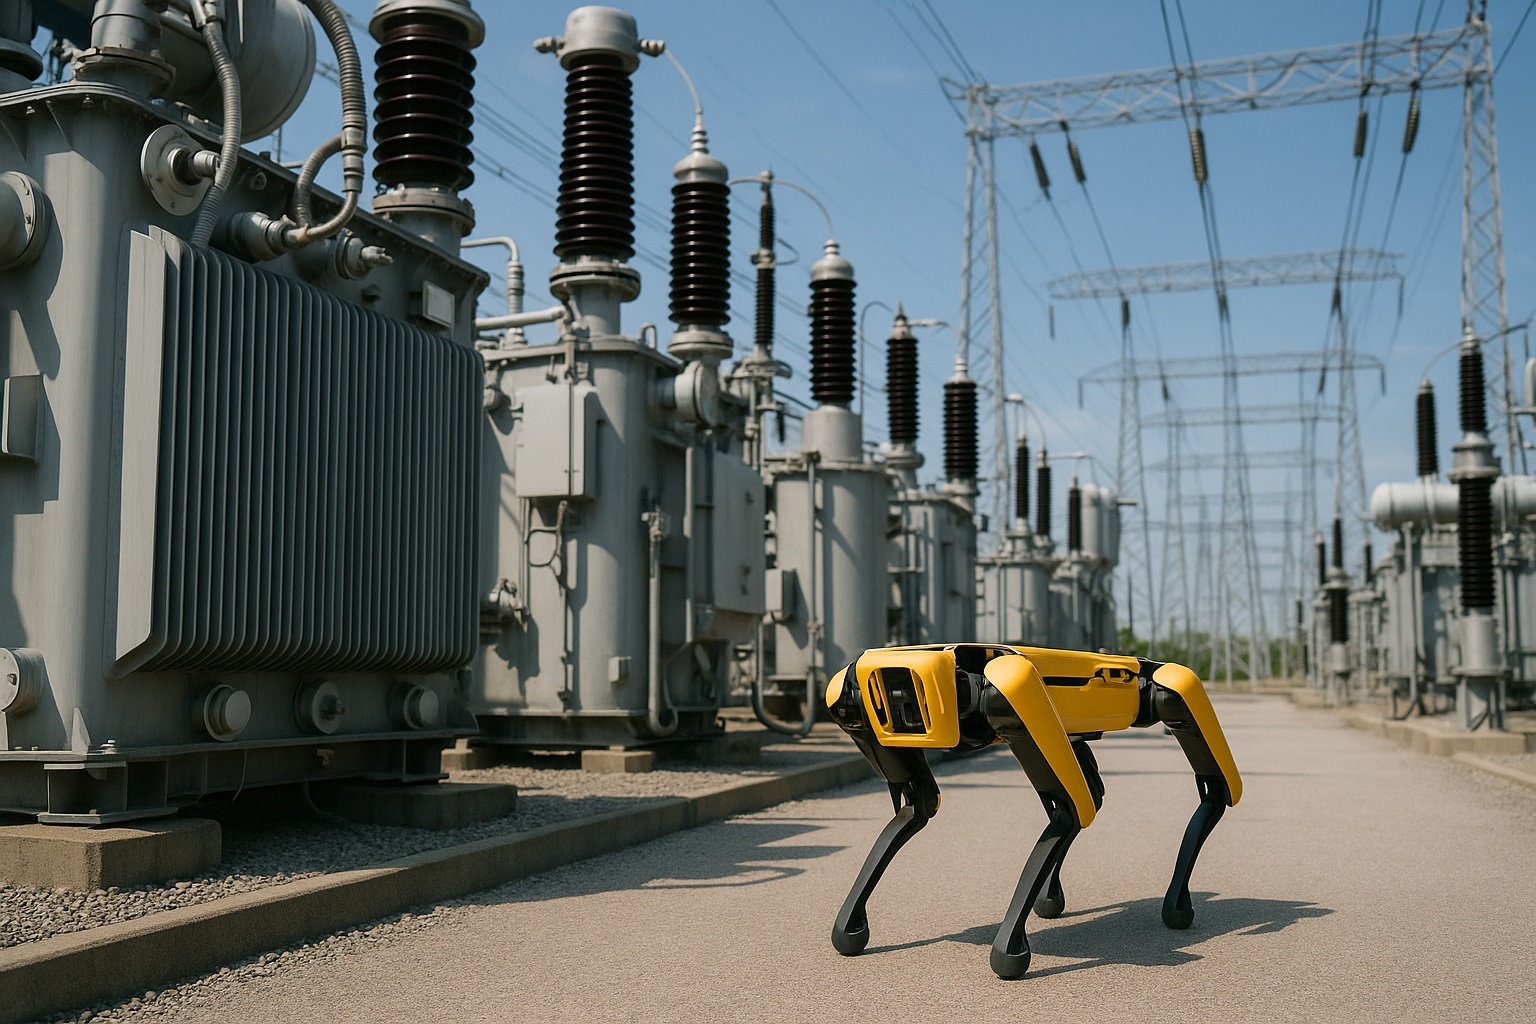
\includegraphics[width=0.8\textwidth]{figuras/fig_contextualizacao.jpg}
    \caption{Robô quadrúpede realizando inspeção em subestação de energia elétrica.}
    \legend{Fonte: O próprio autor.}
    \label{fig:contextualizacao}
\end{figure}

Nas últimas décadas, a robótica móvel autônoma emergiu como uma solução promissora para automatizar tarefas de inspeção em diversos setores industriais \cite{Wei2024Advancements}. A aplicação de robôs em subestações elétricas oferece o potencial de aumentar a frequência e a consistência das inspeções, reduzir custos operacionais, minimizar a exposição humana a riscos e coletar dados de forma mais sistemática e detalhada \cite{RobotnikSubstationBenefits}. Equipados com uma variedade de sensores, como câmeras visuais e térmicas, \ac{LiDAR}, microfones e detectores de gás, os robôs podem monitorar equipamentos, detectar anomalias como superaquecimento, descargas parciais, vazamentos ou danos estruturais e navegar autonomamente pelo ambiente complexo da subestação.
O desenvolvimento de sistemas de navegação autônoma para esses robôs é um campo de pesquisa ativo. Abordagens baseadas em \ac{SLAM} permitem que os robôs construam mapas do ambiente e se localizem dentro deles simultaneamente \cite{Kim2018SLAMMapping}. Modelos tridimensionais pré-existentes, muitas vezes gerados por técnicas como fotogrametria ou escaneamento a laser – áreas de expertise do grupo de pesquisa onde este trabalho se insere –, também podem ser utilizados para auxiliar na navegação e no planejamento de rotas. Além disso, a integração com tecnologias como \ac{RV} e \ac{RA} abre novas possibilidades para a operação remota e a visualização de dados coletados pelos robôs \cite{Ding2022QuadrupedDigitalTwin}.
Contudo, apesar dos avanços significativos, muitas das soluções atuais de inspeção robótica em subestações ainda operam predominantemente com base em rotas pré-definidas ou otimizadas para cobertura de área \cite{TJH2b2023Trends}. Essa abordagem, embora útil para tarefas de monitoramento rotineiro (ronda), pode não ser a mais eficiente ou eficaz para uma inspeção verdadeiramente investigativa. Eventos anômalos ou condições que exigem atenção imediata podem ocorrer fora da rota planejada ou exigir uma resposta dinâmica que vai além do simples seguimento de um caminho. A capacidade de um robô não apenas seguir uma rota, mas perceber ativamente seu entorno, interpretar múltiplos estímulos sensoriais de forma integrada e reagir inteligentemente a eventos inesperados, direcionando sua atenção para onde ela é mais necessária, representa um desafio e uma oportunidade significativa para a próxima geração de sistemas de inspeção autônoma.

Apesar do potencial da robótica autônoma, a implementação eficaz de sistemas de inspeção em subestações elétricas enfrenta desafios significativos que limitam o desempenho e a confiabilidade das abordagens atuais, majoritariamente baseadas em rotas pré-definidas \cite{TJH2b2023Trends}. A simples execução de rondas programadas, embora útil para cobertura sistemática, falha em abordar a necessidade de uma inspeção dinâmica e focada em eventos anômalos que podem surgir inesperadamente no ambiente complexo e muitas vezes hostil de uma subestação \cite{Wei2024Advancements}. A verdadeira inteligência em inspeção reside na capacidade do robô de perceber, interpretar e reagir adequadamente a estímulos ambientais em tempo real, adaptando sua trajetória e foco de inspeção conforme necessário.
A navegação autônoma robusta neste ambiente é particularmente desafiadora devido a uma confluência de fatores ambientais e operacionais. Primeiramente, a presença de altos níveis de interferência eletromagnética ou \ac{EMI}, inerente às operações de alta tensão, pode afetar severamente o funcionamento de sensores eletrônicos e sistemas de comunicação do robô, comprometendo a aquisição de dados e a própria capacidade de navegação \cite{He2007EMCSubstation,tdworld2024Challenges}. Sensores de localização como GPS podem ser indisponíveis ou imprecisos, a ponto de os sistemas de navegação relatados para inspeção de subestação recorrerem à combinação de DGPS com odometria \cite{Yan2024CombinedNav}, e até mesmo sensores como \ac{LiDAR} e câmeras podem sofrer interferências ou degradação de desempenho.
Adicionalmente, o ambiente físico das subestações impõe obstáculos consideráveis. A abundância de estruturas metálicas (equipamentos, grades, postes) pode causar múltiplas reflexões e oclusões para sensores baseados em ondas, como \ac{LiDAR} e radar, além de dificultar a interpretação de dados visuais \cite{Wijayathunga2023Challenges, Cai2025AttentionSeg}. A variabilidade extrema nas condições de iluminação, alternando entre luz solar direta, sombras profundas e iluminação artificial noturna, representa um desafio significativo para algoritmos de visão computacional. A necessidade de operar tanto em ambientes internos quanto externos adiciona outra camada de complexidade, exigindo que o sistema de navegação se adapte a diferentes tipos de terreno, condições atmosféricas e características espaciais \cite{Alatise2020Review}. A presença de obstáculos fixos e potencialmente dinâmicos (veículos de manutenção, pessoal) também requer capacidades avançadas de detecção e desvio.
Portanto, o problema central de pesquisa abordado nesta tese reside na \textbf{limitação dos atuais \textit{frameworks} de navegação robótica para inspeção de subestações em lidar de forma adaptativa e reativa com a complexidade ambiental e a natureza dinâmica dos eventos de interesse}. Falta uma abordagem que use a saliência do que é percebido para guiar ativamente a navegação, permitindo que o robô seja ``atraído'' por anomalias relevantes e ``repelido'' por perigos, e que o faça de modo a permitir atribuir qual mecanismo entrega qual efeito. É esse recorte --- a \emph{lógica de decisão} que arbitra entre inspecionar e se afastar, e não a cadeia de percepção que a alimenta --- que esta tese ataca. A \autoref{fig:problema_pesquisa} mostra um infográfico com uma representação do problema da pesquisa.

\section{Problema de Pesquisa}
\label{sec:intro-problema}

%% Secao preenchida em 13/11/2026. Ela existia apenas com titulo e figura, de modo
%% que a pergunta de pesquisa nao estava enunciada em lugar algum do documento. As
%% subperguntas abaixo sao, uma a uma, o contraste experimental que as responde.

Robôs de inspeção de subestações em operação seguem rondas pré-programadas: o percurso
é fixo e não se altera em função do que o robô percebe no caminho
\cite{TJH2b2023Trends,Liu2016VisualNavSubstation}. A literatura que propõe superar essa
limitação acopla percepção e reação em sistemas que percebem, decidem e se desviam ao
mesmo tempo, e relata o desempenho \emph{agregado} do conjunto. Daí decorre o problema
desta tese, que é de atribuição e não de desempenho: quando uma arquitetura desse tipo
inspeciona mais e se afasta mais de um risco do que uma ronda fixa, não se sabe
\emph{qual} de seus mecanismos produziu cada efeito --- e a comparação contra a ronda
fixa não ajuda a descobrir, porque a ronda fixa não dispõe de mecanismo algum para
deixar a rota e perde por construção.

Essa indeterminação tem consequência prática. Quem for implantar um supervisor de
inspeção precisa decidir onde investir: em perceber melhor para ponderar alvos, em
expressar o risco no planejamento deliberativo, em dar memória temporal ao sinal de
perigo, ou em nenhuma dessas coisas. Sem atribuição, a decisão é tomada por analogia
com um resultado agregado que pode ter vindo de outro componente. E há um custo que o
relato agregado esconde: uma precedência de segurança que funciona bem também recusa
inspeções legítimas, e esse preço raramente é medido.

Formula-se, assim, a pergunta central:

\begin{quote}
Em uma arquitetura de inspeção que acopla o que o robô percebe à forma como ele reage,
\emph{qual mecanismo responde por qual efeito, e a que custo} --- quando cada mecanismo
é trocado ou removido isoladamente, mantidos o mesmo controlador de navegação, o mesmo
cenário e o mesmo protocolo de medida?
\end{quote}

Ela se desdobra em seis subperguntas, cada uma amarrada a um contraste executado:

\begin{enumerate}
    \item \textbf{Origem do afastamento.} Diante de um risco \emph{estático} sobre a
    rota de patrulha, o afastamento observado é produzido pela ponderação reativa ou
    pela expressão deliberativa da repulsão no \textit{costmap}? \emph{Contraste:}
    patrulha fixa com a mesma zona de exclusão e sem supervisor reativo, contra a
    ablação que retém a inspeção reativa, contra a ablação sem zona de exclusão
    (Seção~\ref{sec:res-ablacao}).

    \item \textbf{Critério de seleção.} Ponderar o alvo por saliência produz desfecho
    diferente de simplesmente escolher o mais próximo? \emph{Contraste:} variante que
    difere \emph{apenas} na regra de seleção, nos três cenários
    (Seção~\ref{sec:res-heu}).

    \item \textbf{Modo de disparo e persistência.} Substituir o campo com limiar e
    decaimento por detecção bruta altera o desfecho de segurança quando um risco está
    colocalizado com uma anomalia mais saliente? \emph{Contraste:} heurística genérica
    de detectar--selecionar--desviar--retornar sobre o \emph{mesmo} controlador
    Nav2/MPPI (Seção~\ref{sec:res-heu}), com a ressalva de que disparo e persistência
    variam em conjunto (Seção~\ref{sec:res-ameacas}).

    \item \textbf{Custo da precedência.} Qual é o preço, em inspeções perdidas e em
    tempo de missão, de conceder prioridade categórica ao canal de risco? \emph{
    Contraste:} cenário com risco marginalmente elegível
    (Seção~\ref{sec:res-custo-precedencia}) e varreduras de limiar e de histerese
    (Seções~\ref{sec:res-sens-limiar} e~\ref{sec:res-histerese}).

    \item \textbf{Papel do aprendizado.} Uma tabela de valor treinada com recompensa
    aumentada pelo campo, \emph{selecionando} as ações, supera a regra fixa de
    precedência? \emph{Contraste:} linha de base \textsc{Q-driven} nos três cenários
    (Seção~\ref{sec:res-qdriven}).

    \item \textbf{Métrica contra propriedade física.} Quanto da completude de inspeção
    relatada é propriedade do comportamento e quanto é do critério de confirmação
    adotado? \emph{Contraste:} varredura de ruído de percepção e reavaliação
    retrospectiva do limiar de confirmação sobre os mesmos registros
    (Seções~\ref{sec:res-ruido} e~\ref{sec:res-inspecao}).
\end{enumerate}

A resposta a essas subperguntas --- inclusive quando ela é negativa, como nos itens 2
e~5 --- é o que esta tese oferece como contribuição, e não a demonstração de que um
robô de inspeção pode desviar de um obstáculo.

\begin{figure}[h]
    \centering
    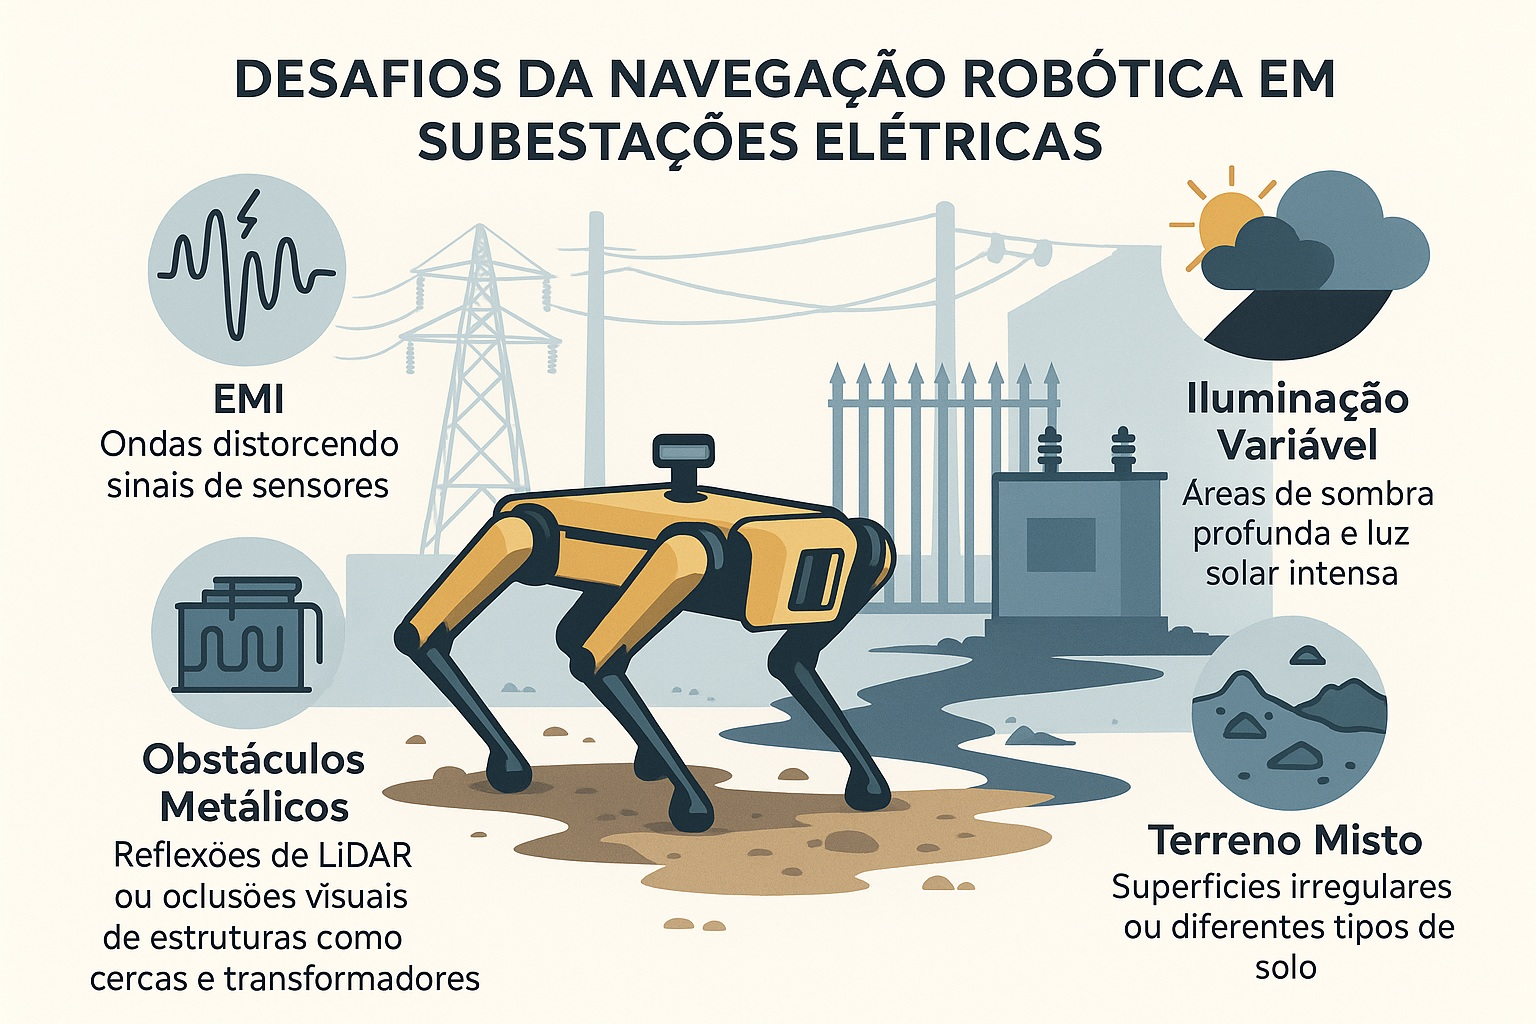
\includegraphics[width=0.8\textwidth]{figuras/fig_problema_pesquisa.jpg}
    \caption{Desafios da Navegação Robótica em Subestações Elétricas.}
    \legend{Fonte: O próprio autor.}
    \label{fig:problema_pesquisa}
\end{figure}


\section{Justificativa e Relevância}

A presente pesquisa se justifica pela necessidade premente de aprimorar os métodos de inspeção em subestações elétricas, superando as limitações das abordagens manuais e das atuais soluções robóticas baseadas em rotas. A relevância deste trabalho reside tanto em suas potenciais contribuições práticas para o setor elétrico quanto em seus avanços científicos no campo da robótica autônoma.
Do ponto de vista prático, o desenvolvimento de uma arquitetura de navegação capaz de adaptar a ronda de inspeção ao que o robô percebe tem o potencial de impactar significativamente a operação e manutenção de subestações. Ao permitir inspeções mais frequentes, consistentes e detalhadas, a solução proposta pode levar a uma detecção mais precoce de falhas e anomalias, contribuindo para a redução de custos com manutenção corretiva e minimizando o risco de interrupções no fornecimento de energia \cite{Wei2024Advancements}. A automação de tarefas de inspeção, especialmente em ambientes perigosos ou de difícil acesso, aumenta a segurança dos trabalhadores, reduzindo sua exposição a riscos elétricos e ambientais \cite{Anybotics2023Advantages}. Além disso, a capacidade de reação inteligente a eventos inesperados pode otimizar o tempo de inspeção, focando os recursos do robô nas áreas que realmente demandam atenção, aumentando a eficiência geral do processo \cite{EnergyRobotics2024Future}.
%% Reescrito em 12/11/2026. O texto anterior reivindicava fusão sensorial
%% heterogênea e aprendizado por reforço como as contribuições científicas do
%% trabalho -- promessa da proposta de qualificação que a avaliação não sustenta,
%% conforme a Seção~\ref{sec:intro-escopo}. As referências foram preservadas: elas
%% agora situam as frentes da literatura, em vez de atestar entregas desta tese.
Cientificamente, esta tese ataca uma lacuna de \emph{atribuição}. A literatura recente de navegação para inspeção avança em duas frentes --- a fusão de sensores heterogêneos, incluindo \ac{LiDAR}, visão computacional, visão térmica, áudio e ultrassom, para construir percepção situacional robusta sob oclusão e degradação sensorial \cite{Alatise2020Review, Ou2024SensorFusionDRL}, em instalação cujo rigor eletromagnético é requisito de projeto reconhecido \cite{He2007EMCSubstation}, e as políticas aprendidas para decidir como reagir ao que se percebe \cite{Zhu2017, Kahn2021} ---, e ambas relatam ganhos agregados de desempenho. O que raramente se estabelece é \emph{qual mecanismo} produz cada ganho. Um sistema que percebe, decide e desvia melhora a inspeção por várias razões simultâneas, e a comparação contra uma ronda fixa é vencida por construção, já que a ronda fixa não dispõe de mecanismo para deixar a rota. Esta tese adota a posição oposta: formula o acoplamento entre o que se percebe e como se reage como um campo escalar de atração e repulsão com precedência categórica de segurança, afastando-se tanto do planejamento de caminho puro quanto do controlador puramente reativo \cite{Wijayathunga2023Challenges}, e em seguida desmonta experimentalmente a própria proposta --- comparando-a contra uma heurística genérica executada sobre o mesmo controlador, trocando um fator de cada vez e ablacionando a resposta de segurança em seus componentes --- para declarar o que a evidência sustenta e o que não sustenta. A contribuição é esse conjunto de atribuições, inclusive as negativas, sobre uma classe de arquitetura que vem sendo adotada sem tal escrutínio. Finalmente, ao tratar dos desafios específicos das subestações elétricas, o trabalho contribui com conhecimento aplicável a outros domínios que exigem navegação robótica robusta em condições adversas.
Portanto, a pesquisa proposta é relevante por oferecer uma solução tecnológica com potencial de impacto direto na indústria de energia elétrica, ao mesmo tempo que avança o conhecimento científico em áreas chave da robótica autônoma, como a arbitragem entre comportamentos, a navegação adaptativa e a avaliação experimental de sistemas robóticos. A \autoref{fig:justificativa} ilustra a relevância da pesquisa.

\begin{figure}[h]
    \centering
    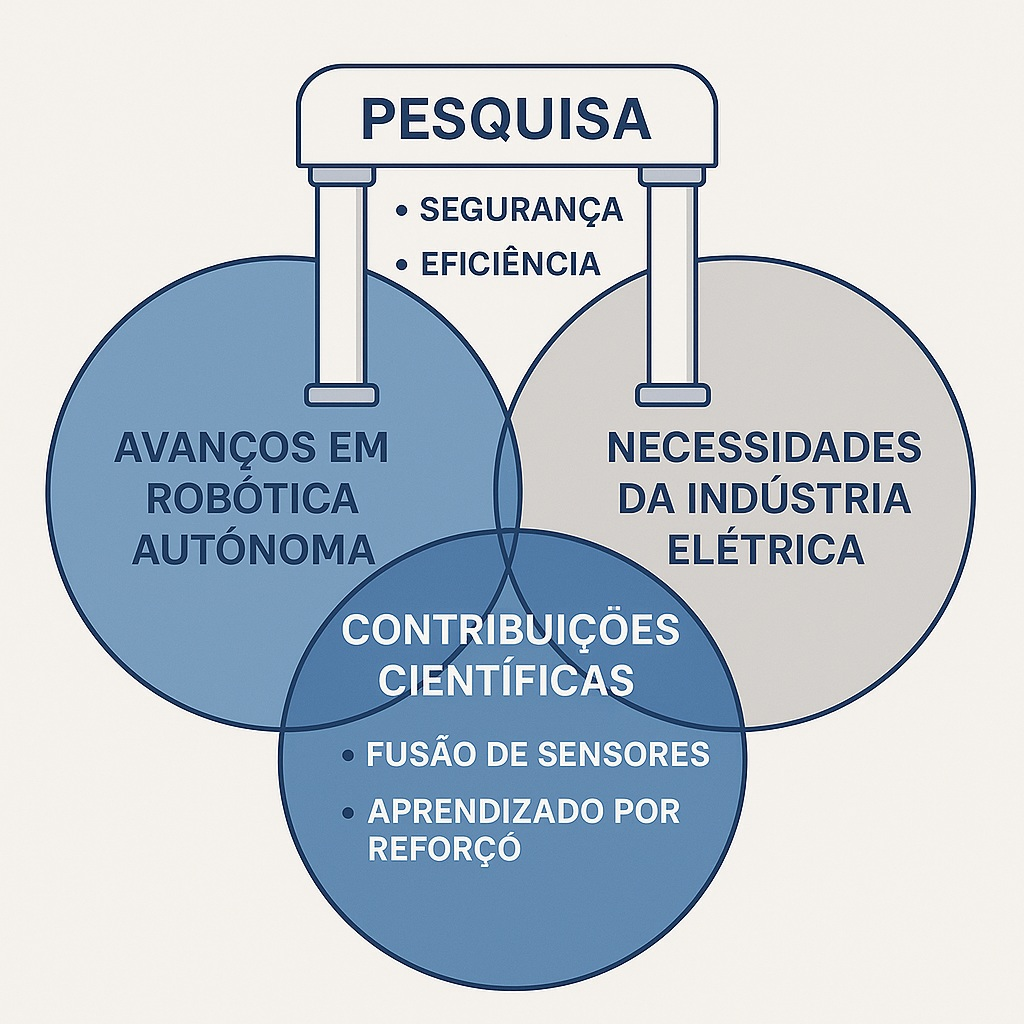
\includegraphics[width=0.8\textwidth]{figuras/fig_justificativa.jpg}
    \caption{Relevância da Pesquisa: Interseção entre Robótica Autônoma e Necessidades da Indústria Elétrica.}
    \legend{Fonte: O próprio autor.}
    \label{fig:justificativa}
\end{figure}


\section{Objetivos}

\subsection{Objetivo Geral}

Projetar, implementar e avaliar uma arquitetura de navegação deliberativo-reativa de
duas camadas para inspeção de subestações elétricas, na qual uma patrulha
deliberativa de sensoriamento ativo conduz os sensores pelo sítio e uma camada
reativa converte a saliência sensorial em um campo de atração/repulsão que aciona,
por limiar, a aproximação de anomalias e o afastamento de riscos --- atribuindo
experimentalmente a cada mecanismo o efeito que ele de fato produz.

\subsection{Objetivos Específicos}

\begin{enumerate}
    \item \textbf{Formular o campo de atração--repulsão.} Definir um campo escalar
    com memória, construído a partir de modalidade, intensidade e distância dos
    eventos percebidos, e uma regra de arbitragem que imponha segurança antes de
    inspeção como precedência categórica, e não como disputa de magnitude.

    \item \textbf{Projetar a camada reativa.} Especificar uma máquina de estados
    finitos que preempte a patrulha diante de eventos salientes, emita metas focadas
    de aproximação ou recuo a uma pilha de navegação madura e devolva o controle à
    patrulha, mantendo separadas as etapas de controle e de crédito de inspeção.

    \item \textbf{Integrar repulsão deliberativa e reativa.} Combinar o recuo
    reativo a uma zona de exclusão persistente projetada no \textit{costmap} global,
    de modo a tratar riscos que bloqueiam a própria rota de patrulha.

    \item \textbf{Avaliar com linhas de base que isolem o mecanismo.} Comparar a
    arquitetura contra uma patrulha fixa, contra um controlador de campo potencial
    artificial e --- sobretudo --- contra uma heurística genérica de
    detectar--selecionar--desviar--retornar sobre o \emph{mesmo} controlador, de
    modo a separar o campo do mero ato de desviar.

    \item \textbf{Atribuir efeitos a mecanismos por ablação.} Desmontar a resposta
    de segurança em seus componentes --- zona de exclusão, recuo reativo, ponderação
    por saliência, modo de disparo --- e medir a contribuição de cada um, declarando
    explicitamente o que a evidência sustenta e o que não sustenta.

    \item \textbf{Quantificar os custos da precedência.} Medir o preço, em inspeções
    perdidas e em tempo de missão, da prioridade rígida concedida ao canal de risco,
    em vez de tratá-lo como efeito colateral aceitável não examinado.

    \item \textbf{Entregar um pacote reprodutível.} Publicar código, mundo simulado,
    dados por execução e \textit{scripts} de análise, de modo que todo denominador
    relatado possa ser conferido.
\end{enumerate}

%% Secao criada em 13/11/2026. As contribuicoes estavam dispersas entre objetivos,
%% metodologia e conclusao, o que deixava o leitor sem saber o que e herdado, o que e
%% modificacao e qual evidencia sustenta cada uma. Cada item declara os cinco campos
%% na mesma ordem, e nenhum deles omite a limitacao.
\section{Contribuições}
\label{sec:intro-contribuicoes}

Cada contribuição é declarada em cinco campos --- componente herdado, modificação
proposta, evidência produzida, conhecimento novo e limitação ---, de modo que o que é
reivindicado como original possa ser separado do que é reaproveitado e confrontado com
a evidência correspondente. Duas das seis contribuições são \emph{resultados
negativos}: eles são declarados como contribuição porque delimitam uma classe de
arquitetura que vem sendo adotada sem esse escrutínio, e não porque confirmam a
proposta.

\begin{enumerate}
    \item \textbf{Campo de atração--repulsão com canais de memória e precedência
    categórica.} \emph{Herdado:} campos de atração e repulsão para navegação
    \cite{Arkin1989,Barraquand1992} e prioridade fixa entre camadas de comportamento
    \cite{Brooks1986}. \emph{Modificação:} o canal de risco não disputa magnitude com
    o canal de inspeção --- ele governa por precedência categórica sempre que um risco
    é elegível --- e carrega memória própria, com limiar de elegibilidade e decaimento
    (Seção~\ref{sec:prop-campo}). \emph{Evidência:} contraste contra uma heurística
    genérica de detectar--selecionar--desviar--retornar executada sobre o mesmo
    controlador Nav2/MPPI, e varreduras de limiar e de histerese
    (Seções~\ref{sec:res-heu}, \ref{sec:res-sens-limiar} e~\ref{sec:res-histerese}).
    \emph{Conhecimento novo:} nos cenários executados, o que separa esta camada de uma
    heurística de desviar e retornar é a persistência temporal do canal de risco; a
    ponderação por saliência não produziu diferença detectável no mesmo conjunto de
    condições. \emph{Limitação:} no contraste executado, o modo de disparo e a
    persistência variam em conjunto, de modo que não são fatores separáveis com as
    configurações rodadas (Seção~\ref{sec:res-ameacas}).

    \item \textbf{Expressão deliberativa da repulsão acoplada ao recuo reativo.}
    \emph{Herdado:} inflação de obstáculos em mapa de custos na pilha de navegação
    \cite{Macenski2022}. \emph{Modificação:} projeção persistente do risco detectado
    como zona de exclusão no mapa de custos global, acoplada à preempção reativa, para
    tratar riscos que bloqueiam a própria rota de patrulha
    (Seção~\ref{sec:prop-keepout}). \emph{Evidência:} ablação em três braços --- com
    zona e sem supervisor, com ambos, e sem zona (Seção~\ref{sec:res-ablacao}).
    \emph{Conhecimento novo:} sobre um risco estático na rota, o afastamento é
    atribuível à zona de exclusão deliberativa e não à ponderação reativa; e sem ela o
    recuo reativo sozinho não resolveu o risco dentro do orçamento de execução concedido
    --- nenhuma execução concluiu a missão. \emph{Limitação:} o resultado vale para o
    cenário de risco estático sobre a rota e para as configurações estudadas; ausência
    de benefício adicional detectado não demonstra equivalência geral de componentes.

    \item \textbf{Desenho de avaliação que isola o mecanismo.} \emph{Herdado:}
    protocolos de comparação por simulação em navegação autônoma. \emph{Modificação:} a
    heurística comparada roda sobre o \emph{mesmo} controlador Nav2/MPPI e a mesma
    camada de eventos, o que remove o controlador como confundidor, e cada variante
    troca um fator por vez (Capítulo~\ref{cap:avaliacao}). \emph{Evidência:} $32$ pares
    configuração--cenário, $320$ execuções tentadas e $311$ válidas, com família de
    comparação primária de $15$ testes declarada a priori quanto à regra de
    multiplicidade (Seções~\ref{sec:setup-censo} e~\ref{sec:res-familias}).
    \emph{Conhecimento novo:} o ganho sobre uma ronda fixa não é informativo sobre
    mecanismo; o contraste informativo é contra a mesma arquitetura com um fator
    trocado. \emph{Limitação:} um único \textit{layout} e uma única distribuição de
    eventos por cenário --- o que as repetições estabelecem é repetibilidade naquelas
    condições, não validade externa.

    \item \textbf{Custo medido da precedência de segurança.} \emph{Herdado:} a prática
    de dar prioridade à segurança, corrente desde as arquiteturas em camadas.
    \emph{Modificação:} um cenário desenhado para tornar esse custo \emph{observável},
    com um risco marginalmente elegível cuja presença não justifica o recuo
    (Seção~\ref{sec:res-custo-precedencia}). \emph{Evidência:} supressão da atração por
    cerca de $70$~s e renúncia a uma de quatro inspeções em $10/10$ execuções.
    \emph{Conhecimento novo:} a precedência categórica tem preço quantificável e
    reprodutível, em inspeções perdidas e em tempo de missão, em vez de efeito
    colateral aceitável não examinado. \emph{Limitação:} o valor depende do limiar de
    elegibilidade e da geometria do cenário, e não é uma constante da arquitetura.

    \item \textbf{Resultado negativo: o critério de seleção não teve efeito
    detectável.} \emph{Herdado:} a ponderação de alvos por saliência.
    \emph{Modificação:} variante que difere \emph{apenas} na regra de seleção ---
    o alvo mais próximo em lugar do mais saliente (Seção~\ref{sec:res-heu}).
    \emph{Evidência:} desfechos discretos idênticos ao longo das dez execuções nos
    cenários de referência e distribuições sobrepostas no cenário adverso, com
    equivalência declarada por \ac{TOST} onde as margens a sustentam
    (Seção~\ref{sec:res-equivalencia}). \emph{Conhecimento novo:} nestes cenários, a
    saliência não domina a proximidade, o que redireciona o esforço de projeto para a
    arbitragem e sua extensão temporal. \emph{Limitação:} não detectar diferença não é
    equivalência, exceto onde o \ac{TOST} a declara com margem justificada; e a
    utilidade da saliência em outras distribuições de eventos não é eliminada.

    \item \textbf{Resultado negativo: a tabela de valor não substitui a regra de
    precedência.} \emph{Herdado:} \textit{Q-learning} tabular com recompensa aumentada.
    \emph{Modificação:} além da atualização passiva do método principal
    (Seção~\ref{sec:prop-atualizacao}), uma linha de base em que a tabela de valor
    \emph{seleciona} a ação executada, medida nos três cenários
    (Seção~\ref{sec:res-qdriven}). \emph{Evidência:} bloco de doze testes com correção
    interna de multiplicidade. \emph{Conhecimento novo:} a tabela de valor treinada com
    recompensa aumentada pelo campo não superou a regra fixa de precedência nas
    implementações comparadas. \emph{Limitação:} a comparação é entre as duas
    implementações efetivamente testadas --- a política atua em velocidade e foi
    treinada em simulador cinemático, enquanto o método envia metas ao Nav2/MPPI ---, e
    não entre os paradigmas de decisão em geral.
\end{enumerate}

Um sétimo item é artefato, e não conhecimento: o pacote reprodutível
--- código, mundo simulado, manifesto por execução e \textit{scripts} que regeneram as
tabelas de resultado a partir dos registros ---, cuja limitação está declarada no
Capítulo~\ref{cap:resultados}: as baterias já executadas não gravaram o identificador
de \textit{commit} por execução, o que não é recuperável retroativamente.

%% Secao criada em 12/11/2026. Registra, de frente e na introducao, o estreitamento
%% de escopo em relacao a proposta qualificada em 12/09/2026. O enquadramento e
%% deliberado: a decisao e do autor e a justificativa e a evidencia das proprias
%% simulacoes. A Secao~\ref{sec:conc-escopo} faz a retrospectiva e remete a esta.
\section{Delimitação de Escopo}
\label{sec:intro-escopo}

A proposta qualificada previa um \textit{framework} de cinco módulos --- aquisição
multissensorial, fusão sensorial heterogênea, detecção de eventos, decisão por
aprendizado por reforço e controle reativo integrado a \ac{SLAM} e a modelos
tridimensionais ---, no qual a decisão de aproximar-se de uma anomalia ou afastar-se
de um risco seria \emph{aprendida}. O que esta tese entrega é mais estreito e mais
fundo: a arquitetura de duas camadas do Capítulo~\ref{cap:proposta}, submetida a um
desenho experimental que atribui a cada mecanismo o efeito que ele de fato produz. O
estreitamento foi decidido ao longo do desenvolvimento, e decidido pelos resultados.
Cabe dizer quais resultados, e com que consequências.

\begin{enumerate}
    \item \textbf{O ganho de segurança não vem da ponderação reativa.} Uma patrulha
    fixa portando a mesma zona de exclusão disparada por detecção, e sem qualquer
    supervisor reativo, alcançou afastamento mínimo mediano de $1{,}73$~m, contra
    $1{,}71$~m da ablação que retém a inspeção reativa --- sem diferença
    estatisticamente detectável ($p_{\mathrm{Holm}}=0{,}4194$). O que a camada
    reativa acrescenta sobre a patrulha fixa são as inspeções ($3$ contra $0$ de
    $3$), não o afastamento. Um \textit{framework} organizado em torno da modulação
    do sinal de resposta estaria, portanto, organizado em torno do componente errado.

    \item \textbf{A tabela de valor não seleciona as ações executadas.} As transições
    da máquina de estados leem o campo bruto $\Phi$, e não o peso afetivo $\eta$ da
    atualização de valor; o movimento provém das metas enviadas ao Nav2/MPPI. Em
    consequência, uma varredura sobre $\eta$ não mede sensibilidade comportamental,
    e nenhum experimento conduzido atribuiu efeito observável à atualização. Treinar
    uma política sobre essa tabela exigiria política de exploração, mapeamento de
    ação para velocidade e comparação contra \textit{Q-learning} tabular comum ---
    um estudo próprio, e não um módulo a mais. Esse estudo foi posteriormente
    conduzido em sua forma executada e é relatado na Seção~\ref{sec:res-qdriven}:
    uma política tabular aprendida, selecionando a ação executada, não altera a
    completude de inspeção nem a segurança, e custa tempo na subtarefa reativa.

    \item \textbf{Percepção e localização realistas impediriam a atribuição.} Com uma
    cadeia de percepção real e localização estimada em tempo de execução, o erro de
    detecção e o erro de localização dominam a variância dos desfechos medidos.
    Diferenças de meio metro em afastamento mínimo, ou de dezenas de segundos em
    atraso de inspeção, deixam de ser atribuíveis à regra de arbitragem --- que é
    precisamente o objeto desta tese.
\end{enumerate}

Diante disso, três decisões de projeto foram tomadas, e são declaradas aqui como
\emph{controles de confundimento}, não como omissões. A saída da cadeia de percepção
foi abstraída em eventos --- modalidade, intensidade e posição ---, conforme a
Seção~\ref{sec:prop-sensoriamento}. A transformada de localização foi mantida fixa.
E a atualização de valor foi registrada como nota de projeto na
Seção~\ref{sec:prop-atualizacao}, com a ressalva explícita de que não governa o
comportamento avaliado. O preço dessas três escolhas é a validade externa: os
resultados falam da lógica de decisão da arquitetura, e não de um sistema pronto para
implantação, como a Seção~\ref{sec:prop-nao-abordado} delimita. O que elas compram é
a validade interna que torna a atribuição possível.

O objeto da tese, portanto, deslocou-se de \emph{integrar} para \emph{atribuir}. Essa
troca não reduziu a exigência experimental; aumentou-a. Onde a proposta previa
comparação contra métodos de rotas pré-definidas, a avaliação do
Capítulo~\ref{cap:avaliacao} acrescenta um controlador de campo potencial artificial,
uma heurística genérica de detectar--selecionar--desviar--retornar executada sobre o
\emph{mesmo} controlador Nav2/MPPI, variantes de um único fator e ablações da
resposta de segurança, com tamanhos de efeito, intervalos de confiança, testes
livres de distribuição e de equivalência, correção de Holm e denominadores
explícitos.

Nada do que a proposta reuniu foi descartado do documento. A fundamentação sobre
fusão sensorial heterogênea e aprendizado por reforço permanece nos
Capítulos~\ref{cap:fundamentacao} e~\ref{cap:revisao}, porque é o contexto que
motivou a investigação e que situa a arquitetura entre as alternativas. A
heterogeneidade sensorial permanece no modelo de eventos, que distingue as
modalidades térmica, acústica e de risco com parâmetros próprios. A formulação de
valor permanece como nota de projeto, com o resíduo completo reportado no
Capítulo~\ref{cap:resultados}. O que mudou foi o que se \emph{reivindica} como
entregue e demonstrado. A Tabela~\ref{tab:intro-escopo} faz essa correspondência,
objetivo por objetivo.

\begin{table}[htb]
\centering
\caption{Correspondência entre os objetivos específicos da proposta de qualificação e
o que esta tese entrega.}
\label{tab:intro-escopo}
\footnotesize
\begin{tabular}{p{0.30\textwidth}p{0.17\textwidth}p{0.42\textwidth}}
\hline
\textbf{Objetivo da proposta} & \textbf{Situação} & \textbf{Onde está nesta tese}\\
\hline
Propor arquitetura modular (fusão, detecção, decisão aprendida, controle integrado a
\ac{SLAM} e modelos 3D) &
Entregue em forma modificada &
Arquitetura de duas camadas do Capítulo~\ref{cap:proposta}, com abstração de eventos
no lugar do módulo de fusão e acionamento por limiar no lugar da decisão aprendida\\
\hline
Investigar e implementar técnicas de fusão sensorial &
Não entregue &
Tratada como fundamentação (Capítulos~\ref{cap:fundamentacao}
e~\ref{cap:revisao}); substituída pela abstração de eventos
(Seção~\ref{sec:prop-sensoriamento}) e nomeada em trabalhos futuros
(Seção~\ref{sec:conc-futuro})\\
\hline
Desenvolver e treinar modelo de aprendizado por reforço &
Entregue como formulação, análise e comparação executada &
Seção~\ref{sec:prop-atualizacao}; resíduo completo
$|\alpha\delta+\eta\Phi|$ no Capítulo~\ref{cap:resultados}; e baseline
\textsc{Q-driven} --- tabela $Q$ treinada com recompensa aumentada por $\Phi$,
selecionando a ação executada --- medido contra o método nos três cenários
(Seção~\ref{sec:res-qdriven})\\
\hline
Integrar com \ac{SLAM} e modelos tridimensionais &
Não entregue como proposto &
Transformada de localização mantida fixa, por controle de confundimento
(Seção~\ref{sec:prop-nao-abordado})\\
\hline
Validar por simulação contra métodos de rotas pré-definidas &
Entregue e ampliado &
Capítulo~\ref{cap:avaliacao}: além da patrulha fixa, campo potencial artificial,
heurística genérica sobre o mesmo controlador, variantes de um fator e ablações,
com tratamento estatístico completo\\
\hline
\end{tabular}
\end{table}

\section{Metodologia}

A abordagem adotada foi construtiva e experimental. A pesquisa foi conduzida nas
seguintes fases:

\begin{enumerate}
    \item \textbf{Revisão da literatura.} Revisão crítica da
    literatura em robótica móvel autônoma, navegação em ambientes complexos, fusão
    de sensores heterogêneos, aprendizado por reforço aplicado à robótica e inspeção
    de subestações elétricas, consolidando o estado da arte e identificando as
    lacunas que o trabalho ataca (Capítulos~\ref{cap:fundamentacao}
    e~\ref{cap:revisao}).

    \item \textbf{Projeto da arquitetura.} Definição da separação em camada
    deliberativa e camada reativa, da formulação do campo com seus dois canais de
    memória, da regra de precedência e da máquina de estados, bem como da expressão
    deliberativa da repulsão (Capítulo~\ref{cap:proposta}).

    \item \textbf{Implementação.} Implementação como pacotes ROS~2 Humble, com
    navegação pela pilha Nav2 (planejador global NavfnPlanner e controlador MPPI) e
    simulação física em Gazebo Fortress. A saída da cadeia de percepção foi
    abstraída como eventos --- modalidade, intensidade e posição ---, simplificação
    deliberada e delimitada, discutida na Seção~\ref{sec:prop-nao-abordado}.

%% Corrigido em 13/11/2026: a contagem anterior ("vinte configuracoes") nao fechava
    %% com a matriz nem com os dados em disco. O censo da Tabela~\ref{tab:setup-censo} da
    %% 32 pares configuracao-cenario e 320 execucoes tentadas.
    \item \textbf{Avaliação experimental.} Execução de uma matriz de $32$ pares
    configuração--cenário sobre seis cenários, com dez execuções tentadas por par ---
    $320$ ao todo, das quais $311$ válidas ---, abrangendo linhas de base, ablações,
    cenários de conflito e de risco emergente, varreduras de limiar e de histerese e
    perturbações de ruído de percepção (Capítulo~\ref{cap:avaliacao}, com o censo na
    Seção~\ref{sec:setup-censo}).

    \item \textbf{Análise estatística.} Comparações por testes livres de
    distribuição, com tamanhos de efeito, intervalos \textit{bootstrap} e correção
    de multiplicidade dentro de uma família de comparação declarada, mantendo
    explícita a fronteira entre alegações primárias e exploratórias
    (Capítulo~\ref{cap:resultados}).
\end{enumerate}

A \autoref{fig:metodologia} apresenta um fluxograma da metodologia geral.

\begin{figure}[h]
    \centering
%% Figura refeita em 12/11/2026. A versao anterior (fig_metodologia.jpg, ainda em
%% figuras/ mas nao mais referenciada) trazia "PROJETO E DESENVOLVIMENTO DO
%% FRAMEWORK" e "IMPLEMENTACAO E TREINAMENTO DOS COMPONENTES CHAVE" -- vocabulario
%% da proposta de qualificacao. Nao houve treinamento, e as fases agora sao as
%% efetivamente executadas, na mesma ordem do texto desta secao.
    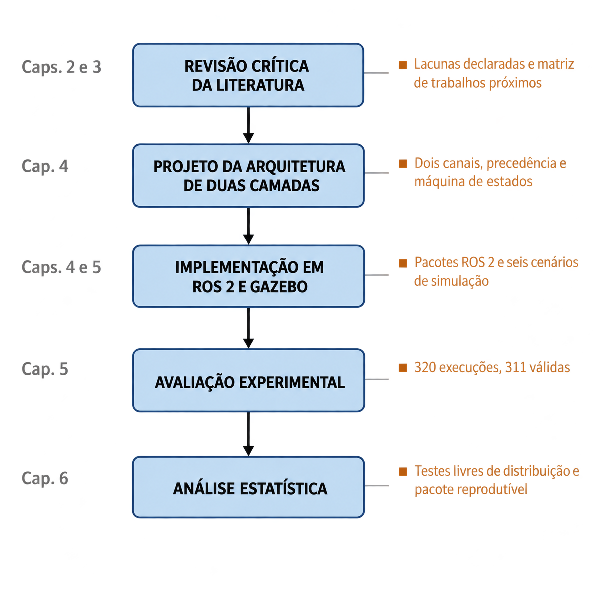
\includegraphics[width=0.8\textwidth]{figuras/fig_metodologia.pdf}
    \caption{Fluxograma da metodologia adotada.}
    \legend{Fonte: O próprio autor.}
    \label{fig:metodologia}
\end{figure}

\section{Organização do Documento}

\begin{itemize}
    \item \textbf{Capítulo~\ref{cap:introducao} --- Introdução.} Contextualiza a
    inspeção robótica em subestações, define o problema de pesquisa, justifica a
    relevância do trabalho, estabelece os objetivos, delimita o escopo em relação à
    proposta de qualificação (Seção~\ref{sec:intro-escopo}) e descreve a metodologia
    adotada.

    \item \textbf{Capítulo~\ref{cap:fundamentacao} --- Fundamentação Teórica.}
    Apresenta os fundamentos de fusão sensorial heterogênea, aprendizado por reforço,
    características operacionais de subestações elétricas, sistemas robóticos e
    ROS/ROS2, e navegação reativa em robótica móvel.

%% Renomeado em 13/11/2026 junto com o Capitulo~\ref{cap:revisao}: nao ha protocolo
    %% de revisao sistematica executado, e o capitulo agora declara seu criterio de
    %% selecao e o alcance dele.
    \item \textbf{Capítulo~\ref{cap:revisao} --- Revisão Crítica da Literatura.}
    Discute o estado da arte nas áreas relevantes, declara como os trabalhos foram
    selecionados e identifica as lacunas que esta pesquisa visa preencher.

    \item \textbf{Capítulo~\ref{cap:proposta} --- Arquitetura Proposta.} Detalha a
    arquitetura de duas camadas: o campo de atração--repulsão e seus canais com
    memória, a regra de precedência categórica, a máquina de estados
    \textsc{Stay Alert}, a zona de exclusão deliberativa e a abstração de eventos.

    \item \textbf{Capítulo~\ref{cap:avaliacao} --- Avaliação Experimental.} Descreve
    o ambiente de simulação, os cenários, a matriz experimental, as métricas, os
    hiperparâmetros e o pacote de reprodutibilidade.

    \item \textbf{Capítulo~\ref{cap:resultados} --- Resultados e Discussão.}
    Apresenta os resultados, atribui efeitos a mecanismos por ablação, quantifica os
    custos da precedência de segurança e enumera as ameaças à validade.

    \item \textbf{Capítulo~\ref{cap:conclusao} --- Conclusão.} Sintetiza as
    atribuições estabelecidas, delimita os limites da evidência, retoma a delimitação de escopo da
    Seção~\ref{sec:intro-escopo} e aponta direções para trabalhos futuros.
\end{itemize}


% ----------------------------------------------------------
% Fundamentação Teórica
% ----------------------------------------------------------
\chapter{Fundamentação Teórica}
\label{cap:fundamentacao}

Este capítulo apresenta os fundamentos teóricos que contextualizam a investigação.
São abordados cinco temas: fusão sensorial heterogênea, aprendizado por reforço,
inspeção em subestação de energia elétrica, sistemas robóticos e ROS/ROS2, e
navegação reativa em robótica móvel.

Convém explicitar, desde já, a relação entre esses fundamentos e o que foi
efetivamente construído. Os cinco temas delimitam o espaço de projeto no qual a
investigação se moveu e justificam as decisões tomadas; eles \emph{não} descrevem,
um a um, componentes do sistema avaliado. Em particular, a arquitetura apresentada
no Capítulo~\ref{cap:proposta} abstrai a cadeia de percepção em eventos, de modo que
a fusão sensorial da Seção~\ref{sec:fund-fusao} comparece como contexto do problema
e não como módulo implementado; e a atualização de valor discutida na
Seção~\ref{sec:fund-rl} é registrada na Seção~\ref{sec:prop-atualizacao} como nota de
projeto, por não selecionar as ações executadas pelo robô. O Capítulo~\ref{cap:conclusao}
retoma esse ajuste de escopo de forma explícita.

%% Listas convertidas em prosa em 15/11/2026: 3 de 3. O enumerate do ciclo do
%% filtro de Kalman foi MANTIDO -- e procedimento sequencial com realimentacao, nao
%% lista "Termo: explicacao".
%% Revisao estilistica em 15/11/2026. Reescritos a abertura (truismo mais
%% metadiscurso "Esta secao apresenta os conceitos essenciais"), o "aspecto
%% crucial" e o paragrafo de fechamento, que repetia o tema com adjetivos
%% elogiosos sem acrescentar conteudo. O fecho agora delimita: nenhuma tecnica
%% de fusao desta secao e implementada na tese, e a secao existe para fixar o
%% que se entende por evento sensorial.
\section{Fusão Sensorial Heterogênea}
\label{sec:fund-fusao}

Nenhuma modalidade sensorial isolada cobre as condições de uma subestação: a câmera perde o alvo sob reflexo metálico, o \ac{LiDAR} não distingue um transformador quente de um frio, o microfone não localiza o que ouve. Esta seção percorre as técnicas que combinam modalidades distintas e os limites de cada uma, para fixar o que este trabalho entende por evento sensorial.

\subsection{Conceitos Fundamentais de Fusão Sensorial}

A fusão sensorial pode ser definida como o processo de integração de dados provenientes de múltiplos sensores, com o objetivo de produzir informações mais precisas, completas e confiáveis do que seria possível utilizando cada sensor individualmente \cite{Hall1997}. Em robótica móvel, a percepção ambiental precisa ser robusta mesmo em condições adversas, como as encontradas em subestações elétricas \cite{Neto2021FiltrosRadarLidar}.

Em sistemas robóticos autônomos, a fusão sensorial busca superar as limitações inerentes a cada tipo de sensor, como limitações de alcance, sensibilidade a condições ambientais, ruído e incerteza nas medições, e interferência eletromagnética - particularmente relevante em subestações elétricas \cite{He2007EMCSubstation}.

A heterogeneidade na fusão sensorial refere-se à integração de dados provenientes de sensores de naturezas fundamentalmente distintas, como sensores visuais (câmeras \ac{RGB}), térmicos (câmeras termográficas), acústicos (microfones), de distância (\ac{LiDAR}, ultrassom), inerciais (\ac{IMU}) e químicos (sensores de gás) \cite{Alatise2020Review}. Esta abordagem multimodal permite uma percepção mais completa do ambiente, explorando as complementaridades entre diferentes modalidades sensoriais.

\subsection{Níveis de Fusão Sensorial}
A fusão sensorial pode ser realizada em diferentes níveis de abstração
\cite{Costa2018ImplementacaoFusao, Santos2023FusaoSensorial}, e o nível escolhido decide
o que se pode recuperar adiante, porque informação descartada no pré-processamento não
volta. Na \emph{fusão Z}, de baixo nível, a combinação ocorre diretamente sobre os sinais
recebidos, como intensidade de luz, distância ou temperatura: é o caso de nuvens de
pontos de múltiplos \ac{LiDAR} combinadas entre si, ou de imagens \ac{RGB} com imagens
térmicas. Na \emph{fusão F}, de nível médio, o que se combina são características já
extraídas por algum pré-processamento, como bordas, objetos detectados e velocidades, de
sorte que a fusão opera sobre vetores de características de imagem e de radar, e não
sobre as amostras brutas. Na \emph{fusão D}, de alto nível, cada sensor processa e
interpreta seus próprios dados antes da combinação, que passa a ser entre decisões: um
sensor classifica ``obstáculo'' e outro ``livre'', e a fusão resolve o conflito pela
confiança atribuída a cada um.

\begin{figure}[h]
    \centering
%% Figura refeita em 14/11/2026. A versao anterior estava errada em dois dos tres
%% niveis: o nivel medio trazia uma caixa DECISAO pendurada no sensor, que nao
%% pertence a esse nivel, e o nivel alto mostrava UM sensor seguido de QUATRO decisoes
%% soltas. As tres faixas tambem tinham estruturas diferentes entre si, de modo que a
%% figura nao deixava ver o unico ponto da taxonomia: onde, no mesmo fluxo, a fusao
%% ocorre. A versao atual usa o mesmo encadeamento nas tres faixas, variando so a
%% posicao da caixa de fusao. Reduzida de \textwidth para 0,85 por ser didatica.
    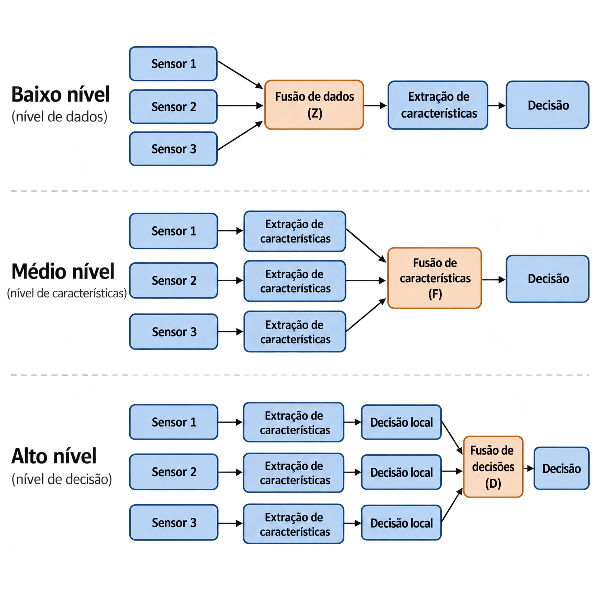
\includegraphics[width=0.85\textwidth]{figuras/fig_niveis_fusao.pdf}
    \caption{Níveis de fusão sensorial: o mesmo encadeamento de três sensores,
    variando o ponto em que a fusão ocorre --- sobre os dados brutos ($Z$), sobre as
    características extraídas ($F$) ou sobre as decisões locais de cada sensor ($D$).}
    \legend{Fonte: Elaborada pelo autor com base em \citeonline{Costa2018ImplementacaoFusao}
    e \citeonline{Santos2023FusaoSensorial}.}
    \label{fig:niveis_fusao}
\end{figure}
A \autoref{fig:niveis_fusao} ilustra os níveis de fusão sensorial.




\subsubsection{Fusão de Baixo Nível (Nível de Dados)}

A fusão de baixo nível envolve a combinação direta dos sinais provenientes dos sensores antes de qualquer extração de características ou interpretação semântica:

\begin{equation}
Z_{fusão} = f(Z_1, Z_2, ..., Z_n)
\end{equation}

Onde $Z_i$ representa os dados brutos do sensor $i$, e $f$ é a função de fusão aplicada.

Exemplos incluem combinação de nuvens de pontos de múltiplos sensores \ac{LiDAR} e fusão de imagens de diferentes espectros (\ac{RGB} + infravermelho). A principal vantagem é a preservação de toda a informação original, mas requer maior capacidade computacional e pode ser sensível a problemas de sincronização temporal e calibração espacial entre sensores \cite{Schneider2018FusaoSensores}.

\subsubsection{Fusão de Médio Nível (Nível de Características)}

A fusão de médio nível opera sobre características extraídas dos dados sensoriais brutos:

\begin{equation}
F_{fusão} = g(F_1, F_2, ..., F_n)
\end{equation}

Onde $F_i$ representa o conjunto de características extraídas do sensor $i$, e $g$ é a função de fusão aplicada às características.

Este nível oferece um bom equilíbrio entre redução de dimensionalidade (e consequentemente de carga computacional) e preservação de informação relevante \cite{Grassi2006ArquiteturaHibrida}.

\subsubsection{Fusão de Alto Nível (Nível de Decisão)}

A fusão de alto nível combina decisões ou classificações já realizadas por algoritmos específicos para cada sensor:

\begin{equation}
D_{fusão} = h(D_1, D_2, ..., D_n)
\end{equation}

Onde $D_i$ representa a decisão ou classificação baseada no sensor $i$, e $h$ é a função de fusão aplicada às decisões.

Este nível requer menor largura de banda para comunicação entre subsistemas, mas pode perder informações importantes durante o processo de decisão individual de cada sensor \cite{Ramos2012AplicacaoTecnicas}.

\subsection{Técnicas de Fusão Sensorial}

\subsubsection{Filtro de Kalman e suas Variantes}

O Filtro de Kalman é uma das técnicas mais utilizadas para fusão sensorial, especialmente para estimação de estados em sistemas dinâmicos lineares com ruído gaussiano \cite{Neto2021FiltrosRadarLidar}. 

O fluxograma que representa o Filtro de Kalman para fusão de sensores na \autoref{fig:filtro_kalman} segue as principais etapas do algoritmo de forma cíclica. 

\begin{figure}[h]
    \centering
%% Figura refeita em 14/11/2026. A versao anterior trazia "FILTRO DE KALMAN" como uma
%% caixa do fluxo, no mesmo nivel de MEDICAO e CORRECAO -- o todo desenhado como parte.
%% O ciclo tambem nao fechava, e havia duas setas sem significado (ESTADO ESTIMADO para
%% ESTADO PREVISTO contornando a PREDICAO, e CORRECAO para a caixa do filtro).
    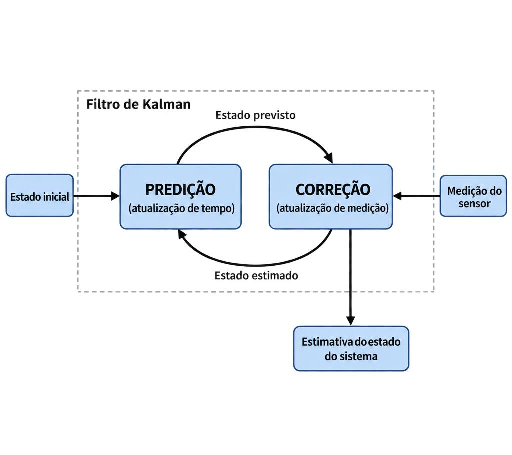
\includegraphics[width=0.8\textwidth]{figuras/fig_filtro_kalman.pdf}
    \caption{Ciclo do Filtro de Kalman: as duas fases, predição (atualização de tempo)
    e correção (atualização de medição), alternam-se indefinidamente, trocando entre si
    o estado previsto e o estado estimado. O filtro é o ciclo, não uma de suas etapas.}
    \legend{Fonte: Elaborada pelo autor.}
    \label{fig:filtro_kalman}
\end{figure}

Para cada etapa temos:

%% Reescrita em 14/11/2026, junto com a figura. A enumeracao anterior tinha tres
%% defeitos: (i) o item 1 dizia que a medicao "nao esta explicitamente rotulada" na
%% figura, o que deixou de ser verdade; (ii) o item 6 listava "Ciclo Recursivo do
%% Filtro de Kalman" como se fosse mais uma etapa, repetindo no texto o erro
%% categorico que a figura antiga cometia -- o ciclo e o conjunto, nao uma etapa; e
%% (iii) a ordem (medicao, correcao, estado estimado, predicao, estado previsto) nao
%% correspondia ao ciclo canonico de duas fases agora desenhado.
\begin{enumerate}
    \item \textbf{Predição (atualização de tempo).} Com base no modelo do sistema --- por exemplo, o modelo de movimento do robô ---, o filtro projeta o estado provável no instante seguinte, propagando também a incerteza associada ao processo. Seu resultado é o \emph{estado previsto}.

    \item \textbf{Medição do sensor.} Chega uma nova observação dos sensores (\ac{IMU}, GPS, \ac{LiDAR}, entre outros), que alimenta a etapa de correção. Ao contrário do estado previsto, ela é informação externa ao modelo.

    \item \textbf{Correção (atualização de medição).} Compara-se a medição com o estado previsto. Da comparação resulta o ganho de Kalman, que pondera quanto o filtro deve confiar na medição atual em relação à previsão. O resultado é o \emph{estado estimado}, melhor estimativa corrente das variáveis de estado: posição, velocidade e demais.

    \item \textbf{Realimentação.} O estado estimado retorna à predição, que projeta o instante seguinte, e o ciclo recomeça. Note-se que o filtro \emph{é} esse ciclo: predição e correção alternam-se indefinidamente, e não existe uma etapa separada à qual caiba o nome de filtro de Kalman.
\end{enumerate}

O Filtro de Kalman é amplamente usado em fusão sensorial para, combinar medições ruidosas e incompletas de múltiplos sensores, obter uma estimativa mais confiável do estado do sistema e também para operar de forma online, ajustando-se em tempo real à medida que novas medições chegam.


Na etapa de predição, o estado atual é estimado com base no estado anterior e no modelo do sistema:

\begin{equation}
\hat{x}_{k|k-1} = F_k\hat{x}_{k-1|k-1} + B_ku_k
\end{equation}

\begin{equation}
P_{k|k-1} = F_kP_{k-1|k-1}F_k^T + Q_k
\end{equation}

Na etapa de atualização, a estimativa é corrigida com base nas medições dos sensores:

\begin{equation}
K_k = P_{k|k-1}H_k^T(H_kP_{k|k-1}H_k^T + R_k)^{-1}
\end{equation}

\begin{equation}
\hat{x}_{k|k} = \hat{x}_{k|k-1} + K_k(z_k - H_k\hat{x}_{k|k-1})
\end{equation}

Para sistemas não-lineares, variantes como o Filtro de Kalman Estendido (\ac{EKF}) e o Filtro de Kalman Unscented (\ac{UKF}) são utilizadas \cite{Costa2018ImplementacaoFusao}.

\subsubsection{Redes Bayesianas}

As redes Bayesianas oferecem um \textit{framework} probabilístico para modelar relações causais entre variáveis, sendo particularmente úteis para fusão sensorial de alto nível \cite{Ramos2012AplicacaoTecnicas}. A probabilidade conjunta de todas as variáveis na rede é dada por:

\begin{equation}
P(X_1, X_2, ..., X_n) = \prod_{i=1}^{n} P(X_i | Pa(X_i))
\end{equation}

Onde $Pa(X_i)$ representa o conjunto de pais do nó $X_i$ no grafo.

Em fusão sensorial, as redes Bayesianas permitem integrar informações de diferentes sensores considerando suas incertezas e relações causais.

\subsubsection{Redes Neurais e Aprendizado Profundo}

Técnicas de aprendizado de máquina, especialmente redes neurais profundas, têm sido cada vez mais aplicadas para fusão sensorial \cite{Wu2022LidarFusionSurvey, Ou2024SensorFusionDRL}. Estas abordagens permitem aprender automaticamente representações e relações complexas entre diferentes modalidades sensoriais.

Arquiteturas comuns incluem Redes Neurais Convolucionais (\ac{CNN}) para processamento de dados espaciais, Redes Neurais Recorrentes (\ac{RNN}) para sequências temporais, e arquiteturas multimodais específicas para combinar diferentes tipos de dados sensoriais.

Uma arquitetura típica de fusão sensorial baseada em aprendizado profundo pode ser representada como:

\begin{equation}
F_{fusão} = f_{fusão}(f_1(X_1), f_2(X_2), ..., f_n(X_n))
\end{equation}

Onde $X_i$ representa os dados do sensor $i$, $f_i$ é a rede neural específica para processar o sensor $i$, e $f_{fusão}$ é a rede de fusão que combina as representações intermediárias.

\subsection{Desafios da Fusão em Ambientes com Interferência Eletromagnética}

A fusão sensorial em subestações elétricas enfrenta desafios específicos devido à
presença de campos eletromagnéticos intensos \cite{He2007EMCSubstation, Yan2024CombinedNav}.
O campo induz ruído e distorção nos próprios sensores eletrônicos, e os magnéticos, os
inerciais e os de comunicação sem fio são os mais suscetíveis. A intensidade e a
distribuição espacial dessa interferência variam ao longo do tempo, de modo que um
conjunto fixo de pesos entre sensores não se sustenta por toda a missão. E a degradação
não é uniforme: cada modalidade é afetada de maneira distinta, o que transfere o problema
da filtragem de um sinal para a estratégia de fusão, que precisa decidir qual leitura
desacreditar e quando. Técnicas de mitigação incluem blindagem eletromagnética, filtragem
digital e algoritmos de detecção e compensação de interferência \cite{Yan2024CombinedNav}.

\subsection{Modelos de Pesos e Bias para Relevância Sensorial}

A ponderação relativa entre sensores determina o resultado da fusão, e precisa refletir a confiabilidade, a relevância e a qualidade momentânea de cada leitura \cite{Neto2021FiltrosRadarLidar, Schneider2018FusaoSensores}.

\subsubsection{Ponderação Baseada em Covariância}

Um método comum para atribuir pesos aos sensores é baseado na matriz de covariância do erro de medição. Sensores com menor incerteza (menor covariância) recebem maior peso. Para o caso de fusão de estimativas escalares de múltiplos sensores, a estimativa ótima é dada por:

\begin{equation}
\hat{x} = \sum_{i=1}^{n} w_i x_i
\end{equation}

Onde os pesos $w_i$ são calculados como:

\begin{equation}
w_i = \frac{\sigma_i^{-2}}{\sum_{j=1}^{n} \sigma_j^{-2}}
\end{equation}

Com $\sigma_i^2$ representando a variância do erro de medição do sensor $i$.

\subsubsection{Ponderação Adaptativa Baseada em Contexto}

Em ambientes dinâmicos como subestações elétricas, a confiabilidade dos sensores pode variar em função do contexto operacional. Modelos adaptativos de ponderação consideram fatores contextuais para ajustar os pesos dos sensores em tempo real \cite{Yan2024CombinedNav}:

\begin{equation}
w_i(t) = f_w(w_i^{base}, c_1(t), c_2(t), ..., c_m(t))
\end{equation}

Onde $w_i(t)$ é o peso do sensor $i$ no instante $t$, $w_i^{base}$ é o peso base do sensor $i$, $c_j(t)$ são fatores contextuais (nível de interferência eletromagnética, iluminação, etc.), e $f_w$ é a função de adaptação dos pesos.

\subsection{Aplicações em Robótica Móvel para Inspeção}

A fusão sensorial heterogênea é particularmente relevante para robôs de inspeção em
subestações elétricas, onde diferentes tipos de sensores são necessários para detectar
diversos tipos de anomalias \cite{Lactec2022, Iberdrola2022}. A detecção de pontos
quentes combina imagem térmica com imagem visual, porque a térmica localiza o excesso de
temperatura e a visual identifica em qual componente ele está. A de descargas parciais
combina sensores acústicos, \ac{UV} e \ac{RF}, nenhum dos quais localiza a descarga
isoladamente. A navegação sob interferência eletromagnética recorre a \ac{LiDAR}, câmeras
e \ac{IMU} em conjunto, pela mesma razão que motiva a ponderação adaptativa da subseção
anterior. E a inspeção visual de corrosão, dano físico e vazamento combina as modalidades
visual, térmica e \ac{UV}, que expõem defeitos de naturezas diferentes na mesma
superfície.

Nenhuma das técnicas de fusão descritas acima é implementada nesta tese. Elas delimitam o que se entende por evento sensorial na Seção~\ref{sec:prop-sensoriamento}, onde a detecção entra no sistema já classificada por modalidade e intensidade, e o objeto de estudo passa a ser a decisão que vem depois dela.

%% Listas convertidas em prosa em 15/11/2026: 12 de 14. As duas mantidas sao
%% GLOSSARIOS DE NOTACAO imediatamente apos a definicao a que se referem (as
%% componentes da tupla do MDP e os termos da regra de atualizacao do Q). Isso e
%% convencao matematica, nao lista didatica: converter em prosa corrida piora a
%% consulta, que e a funcao delas.
%% Revisao estilistica em 15/11/2026. Reescritos a abertura e o paragrafo de
%% fechamento. O fecho anterior afirmava o "potencial do aprendizado por
%% reforco como componente fundamental" da proposta -- promessa da
%% qualificacao que a avaliacao nao sustenta. Ele agora declara o contrario,
%% que a camada principal arbitra por limiar deterministico, e diz por que.
\section{Aprendizado por Reforço}
\label{sec:fund-rl}

O Aprendizado por Reforço (\textit{Reinforcement Learning}, RL) aprende uma política por interação com o ambiente, sem exemplos rotulados de ação correta. Esta seção percorre seus elementos formais, os algoritmos relevantes para controle robótico e as razões pelas quais a camada principal desta tese não adota uma política aprendida. 

\subsection{Fundamentos do Aprendizado por Reforço}

O aprendizado por reforço é um paradigma onde um agente aprende a tomar decisões sequenciais através de interações com um ambiente, recebendo recompensas ou penalidades como feedback \cite{Sutton2018}. Diferentemente do aprendizado supervisionado ou não-supervisionado, o aprendizado por reforço foca na maximização de uma recompensa cumulativa ao longo do tempo \cite{Arulkumaran2017DeepRL}. A \autoref{fig:agente_ambiente} mostra o ciclo de interação entre o agente e o ambiente no aprendizado por reforço.

\begin{figure}[h]
    \centering
%% Figura refeita em 14/11/2026. A versao anterior omitia o ESTADO -- elemento central
%% do paradigma, listado logo abaixo e presente em toda a formalizacao do MDP -- e
%% trazia uma segunda seta do agente para o ambiente, horizontal e sem rotulo nenhum.
    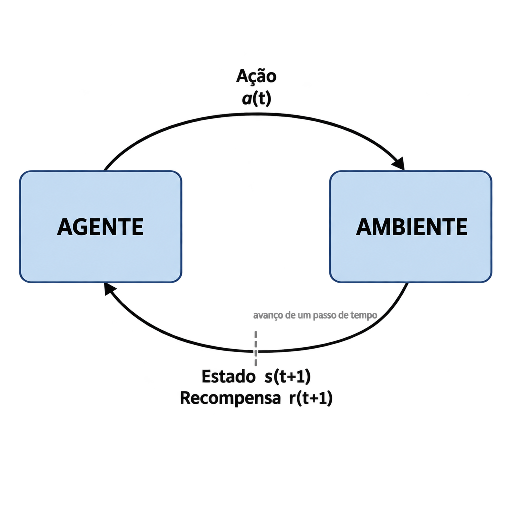
\includegraphics[width=0.8\textwidth]{figuras/fig_agente_ambiente.pdf}
    \caption{Ciclo de interação agente--ambiente no aprendizado por reforço. O agente
    emite a ação $a(t)$; o ambiente devolve o novo estado $s(t+1)$ e a recompensa
    $r(t+1)$, com o avanço de um passo de tempo assinalado sobre a seta de retorno.}
    \legend{Fonte: Elaborada pelo autor com base em \citeonline{Sutton2018}.}
    \label{fig:agente_ambiente}
\end{figure}


\subsubsection{Elementos Fundamentais}

O framework do aprendizado por reforço é composto por cinco elementos
\cite{Sutton2018}. O \emph{agente} é a entidade que decide e aprende, um robô autônomo
no caso que interessa aqui, e o \emph{ambiente} é o mundo com que ele interage, a
subestação. O \emph{estado} $s \in S$ representa a situação corrente de ambos; a
\emph{ação} $a \in A$ é a decisão do agente, capaz de alterar essa situação; e a
\emph{recompensa} $r \in \mathbb{R}$ é um escalar que informa o sucesso imediato da ação
executada. Toda a dificuldade do paradigma está nesse último elemento, porque um escalar
por passo é um canal estreito para comunicar o que se quer de um comportamento.

\subsubsection{Processo de Decisão de Markov}

O aprendizado por reforço é frequentemente formalizado como um Processo de Decisão de Markov (MDP), definido pela tupla $(S, A, P, R, \gamma)$ \cite{Puterman2014}:

\begin{itemize}
    \item $S$ é o conjunto de estados possíveis.
    \item $A$ é o conjunto de ações possíveis.
    \item $P: S \times A \times S \rightarrow [0, 1]$ é a função de transição de estados.
    \item $R: S \times A \times S \rightarrow \mathbb{R}$ é a função de recompensa.
    \item $\gamma \in [0, 1]$ é o fator de desconto, que determina a importância de recompensas futuras.
\end{itemize}

A propriedade de Markov estabelece que o próximo estado e a recompensa dependem apenas do estado atual e da ação tomada, não da história completa de estados e ações anteriores.

\subsubsection{Política e Função Valor}

O objetivo do agente é aprender uma política ótima $\pi^*: S \rightarrow A$ que maximize a recompensa cumulativa esperada. A política $\pi$ mapeia estados para ações (ou distribuições de probabilidade sobre ações) \cite{Sutton2018}.

A recompensa cumulativa descontada a partir do estado $s$ seguindo a política $\pi$ é definida como:

\begin{equation}
G_t = \sum_{k=0}^{\infty} \gamma^k R_{t+k+1}
\end{equation}

Duas funções são usadas para avaliar políticas. A \emph{função valor de estado}
$V^{\pi}$ dá o valor esperado de seguir a política $\pi$ a partir do estado $s$,

\begin{equation}
V^{\pi}(s) = \mathbb{E}_{\pi}[G_t | S_t = s]
\end{equation}

enquanto a \emph{função valor de ação} $Q^{\pi}$ dá o valor esperado de executar a ação
$a$ no estado $s$ e só então seguir $\pi$,

\begin{equation}
Q^{\pi}(s, a) = \mathbb{E}_{\pi}[G_t | S_t = s, A_t = a]
\end{equation}

distinção que importa porque é sobre a segunda, e não sobre a primeira, que se pode
decidir uma ação sem conhecer a dinâmica do ambiente.

\subsection{Algoritmo Q-Learning e Variantes}

O Q-Learning é um dos algoritmos mais fundamentais e amplamente utilizados no aprendizado por reforço, especialmente em aplicações robóticas \cite{Watkins1992}.

\subsubsection{Q-Learning Clássico}

O Q-Learning é um algoritmo livre de modelo (\textit{model-free}) que aprende diretamente a função valor ótima $Q^*$ sem necessidade de conhecer a dinâmica do ambiente \cite{Watkins1992}.

O algoritmo atualiza iterativamente a estimativa da função $Q$ usando a seguinte regra:

\begin{equation}
Q(s_t, a_t) \leftarrow Q(s_t, a_t) + \alpha [r_{t+1} + \gamma \max_{a} Q(s_{t+1}, a) - Q(s_t, a_t)]
\label{eq:fund-qlearning}
\end{equation}

Onde:
\begin{itemize}
    \item $\alpha \in (0, 1]$ é a taxa de aprendizado.
    \item $r_{t+1}$ é a recompensa recebida após executar a ação $a_t$ no estado $s_t$.
    \item $\gamma$ é o fator de desconto.
    \item $\max_{a} Q(s_{t+1}, a)$ é o valor máximo estimado para o próximo estado $s_{t+1}$.
\end{itemize}

%% Acrescentado em 15/11/2026. O capitulo ensinava a regra de atualizacao sem nomear a
%% equacao de Bellman, e a Secao 4.6 fala da "equacao de Bellman" e rotula sua equacao
%% como eq:prop-bellman. "Bellman" ocorria ZERO vezes em todo o Capitulo 2 e 3 vezes
%% nos capitulos posteriores: o leitor encontrava o nome depois do uso.
A expressão entre colchetes na Equação~\eqref{eq:fund-qlearning} é o \emph{erro de
diferença temporal}: a discrepância entre o valor estimado para o par corrente e a
estimativa revista à luz da recompensa observada e do melhor valor disponível no estado
seguinte. A regra desloca a estimativa na direção dessa discrepância, numa fração
$\alpha$ dela. O ponto fixo dessa iteração é a \emph{equação de Bellman} de otimalidade,
\begin{equation}
Q^*(s,a) = \mathbb{E}\!\left[\, r + \gamma \max_{a'} Q^*(s',a') \,\right],
\label{eq:fund-bellman}
\end{equation}
que caracteriza a função valor ótima por uma condição de consistência: o valor de um par
estado-ação é a recompensa imediata esperada mais o valor descontado do melhor que se pode
fazer em seguida. Não é uma regra de cálculo, e sim a identidade que a solução satisfaz; o
Q-Learning é um dos procedimentos que convergem para ela. Essa distinção entre a
\emph{identidade} e o \emph{procedimento} será retomada no
Capítulo~\ref{cap:proposta}, onde se discute o que significa acrescentar um termo à
atualização sem alterar a identidade que ela persegue.

Uma característica importante do Q-Learning é o dilema exploração-explotação: o agente precisa balancear entre explorar novas ações (para descobrir melhores estratégias) e explotar o conhecimento atual (para maximizar recompensas). A estratégia $\epsilon$-greedy é comumente utilizada, onde com probabilidade $\epsilon$, escolhe-se uma ação aleatória (exploração); caso contrário, escolhe-se a ação com maior valor Q (explotação).

\subsubsection{Variantes do Q-Learning}

\paragraph{SARSA}

SARSA (State-Action-Reward-State-Action) é uma variante do Q-Learning que utiliza a política atual para atualizar os valores Q \cite{Rummery1994}. A regra de atualização é:

\begin{equation}
Q(s_t, a_t) \leftarrow Q(s_t, a_t) + \alpha [r_{t+1} + \gamma Q(s_{t+1}, a_{t+1}) - Q(s_t, a_t)]
\end{equation}

A principal diferença entre Q-Learning e SARSA é que o Q-Learning é um algoritmo \textit{off-policy} (aprende a política ótima independentemente da política de exploração), enquanto SARSA é \textit{on-policy} (aprende a política que está sendo seguida).

\paragraph{Double Q-Learning}

O Double Q-Learning foi proposto para mitigar o problema de superestimação presente no Q-Learning tradicional \cite{Hasselt2010}. O algoritmo mantém duas funções valor, $Q_A$ e $Q_B$, e utiliza uma para selecionar ações e outra para avaliá-las, reduzindo o viés de superestimação.

%% Secao COMPRIMIDA e ACRESCIDA em 15/11/2026. Antes: 317 palavras sobre DQN e
%% algoritmos de politica, com figura propria, e NADA sobre moldagem de recompensa.
%% O desequilibrio era mensuravel: "DQN" ocorria 6 vezes aqui e zero nos Capitulos 4
%% a 7, enquanto `shaping' e `invariancia de politica' ocorriam ZERO aqui e 3 vezes na
%% Secao 4.7, onde esta tese declara que seu campo NAO tem a forma potencial de Ng. O
%% leitor precisava ja saber o que e essa garantia para entender o que estava sendo
%% renunciado. O DQN foi mantido em forma curta porque o Capitulo 3 depende dele (13
%% ocorrencias de DRL/DQN la), mas a figura fig_dqn saiu: ela detalhava rede alvo e
%% buffer de repeticao, que nenhum capitulo posterior usa.
\subsection{Aprendizado por Reforço Profundo}

O aprendizado por reforço profundo substitui a tabela de valor por um aproximador
paramétrico, o que o torna aplicável a espaços de estado de alta dimensão onde a tabela
seria intratável \cite{Arulkumaran2017DeepRL}. A \textit{Deep Q-Network} aprende
$Q(s,a;\theta)$ com uma rede neural em lugar de uma entrada por par estado-ação
\cite{Mnih2015}, e as duas técnicas que a tornaram treinável atacam a mesma dificuldade,
a correlação entre amostras consecutivas: a repetição de experiências treina a rede com
mini-lotes sorteados de um \textit{buffer} de transições, quebrando a ordem temporal, e a
rede alvo mantém uma segunda cópia de parâmetros atualizada apenas periodicamente, de
sorte que o alvo da regressão não se desloca a cada passo junto com a rede que o persegue.
Uma segunda família aprende a política diretamente, em vez de derivá-la de uma função
valor \cite{Sutton1999}: os métodos \textit{actor-critic} acoplam um aprendiz de política
a um de valor \cite{Konda1999}, e o \ac{PPO} limita a magnitude de cada atualização para
estabilizar o treino \cite{Schulman2017}. Nenhuma dessas famílias é empregada nesta tese,
que opera com tabela de valor discreta; elas aparecem aqui porque a literatura revisada no
Capítulo~\ref{cap:revisao} é majoritariamente construída sobre elas.

\subsection{Moldagem de Recompensa e Invariância de Política}
\label{sec:fund-shaping}

Recompensa esparsa torna o aprendizado lento: se o sinal só chega ao alcançar o objetivo,
o agente precisa encontrá-lo por exploração antes de ter o que aprender. A \emph{moldagem
de recompensa} acrescenta à recompensa original $r$ um termo $F$ que oferece sinal
intermediário, de modo que o agente aprende sobre a soma $r+F$ em vez de sobre $r$. O
expediente é antigo e eficaz, mas introduz um risco que lhe é próprio: um termo mal
escolhido pode deslocar a política ótima, premiando um comportamento que acumula $F$ sem
cumprir a tarefa --- o caso extremo é o agente que circula indefinidamente entre estados
de alto $F$ em vez de terminar.

\citeonline{ng1999} delimitaram exatamente quando esse risco não existe. O resultado é que
$F$ preserva a política ótima para \emph{qualquer} recompensa original se e somente se
tiver a forma \emph{potencial}
\begin{equation}
F(s,a,s') = \gamma\,\Phi(s') - \Phi(s),
\label{eq:fund-shaping}
\end{equation}
isto é, se for a diferença descontada de uma função $\Phi$ sobre estados. A propriedade
tem nome: \emph{invariância de política} sob transformação de recompensa. A intuição é que
um termo dessa forma se cancela ao longo de qualquer trajetória fechada, de sorte que
nenhum ciclo acumula recompensa artificial, e o que ele altera é a velocidade do
aprendizado, não o seu destino.

A distinção importa porque fixa o ônus da prova. Um termo aditivo que \emph{não} assuma a
forma da Equação~\eqref{eq:fund-shaping} --- por ser variante no tempo, por depender de
evento observado ou por somar-se diretamente ao valor em vez de entrar como diferença de
potencial --- não herda garantia alguma, e qualquer afirmação sobre a política resultante
precisa ser demonstrada caso a caso. A Seção~\ref{sec:prop-atualizacao} retoma esse
ponto para declarar o estatuto do campo formulado nesta tese, que é precisamente um termo
dessa segunda espécie.
\subsection{Aplicações em Robótica Autônoma}

O aprendizado por reforço tem sido aplicado em robótica autônoma sobretudo em percepção, navegação e manipulação \cite{Kober2013}.

\subsubsection{Navegação Autônoma}

A navegação autônoma é uma das aplicações mais relevantes do aprendizado por reforço em robótica, especialmente em ambientes dinâmicos e não estruturados como subestações elétricas \cite{Faria2002}.

Para um robô móvel, o problema de navegação pode ser formulado como um MDP em que os
estados são representações da posição, da orientação e da percepção sensorial do robô, as
ações são comandos de movimento, tipicamente velocidades linear e angular, e as
recompensas são positivas na aproximação ao objetivo e negativas em colisões e em
comportamentos indesejados. É na terceira dessas escolhas que se concentra o trabalho de
projeto, porque ela precisa codificar, num escalar, tudo o que distingue uma trajetória
aceitável de uma inaceitável.

As abordagens de aprendizado por reforço aplicadas à navegação robótica distinguem-se
pelo que supõem sobre o mapa. A navegação \emph{baseada em mapas} aprende a se deslocar
sobre uma representação do ambiente, frequentemente combinando aprendizado com técnicas
de SLAM. A navegação \emph{reativa} dispensa o mapa explícito e aprende a responder
diretamente às percepções sensoriais \cite{Zhu2017,Tai2017}.
%% Corrigido em 14/11/2026 (auditoria bibliografica): Tai2017 sustentava o item de
%% navegacao baseada em mapas, mas o proprio titulo do trabalho e "continuous control
%% of mobile robots for MAPLESS navigation" -- e a categoria oposta. A citacao foi
%% retirada daquele item (a categoria e descritiva e nao precisa de apoio pontual) e
%% passada ao item reativo, onde descreve corretamente a fonte.
A navegação \emph{hierárquica} combina as duas, com planejamento de alto nível sobre
controle reativo de baixo nível \cite{Kulkarni2016}, e é a essa terceira família que a
arquitetura desta tese se filia, com a diferença de que a camada de alto nível aqui não
é aprendida.

\subsubsection{Inspeção Autônoma}

%% Reescrito em 13/11/2026 (auditoria bibliografica): a referencia anterior desta
%% frase nao foi localizada em nenhuma base. A alegacao de aplicacao bem-sucedida de
%% aprendizado por reforco a inspecao de subestacoes foi retirada; o que a literatura
%% verificada sustenta e o uso de aprendizado em navegacao sobre observacoes fundidas,
%% em robotica movel, e nao em inspecao de subestacao em operacao.
O aprendizado por reforço tem sido aplicado a tarefas de navegação autônoma sobre observações sensoriais fundidas \cite{Ou2024SensorFusionDRL}; sua transposição para a inspeção de infraestruturas críticas como subestações elétricas permanece, em larga medida, uma direção em aberto.

Em aplicações de inspeção, o aprendizado por reforço pode ser empregado no planejamento
de trajetórias que maximizem cobertura e qualidade, na detecção e investigação de
anomalias encontradas durante a ronda, e na adaptação do comportamento a condições
ambientais variáveis. As três tarefas diferem em horizonte: a primeira é decidida antes
da missão, a segunda durante, e a terceira ao longo de missões sucessivas.

\subsection{Desafios e Limitações}

%% Reescrito em 15/11/2026. A frase abria por "Apesar de seu potencial" e terminava em
%% dois-pontos, mas o que vinha depois era um \subsubsection: os dois-pontos nao
%% anunciavam nada. As tres restricoes nomeadas sao exatamente as tres subsecoes.
A transposição do aprendizado por reforço de jogos e de ambientes de teste simulados para o robô físico esbarra em três restrições operacionais \cite{Kober2013, Arulkumaran2017DeepRL}, tratadas nas três subseções seguintes.

\subsubsection{Eficiência de Amostra}

O aprendizado por reforço frequentemente requer um grande número de interações com o
ambiente para aprender políticas eficazes, o que é impraticável em robótica real pelo
tempo e pelo desgaste envolvidos. As mitigações usuais deslocam o custo em vez de
removê-lo: treinar em simulação antes de transferir para o mundo real troca interações
reais por uma lacuna de domínio a vencer; inicializar a política com demonstrações
humanas ou de outro sistema troca-as pela qualidade do que se demonstrou; e reutilizar
conhecimento de tarefas anteriores troca-as pela semelhança entre as tarefas, que precisa
ser verdadeira.

\subsubsection{Exploração Segura}

Em robótica, a exploração aleatória pode levar a comportamentos que danificam o robô ou o
ambiente, e os métodos de exploração segura diferem em onde colocam a restrição. A
exploração guiada por incerteza a coloca na escolha da próxima ação, dirigindo-a para
onde o agente sabe menos. As restrições de segurança a colocam na formulação do problema
ou na função de recompensa, antes do aprendizado. E as formulações com risco limitado a
colocam no critério otimizado, que passa a penalizar explicitamente a cauda ruim em vez
da média. Nesta tese a restrição está em outro lugar ainda: fora da política, numa regra
de precedência que o aprendizado não pode negociar.

\subsubsection{Generalização e Transferência}

Políticas aprendidas em um ambiente ou configuração específica frequentemente não
generalizam para novos, e os três obstáculos reconhecidos são de naturezas distintas. A
transferência \textit{sim-to-real} enfrenta uma diferença sistemática entre o simulador e
o mundo. A adaptação a ambientes não vistos no treinamento enfrenta uma diferença entre
instâncias do mesmo tipo de ambiente. E a robustez a perturbações enfrenta variação
dentro de uma única instância, durante a operação. Confundir as três faz um resultado de
simulação parecer uma garantia de campo.

\subsection{Integração com Outros Paradigmas}

Para superar as limitações do aprendizado por reforço puro, abordagens híbridas que integram outros paradigmas têm sido propostas \cite{Kober2013}:

\subsubsection{Integração com Controle Clássico}

A combinação de aprendizado por reforço com controle clássico admite três arranjos, que
diferem em qual dos dois tem a palavra final. Modelos aprendidos podem alimentar
controladores clássicos, melhorando-lhes a predição sem alterar a estrutura de controle.
Controladores clássicos podem guiar a exploração durante o aprendizado, restringindo o
que o agente chega a experimentar. E arquiteturas híbridas podem reservar as tarefas
críticas de segurança ao controlador clássico e deixar à política aprendida apenas a
otimização de desempenho, que é a divisão de responsabilidade mais próxima da adotada no
Capítulo~\ref{cap:proposta}.

\subsubsection{Integração com Planejamento Simbólico}

A integração de aprendizado por reforço com planejamento simbólico atende a tarefas de
longo prazo por três vias. Hierarquias de abstração reservam o alto nível ao planejamento
simbólico e a execução ao aprendizado. Representações simbólicas facilitam transferir
conhecimento entre tarefas, porque descrevem a tarefa em termos que sobrevivem à troca de
ambiente. E conhecimento causal explícito melhora a eficiência do aprendizado e a
interpretabilidade da política resultante, que é precisamente o que falta às políticas
puramente aprendidas quando se exige certificação.

\subsection{Aplicações Específicas em Subestações Elétricas}

A literatura aponta quatro usos do aprendizado por reforço na inspeção autônoma de
subestações \cite{Ou2024SensorFusionDRL, Wei2024Advancements}: aprender políticas de
navegação que se adaptem à interferência eletromagnética variável; aprender a priorizar
equipamentos por criticidade, histórico de falhas e indicadores de anomalia; aprender a
investigar a anomalia detectada, ajustando o comportamento para coletar informação
adicional quando necessário; e ajustar a estratégia de inspeção a condições de
iluminação, clima e interferência. Os quatro supõem que a decisão a ser aprendida seja a
decisão de inspeção, e é exatamente essa suposição que esta tese não adota.

A camada principal desta tese não usa política aprendida. O arbítrio entre inspecionar e se afastar é resolvido por limiar determinístico (Capítulo~\ref{cap:proposta}), escolha que decorre de duas das limitações expostas acima, a eficiência de amostra e a opacidade da política treinada; a tabela \textit{Q} comparece no trabalho como linha de base comparativa (Seção~\ref{sec:setup-qdriven}).

\section{Inspeção em Subestação de Energia Elétrica}

As subestações de energia elétrica representam componentes críticos do sistema elétrico de potência, responsáveis pela transformação, distribuição e controle da energia elétrica. Esta seção apresenta os fundamentos teóricos relacionados às subestações elétricas, métodos de inspeção e aplicações de sistemas robóticos neste contexto.

\subsection{Fundamentos de Subestações Elétricas}
\begin{figure}[h!]
    \centering
%% Figura refeita em 14/11/2026. Na versao anterior o rotulo "Transformador de
%% potencia" aparecia DUAS vezes apontando para objetos diferentes; o rotulo
%% "Barramentos" apontava para uma interligacao em vez do barramento principal; um ramo
%% inteiro ficava sem identificacao; e o para-raios estava em serie na linha, com um
%% aterramento no meio da propria linha principal -- eletricamente, um curto.
    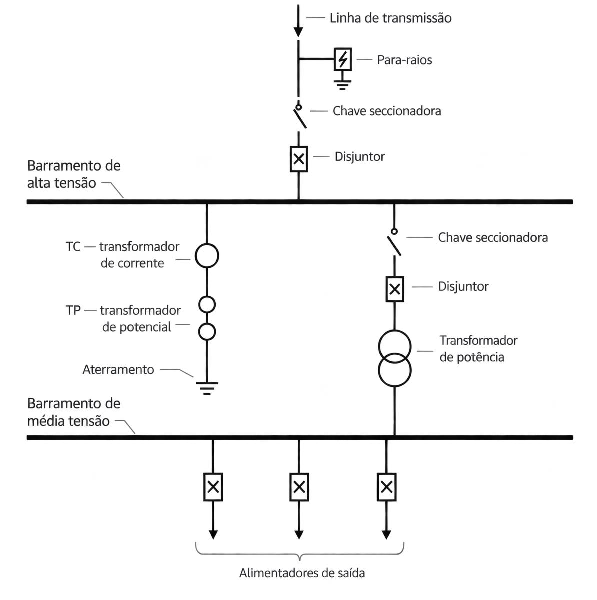
\includegraphics[width=0.8\textwidth]{figuras/fig_subestacao_tipica.pdf}
    \caption{Diagrama unifilar simplificado de uma subestação elétrica típica, da linha
    de transmissão aos alimentadores de saída, com o vão de medição (TC e TP) e o vão de
    transformação derivados do barramento de alta tensão.}
    \legend{Fonte: Adaptado de \citeonline{Muzy2012}.}
    \label{fig:subestacao_tipica}
\end{figure}

Subestações elétricas são instalações que contêm equipamentos para transmissão e distribuição de energia elétrica, além de equipamentos de proteção, medição e controle \cite{Muzy2012}. Elas desempenham funções essenciais no sistema elétrico, incluindo transformação de tensão, seccionamento de linhas, compensação de reativos e interligação de sistemas \cite{Kindermann2012}.

\subsubsection{Classificação e Componentes Principais}

As subestações podem ser classificadas segundo diversos critérios \cite{Mamede2017}:

\begin{itemize}
    \item \textbf{Quanto à função}: Elevadoras, abaixadoras, seccionadoras e de manobra.
    \item \textbf{Quanto ao nível de tensão}: Baixa tensão (até 1 kV), média tensão (1-36,2 kV), alta tensão (36,2-230 kV), extra-alta tensão (acima de 230 kV) e ultra-alta tensão (acima de 800 kV).
    \item \textbf{Quanto ao tipo de instalação}: Convencionais, abrigadas, blindadas, subterrâneas e móveis.
\end{itemize}

Os principais componentes de uma subestação incluem \cite{Frontin2013}:

\begin{itemize}
    \item \textbf{Transformadores de potência}: Responsáveis pela transformação dos níveis de tensão.
    \item \textbf{Equipamentos de manobra}: Disjuntores e chaves seccionadoras.
    \item \textbf{Transformadores de instrumentação}: TCs e TPs para medição e proteção.
    \item \textbf{Equipamentos de proteção}: Para-raios, relés e sistemas de aterramento.
    \item \textbf{Sistemas de controle e supervisão}: SCADA e dispositivos eletrônicos inteligentes (IEDs).
\end{itemize}

O arranjo de barramentos define a configuração física e elétrica da subestação, impactando sua confiabilidade, flexibilidade operativa e custo. Os principais arranjos incluem barra simples, barra principal e transferência, barra dupla, disjuntor e meio, e configuração em anel \cite{Frontin2013}.

\subsection{Normas Técnicas e Regulamentação}

As subestações elétricas são regidas por um conjunto abrangente de normas técnicas e regulamentações que visam garantir a segurança, confiabilidade e padronização das instalações \cite{ABNT2021}. No Brasil, destacam-se as normas ABNT NBR 14039 (média tensão), NBR 5410 (baixa tensão) e NBR 5419 (proteção contra descargas atmosféricas).

Internacionalmente, as normas IEC 61936-1, IEC 62271, IEC 60076 e IEC 61850 estabelecem padrões para instalações de alta tensão, equipamentos de manobra, transformadores e comunicação em subestações, respectivamente \cite{ABNT2021}.

O setor elétrico brasileiro é regulado pela ANEEL (regulação e fiscalização), ONS (operação do sistema), EPE (planejamento) e CCEE (comercialização), com os Procedimentos de Rede do ONS estabelecendo requisitos mínimos para subestações \cite{ONS2020}.

\subsection{Métodos Tradicionais de Inspeção}

A inspeção de subestações elétricas é fundamental para garantir a confiabilidade, segurança e eficiência do sistema elétrico. Tradicionalmente, estas inspeções são realizadas por técnicos especializados, seguindo procedimentos e periodicidades estabelecidos em normas e manuais de manutenção \cite{Silva2019}.

\subsubsection{Principais Métodos}

Os métodos tradicionais de inspeção incluem:

\begin{itemize}
    \item \textbf{Inspeção Visual}: Observação direta dos equipamentos para identificar vazamentos, danos físicos, conexões soltas, trincas em isoladores e outros problemas visíveis \cite{Inovarum2017}.
    
    \item \textbf{Ensaios Elétricos}: Medições de resistência de isolamento, resistência de contato, relação de transformação, fator de potência e testes funcionais de proteção \cite{Conprove2019}.
    
    \item \textbf{Análises Físico-Químicas}: Avaliação de propriedades do óleo isolante, análise de gases dissolvidos e compostos furânicos para equipamentos como transformadores e disjuntores \cite{Inovarum2017}.
    
    \item \textbf{Termografia}: Identificação de pontos de aquecimento anormal através de câmeras termográficas, indicativos de problemas como maus contatos ou sobrecargas \cite{Pixforce2024}.
    
    \item \textbf{Medição de Descargas Parciais}: Detecção de falhas incipientes em isolação elétrica através de métodos acústicos, elétricos ou UHF \cite{Frontin2013}.
\end{itemize}

\subsubsection{Limitações dos Métodos Tradicionais}

Apesar de sua eficácia, os métodos tradicionais apresentam limitações significativas \cite{GlobalGrowthInsights2024}:

\begin{itemize}
    \item \textbf{Exposição a riscos}: Os técnicos estão expostos a riscos elétricos, mecânicos e ambientais.
    \item \textbf{Necessidade de desligamento}: Muitos ensaios requerem o desligamento dos equipamentos.
    \item \textbf{Subjetividade}: A interpretação dos resultados pode variar conforme a experiência do inspetor.
    \item \textbf{Periodicidade limitada}: As inspeções são realizadas em intervalos predefinidos.
    \item \textbf{Custo elevado}: Inspeções manuais requerem mão de obra especializada.
    \item \textbf{Acesso limitado}: Alguns componentes são de difícil acesso para inspeção manual.
\end{itemize}

\subsection{Métodos Avançados e Automatizados de Inspeção}

Para superar as limitações dos métodos tradicionais, têm sido desenvolvidas técnicas avançadas e automatizadas de inspeção, que permitem monitoramento contínuo, maior segurança e detecção precoce de falhas \cite{Wei2024Advancements}.

\subsubsection{Monitoramento Online e Sistemas Integrados}

O monitoramento online permite a avaliação contínua do estado dos equipamentos sem necessidade de desligamento, utilizando sensores para gases dissolvidos em óleo, descargas parciais, temperatura, vibração e sinais acústicos \cite{Clouglobal2024}.

Sistemas de monitoramento integrados combinam diversos sensores e técnicas de análise, frequentemente utilizando comunicação baseada no padrão IEC 61850, que define protocolos e modelos de dados para automação de subestações \cite{Selinc2024}.

\subsubsection{Inspeção por Drones}

O uso de drones para inspeção de subestações oferece vantagens significativas \cite{Pixforce2023}:

\begin{itemize}
    \item Acesso a áreas de difícil alcance
    \item Redução da exposição de técnicos a riscos
    \item Inspeção rápida de grandes áreas
    \item Utilização de múltiplos sensores (visuais, térmicos, UV, LiDAR)
    \item Documentação visual detalhada
\end{itemize}

\subsubsection{Processamento Avançado de Dados}

O volume de dados gerado pelos sistemas de monitoramento e inspeção automatizada requer técnicas avançadas de processamento e análise, incluindo análise de Big Data, inteligência artificial, visão computacional, sistemas especialistas e modelos de Digital Twin \cite{Clouglobal2024}.

\subsection{Robótica para Inspeção de Subestações}

A utilização de robôs para inspeção de subestações representa uma evolução natural dos métodos automatizados, oferecendo vantagens adicionais em termos de segurança, eficiência e capacidade de inspeção \cite{Lactec2022}.

\subsubsection{Tipos de Robôs e Sensores}

Diferentes tipos de robôs têm sido desenvolvidos para inspeção de subestações \cite{GlobalGrowthInsights2024}:

\begin{itemize}
    \item \textbf{Robôs terrestres}: Com rodas, esteiras ou sistemas híbridos de locomoção.
    \item \textbf{Robôs aéreos}: Drones especializados com proteções contra interferência eletromagnética.
    \item \textbf{Robôs escaladores}: Capazes de escalar estruturas verticais.
    \item \textbf{Robôs para linhas energizadas}: Projetados para operar em linhas de transmissão energizadas.
\end{itemize}

Os robôs de inspeção são equipados com diversos sensores \cite{Lactec2022, Iberdrola2022}:

\begin{itemize}
    \item \textbf{Sistemas de visão}: Câmeras RGB, termográficas, UV, estereoscópicas e 360°.
    \item \textbf{Sensores de distância}: LiDAR, ultrassônicos e infravermelhos.
    \item \textbf{Sensores acústicos}: Para detecção de sons anormais, como descargas parciais.
    \item \textbf{Sensores de campo eletromagnético}: Para medição de campos elétricos e magnéticos.
    \item \textbf{Sensores inerciais e de posicionamento}: IMU, GPS/GNSS, RTK e sistemas indoor.
\end{itemize}

\subsubsection{Sistemas de Navegação e Processamento de Dados}

Os sistemas de navegação e controle permitem que os robôs se desloquem de forma segura e eficiente no ambiente da subestação \cite{Lactec2022, Eletrobras2024}, utilizando:

\begin{itemize}
    \item \textbf{Navegação autônoma}: SLAM, planejamento de trajetória e desvio de obstáculos.
    \item \textbf{Controle remoto}: Teleoperação e operação supervisionada.
    \item \textbf{Sistemas de comunicação}: Redes sem fio e comunicação redundante.
\end{itemize}

O processamento dos dados coletados pelos robôs pode ocorrer de forma embarcada (no próprio robô) ou em servidores centrais, utilizando técnicas como visão computacional, aprendizado de máquina e processamento de sinais para identificação de anomalias \cite{Iberdrola2022, Lactec2022}.

\subsection{Casos de Sucesso e Tendências}

Diversos projetos de robótica para inspeção de subestações têm sido implementados com sucesso \cite{Lactec2022, Iberdrola2022}, como:

\begin{itemize}
    \item \textbf{LACBOT}: Robô terrestre autônomo desenvolvido pelo Lactec no Brasil.
    \item \textbf{Antecursor I}: Robô terrestre desenvolvido pela Iberdrola na Espanha.
    \item \textbf{Pix Flight}: Sistema de inspeção baseado em drones desenvolvido no Brasil.
\end{itemize}

As principais tendências na área incluem \cite{GlobalGrowthInsights2024, Wei2024Advancements}:

\begin{itemize}
    \item Maior autonomia dos sistemas robóticos
    \item Utilização de múltiplos robôs cooperativos
    \item Implementação de algoritmos de inteligência artificial mais sofisticados
    \item Integração com modelos digitais (digital twins)
    \item Evolução para robôs capazes de realizar intervenções simples
    \item Implementação de sistemas de recarga autônoma
\end{itemize}

\subsection{Impactos na Manutenção e Operação}

A adoção de sistemas robóticos para inspeção de subestações tem potencial para transformar significativamente as práticas de manutenção e operação \cite{Wei2024Advancements, GlobalGrowthInsights2024}:

\begin{itemize}
    \item \textbf{Evolução para manutenção preditiva}: Intervenções baseadas no estado real dos equipamentos e previsão de falhas.
    \item \textbf{Aumento da confiabilidade}: Detecção precoce de anomalias, redução de falhas inesperadas e extensão da vida útil dos equipamentos.
    \item \textbf{Benefícios econômicos}: Redução de custos operacionais e de perdas por interrupção, apesar do investimento inicial significativo.
    \item \textbf{Segurança do trabalho}: Redução da exposição de trabalhadores a riscos elétricos, trabalho em altura e condições adversas.
\end{itemize}

A inspeção robótica em subestações elétricas representa um campo em rápida evolução, com potencial para superar as limitações dos métodos tradicionais e contribuir significativamente para a modernização e eficiência do setor elétrico.

%% Listas convertidas em prosa em 15/11/2026: 5 de 5. A lista dos paradigmas
%% arquiteturais foi dividida em dois paragrafos porque o proprio texto de abertura
%% dizia que a arquitetura baseada em componentes "nao figura na comparacao" por
%% estar em outro eixo -- distincao que a lista unica apagava.
%% Revisao estilistica em 15/11/2026. Reescritos a abertura e o fechamento. O
%% fecho anterior elogiava o ROS como "ecossistema maduro"; ele agora encerra
%% no determinismo de temporizacao, que e o ponto desta secao com consequencia
%% no restante do trabalho: um temporizador em tempo simulado chamando codigo
%% que consulta o relogio de parede, conforme a Secao de relogios do Cap. 4.
\section{Sistemas Robóticos e ROS/ROS2}

Um robô autônomo coordena dezenas de processos que leem sensores, estimam estado e comandam atuadores em taxas distintas, e é o \textit{middleware} que define como esses processos trocam dados e como o tempo é contado entre eles. Esta seção trata do \ac{ROS} e de sua segunda versão, sobre os quais a implementação avaliada nesta tese foi construída.

\subsection{Arquitetura de Sistemas Robóticos}

Um sistema robótico pode ser definido como um conjunto integrado de componentes de hardware e software que permitem a um robô perceber o ambiente, processar informações e executar ações \cite{Siegwart2011}. A arquitetura de software desses sistemas passou, ao longo das últimas décadas, de abordagens monolíticas para arquiteturas modulares e distribuídas \cite{Kortenkamp2016}.

\subsubsection{Componentes Fundamentais}

Os sistemas robóticos típicos são compostos por subsistemas interconectados
\cite{Siegwart2011, Kortenkamp2016}: o de percepção, que adquire e processa dados
sensoriais; o de controle, que planeja e executa ações; o de atuação, que interage
fisicamente com o ambiente; o de comunicação, que faz circular informação entre os
demais; e o de energia, que fornece e gerencia a potência disponível. O que esta tese
estuda está inteiramente no segundo, e supõe os outros quatro resolvidos.

\subsubsection{Paradigmas Arquiteturais}

A \autoref{fig:arquiteturas_roboticas} compara os três paradigmas de \emph{fluxo de
controle} propostos para organizar e integrar os componentes de software
\cite{Kortenkamp2016, Brugali2009ComponentI}, mostrando como percepção, planejamento e
atuação se conectam em cada um. A arquitetura \emph{deliberativa} segue o paradigma
\textit{Sense-Plan-Act}, adequado a ambientes estruturados e tarefas bem definidas, e
paga por isso o preço de replanejar quando o ambiente muda. A \emph{reativa} compõe
comportamentos simples que mapeiam percepção diretamente em ação \cite{Brooks1986},
respondendo rápido e sem representação global do que a cerca. A \emph{híbrida} combina as
duas, tipicamente em camadas, e é a família a que pertence a proposta do
Capítulo~\ref{cap:proposta}.

Fora desse eixo está a arquitetura \emph{baseada em componentes}, que organiza o sistema
em módulos reutilizáveis com interfaces bem definidas e fundamenta o ROS
\cite{Brugali2009ComponentI}. Ela não é uma forma de encadear percepção e ação, e por
isso não figura na comparação da figura: é ortogonal às outras três, e um sistema
deliberativo, reativo ou híbrido pode ser construído sobre ela indiferentemente.

Os principais desafios arquiteturais incluem heterogeneidade de componentes, distribuição, concorrência, requisitos de tempo real, robustez, escalabilidade e reutilização de código \cite{Kortenkamp2016, Brugali2009ComponentI}.

\begin{figure}[h]
    \centering
%% Figura refeita em 14/11/2026. A versao anterior era um infografico de apresentacao:
%% icones decorativos sem relacao com o conteudo (uma casinha em balao de fala para
%% "Arquitetura Reativa", pecas de encaixe para "Baseada em Componentes"), texto que
%% nao constava da tese ("estrutura alta"/"estrutura baixa"), ordem embaralhada em
%% relacao a lista acima e titulo interno duplicando a legenda. Sobretudo, nao mostrava
%% arquitetura alguma: eram quatro rotulos com icones, sem o encadeamento entre
%% percepcao, planejamento e atuacao, que e o que distingue os paradigmas.
    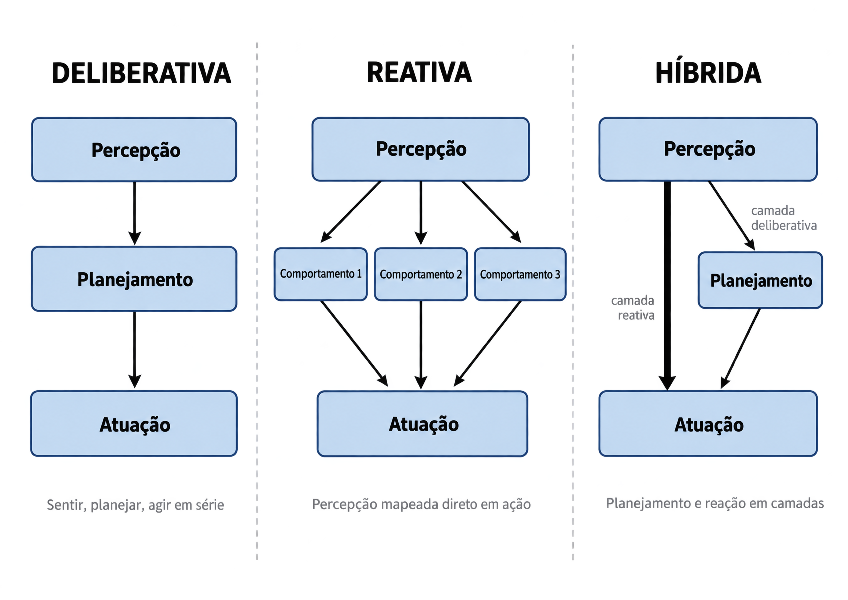
\includegraphics[width=0.8\textwidth]{figuras/fig_arquiteturas_roboticas.pdf}
    \caption{Paradigmas arquiteturais em robótica: as três colunas empregam as mesmas
    caixas --- percepção, planejamento e atuação ---, variando apenas como se conectam.
%% Corrigido em 14/11/2026: a legenda dizia que a camada reativa "alcanca a
%% atuacao sem passar pelo planejamento" e que esse e o paradigma da proposta. Nao e o
%% da implementacao: a camada reativa envia METAS ao Nav2, que continua planejando e
%% controlando, e permanece o unico produtor de /cmd_vel. O que a reacao contorna e a
%% DECISAO da patrulha sobre para onde ir, nao o planejamento do movimento.
    A via rápida em traço grosso na coluna híbrida é a camada reativa, que no esquema
    canônico alcança a atuação sem passar pelo planejamento. A arquitetura proposta no
    Capítulo~\ref{cap:proposta} segue esse paradigma em um sentido mais restrito, que
    convém fixar desde já: a camada reativa \emph{preempta a decisão} da patrulha sobre
    qual meta perseguir, mas não contorna o planejamento nem o controle de movimento ---
    ela envia metas ao Nav2, que permanece o único produtor de comandos de velocidade.}
    \legend{Fonte: Adaptado de \citeonline{Kortenkamp2016} e
    \citeonline{Brugali2009ComponentI}.}
    \label{fig:arquiteturas_roboticas}
\end{figure}


\subsection{Introdução ao ROS e ROS2}

O Robot Operating System (ROS) surgiu como uma resposta aos desafios arquiteturais dos sistemas robóticos, oferecendo um framework flexível e ferramentas para o desenvolvimento de software robótico \cite{Quigley2009}.

\subsubsection{Visão Geral do ROS}

Contrariamente ao que o nome sugere, o ROS não é um sistema operacional no sentido tradicional, mas sim um middleware que fornece serviços de comunicação, abstração de hardware, gerenciamento de pacotes e ferramentas para desenvolvimento de aplicações robóticas \cite{Quigley2009, Joseph2018}.

Os principais objetivos do ROS incluem abstração de hardware, computação distribuída, reutilização de código, ferramentas para testes e depuração, e criação de um ecossistema de software para a comunidade robótica \cite{Quigley2009}.

\subsubsection{Evolução para ROS2}

Apesar do sucesso do ROS, limitações em seu design original levaram ao desenvolvimento do ROS2, uma reimplementação completa que visa abordar essas limitações e adaptar-se às novas tendências em robótica \cite{Macenski2022}.

As motivações declaradas para o desenvolvimento do ROS2
\cite{Macenski2022, ROS2Design2024} dividem-se entre garantias que o ROS original não
dava e contextos que ele não atendia. Do primeiro grupo são o suporte a tempo real, os
mecanismos de segurança de autenticação, autorização e criptografia, a robustez em redes
não ideais e a confiabilidade exigida por aplicação industrial. Do segundo, a otimização
para sistemas embarcados de recurso limitado e o suporte nativo à coordenação de
múltiplos robôs. A primeira dessas garantias é a que importa ao Capítulo~\ref{cap:proposta},
e a Seção~\ref{sec:prop-relogios} mostra que tê-la disponível não equivale a tê-la
usada corretamente.

\subsection{Arquitetura e Componentes do ROS/ROS2}

Tanto o ROS quanto o ROS2 seguem uma arquitetura baseada em componentes, com alguns conceitos fundamentais compartilhados, embora com implementações diferentes \cite{Quigley2009, Macenski2022}.

\subsubsection{Conceitos Fundamentais}

\paragraph{Nós}

Os nós são os processos computacionais básicos no ROS/ROS2, responsáveis por realizar computações específicas \cite{Quigley2009, Joseph2018}. Em ROS, os nós são processos independentes que se comunicam através do ROS Master. Em ROS2, os nós podem ser processos independentes ou componentes dentro de um mesmo processo, com comunicação gerenciada pelo middleware DDS \cite{Macenski2022}.

\paragraph{Tópicos}

Os tópicos são canais de comunicação unidirecional que seguem o padrão publicador/assinante \cite{Quigley2009, Joseph2018}. Um nó publica mensagens em um tópico, e qualquer nó interessado pode se inscrever para receber essas mensagens. A comunicação via tópicos é assíncrona e desacoplada, adequada para transmissão contínua de dados como leituras de sensores ou estados do robô \cite{Macenski2022}.

\paragraph{Serviços e Ações}

Os serviços seguem o padrão cliente/servidor, onde um nó faz uma solicitação a outro e espera por uma resposta \cite{Quigley2009, Joseph2018}. São síncronos e adequados para operações discretas que requerem uma resposta.

As ações são uma extensão dos serviços para operações de longa duração, consistindo em uma meta, feedback durante a execução e um resultado final \cite{Joseph2018, Macenski2022}. São adequadas para tarefas como navegação ou manipulação de objetos.

\paragraph{Parâmetros e Bags}

Os parâmetros são valores de configuração que podem ser acessados e modificados pelos nós \cite{Quigley2009, Joseph2018}. Em ROS, são gerenciados pelo Parameter Server; em ROS2, pelos próprios nós.

Os bags são um formato de arquivo para armazenar e reproduzir mensagens ROS/ROS2, úteis para gravar dados durante a execução e reproduzi-los posteriormente para análise ou teste \cite{Quigley2009, Joseph2018}.

\subsubsection{Middleware e Comunicação}

Uma das principais diferenças entre ROS e ROS2 está na camada de middleware que gerencia a comunicação entre os componentes do sistema \cite{Macenski2022, ROS2Design2024}. A \autoref{fig:ros_vs_ros2} contrasta as duas arquiteturas de descoberta, separando o que é registro do que é tráfego de dados.

\paragraph{ROS Master vs. DDS}
\begin{figure}[h]
    \centering
%% Figura refeita em 14/11/2026. Na versao anterior o "Middleware DDS" aparecia como
%% hub central do painel ROS2, na mesma posicao e topologia do ROS Master a esquerda --
%% de modo que os dois paineis mostravam a MESMA arquitetura com nomes diferentes no
%% meio, apagando justamente a diferenca que a secao descreve. No painel ROS, todas as
%% ligacoes passavam pelo Master, reproduzindo o equivoco de que os dados trafegam por
%% ele. A fonte tambem nao citava nada ("documentacao oficial", sem referencia).
    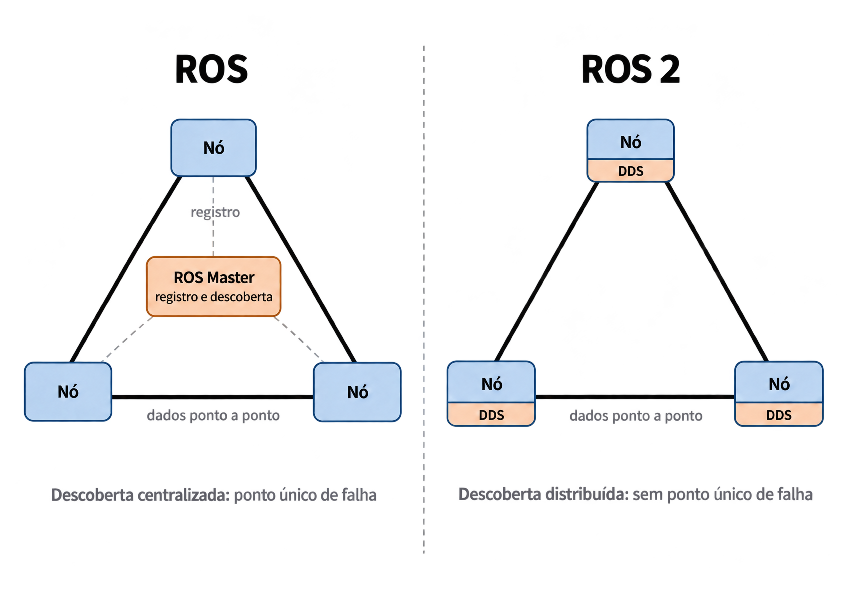
\includegraphics[width=0.8\textwidth]{figuras/fig_ros_vs_ros2.pdf}
    \caption{Arquiteturas de descoberta no ROS e no ROS~2, com os nós nas mesmas
    posições nos dois painéis. À esquerda, o registro (tracejado) é centralizado no ROS
    Master, enquanto os dados (linha cheia) trafegam ponto a ponto. À direita não há
    elemento central: o DDS reside dentro de cada nó e a descoberta é distribuída.}
    \legend{Fonte: Elaborada pelo autor com base em \citeonline{Macenski2022} e na
    documentação de projeto do ROS~2 \cite{ROS2Design2024}.}
    \label{fig:ros_vs_ros2}
\end{figure}

%% Precisado em 14/11/2026, junto com a figura: dizer que "a comunicacao e gerenciada
%% pelo ROS Master" induz a ideia de que os dados trafegam por ele, o que a figura nova
%% desmente explicitamente ao separar registro (tracejado) de dados (linha cheia).
No ROS original, é a \emph{descoberta} entre nós que é gerenciada pelo ROS Master, um serviço centralizado que mantém o registro de todos os nós, tópicos e serviços ativos \cite{Quigley2009, Joseph2018}. Concluída a negociação, os nós trocam mensagens diretamente entre si, ponto a ponto, sem que os dados passem pelo Master. Esta centralização da descoberta simplifica a implementação, mas introduz um ponto único de falha: sem o Master, nenhum nó novo encontra os demais.

O ROS2 substitui o ROS Master por uma arquitetura baseada em DDS (Data Distribution Service), um padrão aberto para comunicação publicador/assinante em sistemas distribuídos \cite{Macenski2022, ROS2Design2024}. O DDS oferece recursos avançados como descoberta distribuída, qualidade de serviço (QoS), segurança, persistência e filtragem de conteúdo.

\paragraph{Modelo de Computação}

No ROS original, cada nó é tipicamente um processo independente \cite{Quigley2009, Joseph2018}. O ROS2 introduz o conceito de composição de nós, permitindo que múltiplos nós sejam executados dentro do mesmo processo \cite{Macenski2022, ROS2Design2024}, reduzindo a sobrecarga de comunicação e permitindo compartilhamento mais eficiente de recursos.

Os executores em ROS2 gerenciam a execução de callbacks associados a tópicos, serviços, ações e timers, com diferentes tipos disponíveis (SingleThreadedExecutor, MultiThreadedExecutor, StaticSingleThreadedExecutor) para diferentes necessidades \cite{Macenski2022, ROS2Design2024}.

\subsection{Simulação e Validação}

A simulação é essencial no desenvolvimento de sistemas robóticos, permitindo testar algoritmos em ambientes virtuais antes da implementação em hardware real \cite{Siegwart2011}.

\subsubsection{Simuladores Integrados}

O ROS/ROS2 integra-se com diversos simuladores \cite{Joseph2018, Macenski2022}. O
\textbf{Gazebo} foi desenvolvido especificamente para robótica e oferece simulação de
física, de sensores, ambientes personalizáveis e extensibilidade por \textit{plugins}; é
o usado nesta tese. Webots, CoppeliaSim (V-REP), CARLA, voltado a veículos autônomos, e
Isaac Sim, da NVIDIA, também se integram ao ROS/ROS2.

\subsubsection{Ferramentas de Simulação e Teste}

O ROS/ROS2 oferece ferramentas como URDF/XACRO para descrição de robôs, RViz para visualização 3D, e rqt para interfaces gráficas \cite{Joseph2018, Macenski2022}. Para validação, integra-se com frameworks de teste unitário (GTest, pytest) e oferece ferramentas para testes de integração e integração contínua \cite{Joseph2018, Macenski2022}.

%% Subsecao NOVA em 15/11/2026, construida em torno do paragrafo que antes era a cauda
%% orfa de "Tendencias e Desenvolvimentos Futuros". O determinismo de temporizacao e a
%% unica materia desta secao que reaparece nos capitulos posteriores (15 ocorrencias de
%% tempo simulado / relogio de parede neles, contra 2 aqui), e e a fundamentacao do
%% defeito relatado na Secao 6.13. Merecia subsecao, nao um paragrafo pendurado no fim.
%% Removidas no mesmo passo as subsecoes de Integracao de Sensores e Atuadores,
%% Desenvolvimento de Aplicacoes, Aplicacoes e Casos de Uso e Tendencias: zero
%% ocorrencias de catkin, ament_cmake, setuptools, rosbag, rostopic, rosparam, tf,
%% manipulador, micro-ROS e computacao em nuvem em QUALQUER outro capitulo da tese.
\subsection{Tempo Simulado e Determinismo de Temporização}
\label{sec:fund-relogios}

Em simulação, o \ac{ROS}~2 permite que todos os nós compartilhem uma base de tempo
publicada pelo simulador, em vez do relógio do sistema operacional. Habilitado o
parâmetro correspondente, os temporizadores de cada nó passam a ser disparados por esse
tempo \emph{simulado}, de sorte que uma pausa do simulador pausa também o agendamento, e
uma simulação que corra mais devagar ou mais depressa que o tempo real não altera o
intervalo \emph{percebido} entre dois disparos \cite{Macenski2022}. É essa propriedade que
torna um experimento em simulação repetível, independentemente da carga da máquina em que
roda.

A propriedade, porém, vale para o mecanismo de agendamento, não para o código agendado.
Um temporizador pode ser disparado em tempo simulado enquanto a função que ele chama
consulta, internamente, o relógio de parede do processo --- e nada na interface sinaliza a
divergência, porque as duas leituras têm o mesmo tipo e a mesma aparência. Se essa função
compara dois instantes para decidir se um intervalo transcorreu, ela passa a medir numa
base de tempo e a ser chamada em outra, e o intervalo efetivo deixa de ser o
especificado. A Seção~\ref{sec:prop-relogios} descreve a ocorrência desse padrão na
implementação avaliada neste trabalho, e a Seção~\ref{sec:res-verificacao-relogio} mede a sua
consequência sobre os desfechos.
\section{Navegação Reativa em Robótica Móvel}

A navegação é uma capacidade fundamental para robôs móveis autônomos, permitindo que se desloquem de forma segura e eficiente em ambientes diversos. Esta seção apresenta os principais paradigmas de navegação robótica, com ênfase na navegação reativa, particularmente relevante para aplicações em ambientes dinâmicos e não estruturados como subestações elétricas.

\subsection{Paradigmas de Navegação Robótica}
A \autoref{fig:paradigmas_navegacao} mostra como a navegação robótica pode ser classificada em diferentes paradigmas, cada um com abordagens distintas para o problema de deslocamento autônomo \cite{Siegwart2011, Murphy2000}.

\begin{figure}[h]
    \centering
%% Figura refeita em 14/11/2026. A versao anterior estava errada e era redundante: a
%% coluna "Hibrida" trazia TRES caixas "Act" e NENHUMA "Plan", apagando o planejamento
%% justo onde ele define o conceito; os rotulos estavam em ingles; e o desenho repetia
%% a tricotomia da Figura~\ref{fig:arquiteturas_roboticas}, a uma secao de distancia.
%% A versao atual mostra o que e especifico de NAVEGACAO -- a mesma planta com os
%% mesmos obstaculos, variando o tracado --, de modo que as duas figuras deixam de se
%% sobrepor.
    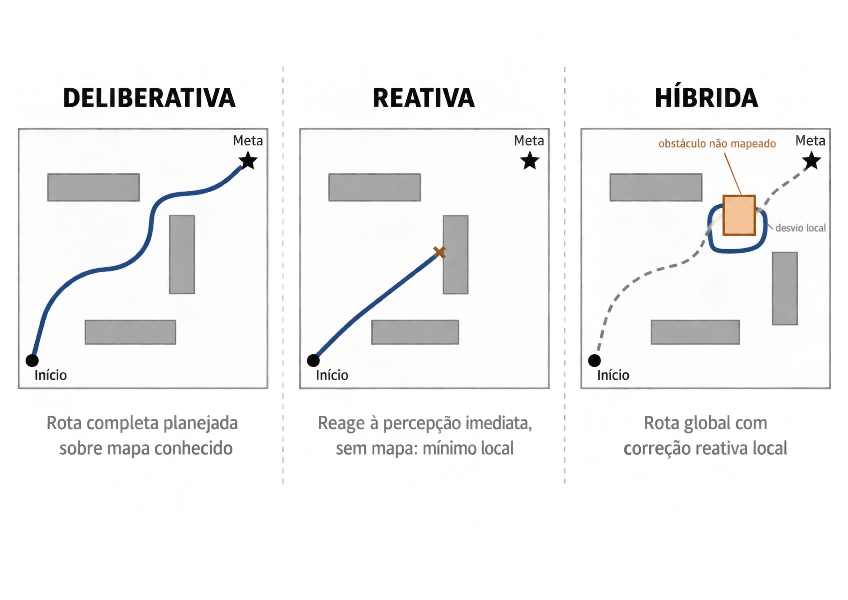
\includegraphics[width=0.8\textwidth]{figuras/fig_paradigmas_navegacao.pdf}
    \caption{Paradigmas de navegação robótica sobre a mesma planta: à esquerda, a rota
    completa planejada sobre mapa conhecido; ao centro, a reação à percepção imediata,
    que sem mapa fica retida num mínimo local antes de alcançar a meta; à direita, a
    rota global corrigida localmente ao encontrar um obstáculo não mapeado.}
    \legend{Fonte: Adaptado de \citeonline{Siegwart2011} e \citeonline{Murphy2000}.}
    \label{fig:paradigmas_navegacao}
\end{figure}


\subsubsection{Navegação Deliberativa}

A navegação deliberativa segue o paradigma Sense-Plan-Act (SPA), onde o robô percebe o ambiente, constrói um modelo interno, planeja uma trajetória completa e então a executa \cite{Murphy2000}. Suas principais características incluem:

\begin{itemize}
    \item Representação explícita do ambiente através de mapas detalhados
    \item Planejamento global de trajetórias completas
    \item Busca por soluções ótimas segundo critérios específicos
    \item Maior complexidade computacional
    \item Sensibilidade a incertezas e discrepâncias no modelo do ambiente
\end{itemize}

\subsubsection{Navegação Reativa}

Em contraste, a navegação reativa baseia-se no paradigma Sense-Act, eliminando a fase explícita de planejamento \cite{Brooks1986, Arkin1998}. O robô reage diretamente aos estímulos sensoriais, sem construir um modelo completo do ambiente. Suas características incluem:

\begin{itemize}
    \item Ausência de representação explícita do ambiente
    \item Decisões baseadas apenas na percepção imediata
    \item Baixa complexidade computacional
    \item Robustez a incertezas e mudanças no ambiente
    \item Possibilidade de soluções subótimas ou mínimos locais
\end{itemize}

\subsubsection{Navegação Híbrida}

A navegação híbrida combina elementos das abordagens deliberativa e reativa \cite{Murphy2000, Arkin1998}, tipicamente organizados em camadas:

\begin{itemize}
    \item Camada deliberativa para planejamento global e raciocínio de alto nível
    \item Camada reativa para respostas rápidas a eventos imprevistos
    \item Camada intermediária para coordenação entre as demais
\end{itemize}

Exemplos incluem a arquitetura 3T \cite{Bonasso1997}, AuRA \cite{Arkin1987} e Saphira \cite{Konolige1997}.

\subsection{Navegação Baseada em Comportamentos}

A navegação baseada em comportamentos é uma abordagem reativa que organiza o controle do robô em módulos comportamentais simples e independentes \cite{Arkin1998, Brooks1986}.

\subsubsection{Arquitetura de Subsunção}

A Arquitetura de Subsunção, proposta por Rodney Brooks \cite{Brooks1986}, organiza os comportamentos em camadas hierárquicas, onde comportamentos de nível superior podem suprimir ou inibir comportamentos de nível inferior. Suas características incluem:

\begin{itemize}
    \item Decomposição vertical em níveis de competência
    \item Incrementalidade na construção do sistema
    \item Mecanismos de supressão e inibição para coordenação
    \item Ausência de representação central do ambiente
\end{itemize}

Uma implementação típica inclui comportamentos como evitar obstáculos (nível básico), vagar, explorar, construir mapas e identificar objetos (níveis superiores) \cite{Brooks1986}.

\subsubsection{Esquemas Motores}

A abordagem de Esquemas Motores, proposta por Ronald Arkin \cite{Arkin1989}, utiliza fusão de comportamentos através de soma vetorial. Suas características incluem:

\begin{itemize}
    \item Representação vetorial de cada comportamento
    \item Fusão por soma ponderada dos vetores
    \item Pesos adaptativos para os comportamentos
    \item Paralelismo na contribuição dos comportamentos
\end{itemize}

A equação básica para a fusão de comportamentos é:

\begin{equation}
\vec{v} = \sum_{i=1}^{n} w_i \cdot \vec{v_i}
\end{equation}

onde $\vec{v}$ é o vetor resultante, $\vec{v_i}$ é o vetor gerado pelo comportamento $i$, $w_i$ é o peso associado ao comportamento $i$, e $n$ é o número total de comportamentos \cite{Arkin1998}.

\subsection{Campos Potenciais e Navegação Reativa}

O método de Campos Potenciais, introduzido por Oussama Khatib \cite{Khatib1986}, representa o ambiente como um campo de forças, onde o robô é atraído pelo objetivo e repelido por obstáculos.

\subsubsection{Princípios Fundamentais}

No método de Campos Potenciais, o robô é tratado como uma partícula sob influência de um campo potencial artificial $U(q)$, que é a soma de um potencial atrativo $U_{att}(q)$ gerado pelo objetivo e potenciais repulsivos $U_{rep}(q)$ gerados pelos obstáculos \cite{Khatib1986, Siegwart2011}:

\begin{equation}
U(q) = U_{att}(q) + U_{rep}(q)
\end{equation}

A força resultante que atua sobre o robô é o gradiente negativo do potencial total:

\begin{equation}
F(q) = -\nabla U(q) = -\nabla U_{att}(q) - \nabla U_{rep}(q) = F_{att}(q) + F_{rep}(q)
\end{equation}

O potencial atrativo é tipicamente definido como uma função quadrática da distância ao objetivo:

\begin{equation}
U_{att}(q) = \frac{1}{2} \xi \|q - q_{goal}\|^2
\end{equation}

O potencial repulsivo cresce à medida que o robô se aproxima de obstáculos:

\begin{equation}
U_{rep}(q) = 
\begin{cases}
\frac{1}{2} \eta \left(\frac{1}{\rho(q)} - \frac{1}{\rho_0}\right)^2, & \text{se } \rho(q) \leq \rho_0 \\
0, & \text{se } \rho(q) > \rho_0
\end{cases}
\end{equation}

onde $\eta$ é um fator de escala, $\rho(q)$ é a distância ao obstáculo mais próximo e $\rho_0$ é a distância de influência do obstáculo \cite{Khatib1986, Siegwart2011}.

\subsubsection{Limitações e Extensões}

Apesar de sua simplicidade e eficiência computacional, o método de Campos Potenciais apresenta algumas limitações \cite{Koren1991, Siegwart2011}:

\begin{itemize}
    \item Mínimos locais que podem "aprisionar" o robô
    \item Oscilações em passagens estreitas
    \item Dificuldades quando o objetivo está próximo a obstáculos
    \item Falta de consideração da dinâmica do robô
\end{itemize}

Diversas extensões foram propostas para superar estas limitações, incluindo Campos Potenciais Harmônicos \cite{Connolly1990}, combinação com navegação em grafo \cite{Barraquand1992}, e abordagens evolutivas \cite{Vadakkepat2000}.

\subsubsection{Aplicações em Robótica Móvel}

O método de Campos Potenciais tem sido aplicado com sucesso em diversas áreas \cite{Siegwart2011, Arkin1998}:

\begin{itemize}
    \item Robôs móveis terrestres para navegação em ambientes internos e externos
    \item Veículos aéreos não tripulados para navegação 3D
    \item Robôs manipuladores para planejamento de movimento
    \item Sistemas multi-robôs para coordenação de enxames
\end{itemize}

Em aplicações de inspeção de subestações elétricas, a navegação reativa baseada em campos potenciais oferece vantagens significativas devido à sua capacidade de responder rapidamente a obstáculos imprevistos e adaptar-se a ambientes dinâmicos \cite{Lactec2022, Iberdrola2022}.

\subsection{SLAM (Simultaneous Localization and Mapping)}

O SLAM é um problema fundamental em robótica móvel que consiste em construir um mapa do ambiente desconhecido enquanto simultaneamente se localiza neste mapa \cite{Durrant2006, Thrun2005}.

\subsubsection{O Problema do SLAM}
Os principais desafios do SLAM incluem incertezas na odometria e nas medições, associação de dados, alta dimensionalidade do espaço de estados e ambiguidade perceptual \cite{Durrant2006, Thrun2005}. A \autoref{fig:problema_slam} mostra uma visão geral do uso do SLAM na navegação.

\begin{figure}[h]
    \centering
%% Figura refeita em 14/11/2026. A versao anterior nao mostrava o problema: exibia
%% quatro setas soltas entre robo, ambiente e mapa, sem a circularidade que e a
%% dificuldade inteira do SLAM. Equiparava ainda "comandos de controle" e "odometria"
%% num unico rotulo, sendo que u sao os comandos e a odometria e a medida do
%% deslocamento resultante, com incerteza propria.
    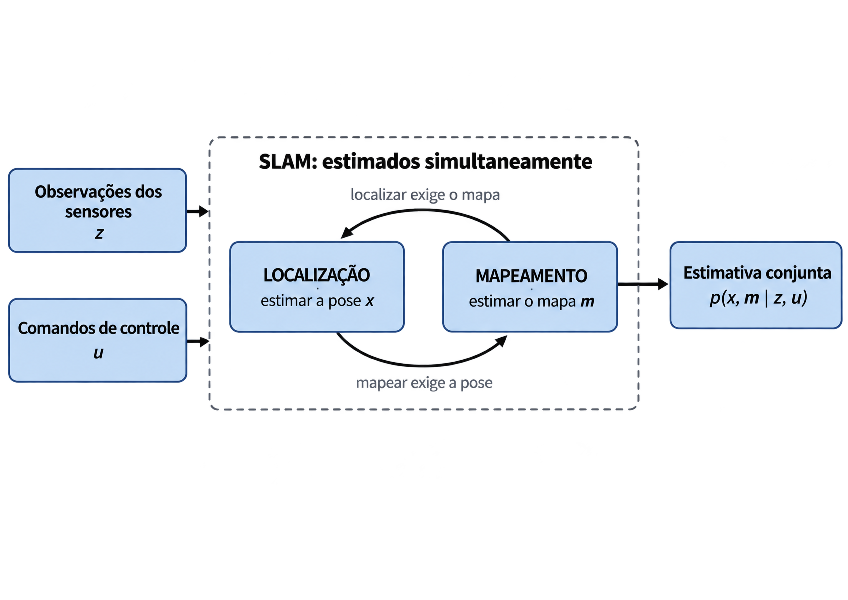
\includegraphics[width=0.8\textwidth]{figuras/fig_problema_slam.pdf}
    \caption{O problema do SLAM: localizar exige o mapa e mapear exige a pose, de modo
    que as duas estimativas são mutuamente dependentes e precisam ser resolvidas
    simultaneamente, a partir das observações $z$ e dos comandos de controle $u$.}
    \legend{Fonte: Adaptado de \citeonline{Durrant2006} e \citeonline{Thrun2005}.}
    \label{fig:problema_slam}
\end{figure}

O problema do SLAM pode ser formulado probabilisticamente como a estimação da distribuição de probabilidade conjunta \cite{Durrant2006, Thrun2005}:

\begin{equation}
p(x_{1:t}, m | z_{1:t}, u_{1:t}, x_0)
\end{equation}

onde $x_{1:t}$ são os estados do robô, $m$ é o mapa do ambiente, $z_{1:t}$ são as observações sensoriais, $u_{1:t}$ são os comandos de controle, e $x_0$ é o estado inicial.


\subsubsection{Principais Abordagens}

Diversas abordagens foram desenvolvidas para resolver o problema do SLAM \cite{Durrant2006, Thrun2005, Cadena2016}:

\begin{itemize}
    \item \textbf{SLAM Baseado em Filtros}: Utiliza técnicas como EKF-SLAM (Extended Kalman Filter) \cite{Smith1990}, UKF-SLAM (Unscented Kalman Filter) \cite{Julier2004} e FastSLAM (filtros de partículas) \cite{Montemerlo2002}.
    
    \item \textbf{SLAM Baseado em Otimização}: Formula o problema como minimização de erro, incluindo Graph-SLAM \cite{Grisetti2010} e Pose Graph Optimization.
    
    \item \textbf{SLAM Visual}: Utiliza câmeras como principal sensor, incluindo MonoSLAM \cite{Davison2007}, Stereo SLAM \cite{Paz2008} e Visual-Inertial SLAM \cite{Mourikis2007}.
    
    \item \textbf{SLAM Baseado em LiDAR}: Utiliza sensores laser, incluindo Hector SLAM \cite{Kohlbrecher2011}, Cartographer \cite{Hess2016} e LOAM \cite{Zhang2014}.
\end{itemize}

\subsubsection{Representações de Mapas}

Diferentes representações de mapas são utilizadas em SLAM \cite{Thrun2005, Cadena2016}:

\begin{itemize}
    \item Mapas de Ocupação em Grade (discretização do espaço em células) \cite{Elfes1989}
    \item Mapas de Características (pontos, linhas ou cantos distintos) \cite{Smith1990}
    \item Mapas Topológicos (grafo de locais e conexões) \cite{Kuipers1991}
    \item Mapas Semânticos (com informações sobre objetos e regiões) \cite{Kostavelis2015}
    \item Mapas 3D (nuvens de pontos, malhas ou octrees) \cite{Hornung2013}
\end{itemize}

O fechamento de loop (reconhecer quando o robô retorna a um local visitado) é o que corrige a deriva acumulada na odometria: detectado o reencontro, mapa e trajetória estimada são reajustados \cite{Durrant2006, Cadena2016}.

\subsection{Integração de Modelos 3D em Navegação}

A integração de modelos 3D em sistemas de navegação robótica representa uma tendência importante, especialmente para aplicações em ambientes complexos como subestações elétricas \cite{Hornung2013, Rusu2011}.

\subsubsection{Representações 3D para Navegação}

Diversas representações 3D são utilizadas para navegação robótica \cite{Hornung2013, Rusu2011}:

\begin{itemize}
    \item \textbf{Nuvens de Pontos}: Conjuntos de pontos 3D obtidos de sensores como LiDAR ou câmeras de profundidade.
    
    \item \textbf{Octrees}: Estruturas hierárquicas que dividem o espaço 3D recursivamente, como o OctoMap \cite{Hornung2013}.
    
    \item \textbf{Malhas Poligonais}: Representações de superfícies através de polígonos conectados.
    
    \item \textbf{Mapas de Elevação}: Representações 2.5D que armazenam a altura do terreno para cada posição (x,y).
\end{itemize}

\subsubsection{Aquisição e Processamento de Dados 3D}

A aquisição de dados 3D para navegação pode ser realizada através de \cite{Rusu2011, Hornung2013}:

\begin{itemize}
    \item Sensores LiDAR 3D ou 2D com movimento
    \item Câmeras RGB-D (como Kinect ou RealSense)
    \item Sistemas de visão estéreo
    \item Fotogrametria e Structure from Motion
\end{itemize}

O processamento destes dados envolve técnicas como registro de nuvens de pontos, filtragem, segmentação, detecção de características e reconstrução de superfícies \cite{Rusu2011}.

\subsubsection{Aplicações em Subestações Elétricas}

A integração de modelos 3D em navegação robótica para inspeção de subestações elétricas oferece diversas vantagens \cite{Lactec2022, Iberdrola2022}:

\begin{itemize}
    \item \textbf{Planejamento de Trajetória 3D}: Permite considerar a estrutura vertical das subestações, incluindo equipamentos elevados e obstáculos em diferentes alturas.
    
    \item \textbf{Localização Precisa}: Melhora a precisão da localização do robô através da correspondência com modelos 3D detalhados.
    
    \item \textbf{Detecção de Mudanças}: Permite identificar alterações na estrutura da subestação através da comparação com modelos de referência.
    
    \item \textbf{Inspeção Baseada em Modelos}: Facilita a inspeção direcionada de componentes específicos, utilizando o modelo 3D como referência.
    
    \item \textbf{Visualização e Análise}: Melhora a visualização e análise dos dados de inspeção no contexto do modelo 3D da subestação.
\end{itemize}

\subsection{Desafios e Tendências}

A navegação reativa em robótica móvel, especialmente para aplicações em subestações elétricas, enfrenta diversos desafios e apresenta tendências emergentes \cite{Cadena2016, Lactec2022, Iberdrola2022}.

\subsubsection{Desafios Atuais}

\begin{itemize}
    \item \textbf{Robustez a Interferência Eletromagnética}: Garantir o funcionamento adequado dos sensores e algoritmos de navegação em ambientes com forte interferência eletromagnética.
    
    \item \textbf{Navegação em Ambientes Complexos}: Lidar com a complexidade estrutural das subestações, incluindo equipamentos de diferentes formas e tamanhos, cabos, estruturas elevadas, etc.
    
    \item \textbf{Adaptação a Condições Variáveis}: Adaptar-se a mudanças nas condições ambientais, como iluminação, clima e configuração da subestação.
    
    \item \textbf{Segurança}: Garantir a navegação segura em ambientes de alta tensão, evitando colisões com equipamentos críticos e mantendo distâncias de segurança.
\end{itemize}

\subsubsection{Tendências Emergentes}

\begin{itemize}
    \item \textbf{Navegação Semântica}: Incorporação de informações semânticas no processo de navegação, permitindo decisões baseadas no significado e função dos objetos no ambiente.
    
    \item \textbf{Aprendizado de Navegação}: Utilização de técnicas de aprendizado de máquina para melhorar o desempenho da navegação através da experiência.
    
    \item \textbf{Navegação Colaborativa}: Coordenação entre múltiplos robôs para inspeção e navegação mais eficientes.
    
    \item \textbf{Integração com Digital Twins}: Utilização de modelos digitais detalhados das subestações para melhorar o planejamento e execução da navegação.
\end{itemize}

A navegação reativa em robótica móvel, especialmente quando integrada com técnicas de SLAM e modelos 3D, oferece uma base sólida para o desenvolvimento de sistemas robóticos autônomos capazes de realizar inspeções eficientes e seguras em subestações elétricas, contribuindo para a manutenção preventiva e a confiabilidade do sistema elétrico.



% ----------------------------------------------------------
% Revisão Crítica da Literatura
% ----------------------------------------------------------
%% Revisao estilistica em 15/11/2026, 34 trechos. Este capitulo concentrava as
%% formulas repetidas do documento, contadas antes da passagem:
%%   3x "Apesar dos avancos significativos, [...] ainda enfrenta desafios
%%      importantes" -- abertura IDENTICA das analises criticas de 3.1.5,
%%      3.2.5 e 3.3.5;
%%   3x "O periodo 2015-2025 testemunhou" -- abertura de 3.2.1, 3.3.1 e 3.4.1;
%%   3x "A integracao efetiva de conhecimento de dominio especifico";
%%   4x "representa um desafio significativo"; 3x "permanece problematica";
%%   2x "Um avanco particularmente relevante"; 2x "Mais recentemente,
%%      arquiteturas baseadas em Transformers"; 23x "significativ*".
%% Cada abertura passou a entrar pelo gargalo tecnico do proprio eixo (custo
%% embarcado, desalinhamento de resolucao e taxa, acoplamento mapa-controle), e
%% cada fechamento, antes uma "direcao promissora para pesquisas futuras",
%% passou a declarar a posicao desta tese em relacao aquele gargalo -- inclusive
%% quando a posicao e nao atacar o problema. Nenhuma referencia foi trocada,
%% acrescentada ou removida nesta passagem; confira com
%%   git diff -U0 -- cap_revisao_bib/revisao.tex | grep -c '\\cite'
%% Renomeado em 13/11/2026. O capitulo nao executa protocolo de revisao sistematica
%% -- nao ha bases, consultas, datas, criterios de inclusao, numero de registros nem
%% processo de selecao documentados -- e chamar-se sistematico prometia um metodo que
%% nao foi realizado. Passa a declarar o que de fato e: revisao critica, com o critério
%% de selecao explicitado abaixo e com o alcance da selecao reconhecido.
%% Titulo alterado em 15/11/2026. Era "Revisao Critica da Literatura" -- o unico
%% titulo da tese que afirmava uma QUALIDADE em vez de nomear o conteudo, ao lado de
%% "Fundamentacao Teorica", "Avaliacao Experimental", "Resultados e Discussao" e
%% "Conclusao". Criticidade e coisa que o leitor julga. As quatro subsecoes chamadas
%% "Analise Critica e Desafios Futuros" passaram a nomear o que de fato discutem.
\chapter{Revisão da Literatura}
\label{cap:revisao}

A inspeção de subestações elétricas é tarefa predominantemente humana em ambiente energizado, e é desse fato que decorre o interesse por automatizá-la: há limite de segurança para a aproximação a equipamento sob tensão, os eventos de interesse são esparsos ao longo de rotas fixadas por norma, e o custo por inspeção é alto. Os \ac{VTA}, também chamados \ac{RMT} ou \ac{UGV}, são a plataforma em que essa automação tem sido tentada, e a navegação autônoma é a função de que as demais dependem.

Esta revisão analisa criticamente o estado da arte na integração de Aprendizado por Reforço, Visão Computacional e Fusão de Sensores para navegação autônoma de \ac{UGV} em ambientes industriais desafiadores, com ênfase no contexto de subestações elétricas, no período entre 2015 e 2025.

É uma \emph{revisão crítica}, e não uma revisão sistemática: não se executou protocolo prospectivo com bases, consultas, datas de busca, critérios de inclusão e exclusão, número de registros recuperados e processo de seleção documentado. A seleção foi feita por amostragem orientada ao problema: trabalhos recuperados em busca temática nas três áreas e, dentro delas, os que (i) tratam navegação ou inspeção robótica autônoma, (ii) são citáveis por identificador verificável e (iii) sustentam ou contradizem alguma afirmação feita nesta tese. O alcance dessa seleção é, portanto, limitado: ela não autoriza alegação de cobertura exaustiva da literatura, e as lacunas apontadas adiante devem ser lidas como lacunas \emph{nesta amostra}, não como ausências demonstradas no campo.

Os trabalhos citados ao longo do capítulo foram conferidos individualmente por identificador (DOI ou endereço resolvível) quanto a autoria, título, veículo e ano, e as afirmações atribuídas a cada um foram confrontadas com o conteúdo do trabalho.

\section{Aprendizado por Reforço (RL) e Aprendizado por Reforço Profundo (DRL)}

Enquanto o Capítulo 2 apresentou os fundamentos teóricos do Aprendizado por Reforço, esta seção analisa criticamente sua evolução e aplicações específicas em navegação autônoma de \ac{UGV} no período 2015-2025, com foco em ambientes industriais complexos como subestações elétricas.

\subsection{Evolução dos Algoritmos DRL para Navegação Robótica}

A trajetória dos algoritmos de \ac{DRL} para navegação robótica responde a uma limitação precisa dos métodos clássicos, a de exigir um modelo do ambiente que o robô raramente possui. %% Corrigido em 14/11/2026 (auditoria bibliografica, duas correcoes nesta frase):
%% (i) Tai2017 era descrito como uso de DQN. O trabalho e de CONTROLE CONTINUO,
%% treinado por DDPG assincrono -- DQN opera sobre acoes discretas e nao e o
%% algoritmo da fonte; (ii) dizia-se que Zhu2017 "expandiu" Tai2017, e mais adiante
%% nesta mesma revisao dizia-se o inverso. Os dois trabalhos sao de 2017 e
%% independentes; a genealogia nao e demonstravel e foi substituida por comparacao
%% factual entre as abordagens.
\citeonline{Tai2017} demonstraram navegação sem mapa de robôs móveis por aprendizado
profundo com \emph{controle contínuo}, treinada por \ac{DDPG} assíncrono e alimentada
diretamente por leituras esparsas de laser, com transferência da política do simulador
para o robô real. \citeonline{Zhu2017}, no mesmo ano e por via independente, trataram
a navegação dirigida a alvo a partir de imagens, dispensando igualmente mapa explícito,
mas tomando como entrada a cena visual e o alvo desejado em vez de distâncias.

\citeonline{Schulman2017} propuseram o \ac{PPO}, que se tornou padrão na área pela estabilidade do passo de atualização. \citeonline{Haarnoja2018} introduziram o \ac{SAC}, que incorpora um termo de entropia na função objetivo, resultando em políticas mais robustas e explorativas. Análises comparativas realizadas por \citeonline{Ibarz2021} demonstraram que algoritmos baseados em política como \ac{PPO} e \ac{SAC} geralmente superam métodos baseados em valor como \ac{DQN} em tarefas de navegação robótica com espaços de ação contínuos.

\subsection{Abordagens Sim-to-Real para Navegação Autônoma}

Política treinada apenas em simulação degrada-se no robô físico por efeito do \textit{reality gap}, a discrepância entre a dinâmica modelada no simulador e o comportamento dos sensores e atuadores em operação. \citeonline{Tobin2017} introduziram o \textit{Domain Randomization}, que varia deliberadamente os parâmetros da simulação durante o treinamento, tornando a política robusta o suficiente para operar no domínio real.

\citeonline{Peng2018} expandiram esta abordagem com o conceito de \textit{Dynamics Randomization}, focando especificamente na variabilidade dos parâmetros físicos. \citeonline{Sadeghi2017} demonstraram navegação visual sem necessidade de dados reais durante o treinamento, utilizando apenas ambientes simulados com randomização visual extensiva.
%% Frase removida em 13/11/2026 (auditoria bibliografica): atribuia a um trabalho
%% nao localizado em nenhuma base uma abordagem hibrida de randomizacao de dominio
%% com adaptacao adversarial.

Estudos comparativos realizados por \cite{Hwangbo2019} e \citeonline{Loquercio2021} demonstraram que abordagens Sim-to-Real bem projetadas podem atingir desempenho comparável ou superior a métodos treinados diretamente no mundo real, com fração do custo e tempo de desenvolvimento.

%% Ligacao acrescentada em 15/11/2026. Esta subsecao quase foi removida por nao ter
%% ocorrencia nos Capitulos 4 a 7 -- criterio que estava errado aqui: ela e o que
%% posiciona a limitacao de escopo mais importante da tese, declarada na Secao 7.3
%% ("a avaliacao e em simulacao"). O criterio certo nao e se o tema reaparece, e sim
%% se alguma afirmacao do trabalho depende dele.
Esta frente é a que situa o limite de escopo desta tese. A avaliação do
Capítulo~\ref{cap:avaliacao} é inteiramente simulada e nenhuma transferência para
\textit{hardware} foi tentada, de sorte que o que aqui se mede é a lógica de decisão da
arquitetura, e não o seu desempenho em pátio. A literatura acima descreve o que separa
uma coisa da outra, e é contra ela que a Seção~\ref{sec:conc-escopo} delimita o alcance
dos resultados.

\subsection{Aprendizado por Reforço Seguro para Ambientes Industriais}

A segurança é uma preocupação primordial na navegação autônoma em ambientes industriais como subestações elétricas. \citeonline{Garciaetal2015} levantaram os métodos de \ac{RL} Seguro e os organizaram em três famílias, conforme o que cada uma modifica: a função de recompensa, o processo de exploração ou o critério de otimização.

\citeonline{Achiam2017} introduziram o \ac{CPO}, um algoritmo que garante restrições de segurança durante o processo de otimização da política. \citeonline{Chow2018} expandiram esta abordagem com o conceito de \ac{CMDP}, onde o objetivo é maximizar a recompensa enquanto se satisfaz restrições de custo. %% Corrigido em 14/11/2026: a frase atribuia a Thananjeyan2021 funcoes de barreira e
%% garantia de invariancia em conjunto seguro, e situava o trabalho em navegacao
%% industrial. O titulo da propria entrada e "Recovery RL: safe reinforcement learning
%% with LEARNED recovery zones": o mecanismo e um critico de seguranca APRENDIDO que
%% alterna entre politica de tarefa e politica de recuperacao. Nada ali garante
%% invariancia, e os ensaios nao sao de navegacao industrial. Garantia formal nao se
%% atribui a uma fonte sem que a fonte a demonstre.
\citeonline{Thananjeyan2021} seguiram outro caminho: em vez de restringir a
otimização, aprenderam um crítico de segurança a partir de violações observadas e o
usaram para alternar entre uma política de tarefa e uma política de recuperação quando
o risco estimado cresce. A salvaguarda é, portanto, aprendida e probabilística: não
oferece a garantia de invariância que uma função de barreira persegue.

Para ambientes com requisito de segurança explícito, \citeonline{Brunke2022} combinam \ac{RL} com controladores de segurança baseados em modelo que podem intervir quando a política aprendida propõe ações potencialmente perigosas. Esta abordagem híbrida permite explorar os benefícios do aprendizado adaptativo enquanto mantém garantias formais de segurança.

%% Ligacao acrescentada em 15/11/2026, pela mesma razao da subsecao anterior: e o que
%% da sentido a frase da Secao 7.2 -- "esses sao os limites da evidencia de seguranca,
%% e nao uma garantia de seguranca".
A distinção entre essas vias importa ao que esta tese pode e não pode afirmar. A
precedência categórica de segurança do Capítulo~\ref{cap:proposta} é regra de projeto,
verificável por inspeção do código, e não garantia probabilística aprendida nem
invariância demonstrada por função de barreira. O que o
Capítulo~\ref{cap:resultados} apresenta é evidência empírica sobre o comportamento dessa
regra num conjunto de execuções, com os seus intervalos declarados --- e é precisamente
por existirem as garantias formais descritas acima que convém dizer que não se
reivindica nenhuma delas.

\subsection{Aplicações Específicas em Subestações Elétricas}

A aplicação de \ac{DRL} para navegação de \ac{UGV} em subestações elétricas apresenta desafios particulares devido à interferência eletromagnética, obstáculos metálicos e requisitos rigorosos de segurança. O ambiente eletromagnético da instalação é, por si, objeto de estudo e de indexação própria na literatura de compatibilidade eletromagnética de subestações \cite{He2007EMCSubstation}, e o estado da pesquisa e do desenvolvimento em robôs de inspeção para esse ambiente foi recentemente revisado por \citeonline{Wei2024Advancements}.

%% Reescrito em 13/11/2026 (auditoria bibliografica). A referencia anterior deste
%% paragrafo nao foi localizada no Crossref nem no OpenAlex; a segunda existe, mas
%% trata de fusao DGPS/dead reckoning para estimacao de pose, e nao de integracao
%% entre DRL e navegacao classica. As duas frases foram refeitas sobre o que os
%% trabalhos efetivamente publicados dizem.
\citeonline{Ou2024SensorFusionDRL} combinaram \ac{DRL} com fusão de sensores para navegação autônoma de robô móvel, ilustrando a frente em que a política de movimento é aprendida a partir de observações já fundidas. Em subestações, os sistemas descritos em operação seguem via distinta: \citeonline{Yan2024CombinedNav} relatam navegação combinada por fusão DGPS/\textit{dead reckoning} para robô de inspeção, na qual o objeto da fusão é a estimação de pose, e não a política de decisão.

Estudos de caso conduzidos por \cite{Lactec2022} e \cite{Iberdrola2022} em subestações reais demonstraram a viabilidade prática destas abordagens, e relatam ganho de eficiência e de cobertura de inspeção sobre os métodos tradicionais, sem decompor esse ganho por mecanismo.

\subsection{Limites do Aprendizado por Reforço neste Domínio}

A escalabilidade é o limite mais visível desta linha de trabalho. A maioria dos estudos revisados opera em áreas pequenas ou simplificadas, e adaptar a política a uma mudança de \textit{layout} ou de condição operacional exigiria aprendizado continuado, que nenhum dos trabalhos aqui examinados sustenta em operação.

A interpretabilidade das políticas aprendidas é outra limitação crítica, especialmente em contextos industriais onde a compreensão das decisões do sistema é essencial para aceitação e certificação. \citeonline{Juozapaitis2022} exploram a explicação de políticas de \ac{DRL} por decomposição da recompensa, mas a aplicação desse tipo de método em sistemas de navegação completos ainda é limitada.

Para o recorte desta tese, a consequência é de projeto. A opacidade da política aprendida e o custo de retreinamento são as duas razões pelas quais a camada de supervisão do Capítulo~\ref{cap:proposta} arbitra por limiar determinístico, e pelas quais a tabela \textit{Q} comparece apenas como linha de base aprendida (Seção~\ref{sec:setup-qdriven}).

%% Figura removida em 13/11/2026. Era infografico gerado em ferramenta externa, com
%% marca d'agua "Made with Napkin" impressa, trofeu decorativo e rotulos em ingles
%% ("Pros"/"Cons"). Alem da forma: (i) listava dez propriedades do DRL sem citacao
%% alguma, com fonte "O proprio autor", em capitulo de revisao critica -- o mesmo
%% padrao de afirmacao sem lastro corrigido no restante do capitulo; (ii) trazia
%% "Transferencia Sim-to-Real" como PRO e "Desafios de transferencia" como CONTRA,
%% ambos definidos como transferir politicas de simulacao para o mundo real;
%% (iii) nao correspondia ao texto, que elenca interpretabilidade e nao "desafios de
%% recompensa". Nao era referenciada em lugar nenhum. O arquivo permanece em figuras/.

%% Secao COMPRIMIDA em 15/11/2026, de 832 para cerca de 300 palavras. Era o eixo mais
%% pesado do capitulo (19%) e a tese usa visao UMA vez nos Capitulos 4 a 7. Mantido o
%% que tem consequencia: o reconhecimento de anomalia, porque os eventos desta tese SAO
%% anomalias, e o obstaculo de dominio. Removido o bloco de navegacao e localizacao
%% visual, que a Secao 2.5.4 agora cobre pelo lado da localizacao em mapa dado, e
%% reduzida a linhagem de arquiteturas de rede, que nao reaparece em lugar nenhum.
\section{Visão Computacional para Navegação Autônoma}

A visão computacional entrega a um \ac{UGV} o tipo de informação que o \ac{LiDAR} não
fornece, a identidade semântica do que está à frente, e não apenas a sua geometria. A
linhagem de arquiteturas que a sustenta foi reorganizada pelo custo computacional
embarcado, das \ac{CNN} residuais \cite{He2016} aos \textit{Transformers} de visão
\cite{Carion2020, Liu2021SwinTransformer}, que superam as primeiras em \textit{benchmarks}
de percepção ao preço de mais computação.

Para a inspeção, porém, o problema decisivo não é chegar ao equipamento, e sim reconhecer
a anomalia uma vez diante dele. Essa frente concentra o trabalho mais próximo desta tese,
ainda que por contraste: detecção de defeito em superfície industrial
\cite{Ullah2020DefectDetection}, detecção de anomalia com pouca ou nenhuma rotulagem
\cite{Bergmann2020}, fusão de imagem infravermelha e visível para equipamentos de
subestação \cite{Chi2024LMDFusion} e detectores leves para alvos de pequena extensão, nos
quais a taxa de detecções perdidas é alta \cite{Wang2024SmallTargets}.

Dois obstáculos separam o resultado de \textit{benchmark} do desempenho em pátio. O
primeiro é a degradação sob reflexo metálico e variação extrema de iluminação, condições
correntes numa subestação a céu aberto e às quais a segmentação semântica é sensível
\cite{Pfeuffer2019, Cai2025AttentionSeg}. O segundo é estrutural: a anomalia que se quer
detectar é rara no equipamento que se quer inspecionar, de sorte que dados rotulados de
falha escasseiam por definição.

Esta tese não ataca esse gargalo. A percepção é estipulada, com os eventos de interesse
entrando no sistema como leituras já classificadas (Seção~\ref{sec:prop-sensoriamento}),
e o objeto de estudo é o que o robô faz com elas.
%% Secao COMPRIMIDA em 15/11/2026, de 589 para cerca de 260 palavras. Esta tese nao
%% funde modalidade alguma: a arquitetura consome evento ja rotulado. As quatro
%% subsecoes viraram prosa corrida, e o que se preservou foi o que tem consequencia
%% adiante -- a distincao entre fundir ANTES e DEPOIS da decisao, que e o que situa o
%% objeto desta tese, e a dessincronizacao temporal entre modalidades de taxa
%% distinta, que e o vizinho direto do defeito de relogio da Secao 6.13.
\section{Fusão Sensorial para Navegação Robusta}

A fusão sensorial existe porque nenhuma modalidade isolada cobre as condições de uma
subestação, e a literatura recente organiza-se em torno do desalinhamento entre
resolução, campo de visão e taxa de amostragem das modalidades que se quer combinar
\cite{Chen2017, Jaritz2019}. A atenção cruzada deslocou o problema da escolha de um ponto
de fusão para a aprendizagem de \emph{onde} fundir \cite{Prakash2021}. Em instalação
energizada acrescenta-se a interferência eletromagnética, que degrada cada modalidade de
maneira distinta e exige ponderação sensível à confiabilidade momentânea de cada leitura
\cite{Yan2024CombinedNav, Alatise2020Review}.

Convém separar dois pontos em que a fusão entra na inspeção autônoma, porque só o segundo
toca esta tese. Antes da decisão, ela compõe a estimativa de posição, e é aí que se
concentra a literatura de navegação citada acima. Depois dela, compõe o \emph{diagnóstico}
do equipamento: para descargas parciais, por exemplo, métodos elétricos e ópticos são
combinados com detecção por rede neural \cite{Monzon2025PartialDischarge}, porque nenhuma
das vias localiza a descarga isoladamente.

Três limites atravessam essa literatura. A calibração extrínseca deriva em operação, com
temperatura e vibração alterando parâmetros estimados em bancada. A dessincronização
temporal entre modalidades de taxa distinta é o segundo, e o mais próximo do que este
trabalho encontrou na prática: compor leituras colhidas em bases de tempo que não
coincidem produz erro que nenhuma ponderação corrige, e a Seção~\ref{sec:res-verificacao-relogio}
mede um caso dessa família. O terceiro, a escalabilidade em número de modalidades, pesa
menos aqui, porque os sistemas revisados param em três ou quatro sensores.

Nenhuma dessas técnicas é implementada nesta tese. A arquitetura do
Capítulo~\ref{cap:proposta} recebe o evento já formado, com modalidade e intensidade
declaradas, e o que se estuda é a decisão que vem depois.
\section{Integração de Técnicas para Sistemas Completos}
\label{sec:rev-integracao}

Integrar aprendizado, visão e fusão num mesmo sistema introduz um problema que nenhuma das três áreas resolve isoladamente, o de atribuir a cada componente a parte do desempenho que lhe cabe. Esta seção analisa criticamente as abordagens de integração propostas na literatura recente, com foco em aplicações para subestações elétricas.

\subsection{Arquiteturas Integradas para Navegação Autônoma}

O acoplamento entre representação do mapa e controle hierárquico é o que distingue as arquiteturas integradas entre si. %% Corrigido em 14/11/2026: este trecho afirmava que Tai2017 expandiu Zhu2017,
%% enquanto a secao anterior afirmava o contrario. Ambos sao de 2017; nenhum expande
%% o outro. Mantem-se a comparacao de entrada sensorial, que e verificavel.
\citeonline{Zhu2017} propuseram uma das primeiras arquiteturas que combinava visão
computacional com aprendizado por reforço profundo para navegação dirigida a alvos
visuais. \citeonline{Tai2017}, de forma contemporânea e independente, partiram de
leituras esparsas de laser em vez de imagens, com o que trocaram riqueza semântica da
entrada por um espaço de observação de dimensão muito menor.

%% Reescrito em 13/11/2026: o mapeamento do Active Neural SLAM e metrico aprendido,
%% nao semantico, e o Occupancy Anticipation nao incorpora memoria episodica -- ele
%% antecipa a ocupacao de regioes ainda nao observadas.
\citeonline{Chaplot2020} introduziram uma arquitetura hierárquica --- política global, planejador analítico e política local --- sobre um mapeamento métrico aprendido, obtendo exploração e navegação eficientes em ambientes previamente inexplorados. \citeonline{Ramakrishnan2020Occupancy} atacaram o mesmo problema pelo lado da representação, antecipando a ocupação de regiões ainda não observadas a partir do que está no campo de visão, o que reduz o custo de exploração necessário para navegar.

Para aplicações em ambientes industriais, \citeonline{Kahn2021} propuseram uma arquitetura que integra percepção visual, fusão sensorial e aprendizado por reforço com garantias de segurança, demonstrando navegação robusta mesmo em presença de obstáculos dinâmicos e condições ambientais variáveis.
%% Corrigido em 13/11/2026: Yan et al. (2024) nao empregam aprendizado por reforco.
%% O trabalho e um sistema de navegacao combinada DGPS/DR por fusao multissensorial
%% para robo de inspecao de subestacao -- posicionamento, nao decisao.
Para subestações especificamente, o que a literatura revisada reporta é sobretudo
integração voltada ao \emph{posicionamento}: \citeonline{Yan2024CombinedNav} combinam
DGPS e odometria por \textit{dead reckoning} em um sistema de navegação para robô de
inspeção de subestação, e \citeonline{Fan2024MultiSensorSubstation} aplicam fusão
multissensorial ao posicionamento preciso do mesmo tipo de plataforma. Nenhum dos dois
trata a decisão de \emph{deixar a rota} em resposta ao que se percebe, que é o objeto
desta tese.

\subsection{Frameworks Modulares e Adaptáveis}
\label{sec:rev-modulares}

Os \textit{frameworks} modulares respondem à necessidade de trocar um componente sem reconstruir o sistema. \citeonline{Savva2019} introduziram o Habitat, uma plataforma para pesquisa em navegação visual incorporada que facilita a integração de diferentes algoritmos de percepção e controle. \citeonline{Wijmans2020} utilizaram esta plataforma para demonstrar navegação ponto-a-ponto em ambientes complexos utilizando apenas sensores visuais.

%% Corrigido em 14/11/2026: o texto apresentava o RoboTHOR (2020) como expansao do
%% ManipulaTHOR (2021), sequencia cronologicamente impossivel. O ano de Deitke2020
%% havia sido corrigido antes, mas a relacao temporal permaneceu errada.
%% Os dois sao extensoes irmas da mesma plataforma, em eixos distintos.
\citeonline{Deitke2020RoboTHOR} introduziram o RoboTHOR, que acrescenta à plataforma
um par entre cenas simuladas e suas contrapartes físicas, voltado a medir a perda de
desempenho na transferência do simulador para o robô real.
%% Acrescentado em 15/11/2026. Estas plataformas sao a resposta da area ao problema de
%% denominador comum levantado na Secao 3.5, e omiti-las tornaria aquela secao injusta:
%% o denominador existe, mas para outro objeto. Removido no mesmo passo o ManipulaTHOR,
%% que estende a plataforma para manipulacao e nao tem relacao com este trabalho.
Essas plataformas são a resposta mais direta ao problema de comparabilidade retomado na
Seção~\ref{sec:rev-reporte}: oferecem cena, tarefa e métrica fixas, sobre as quais
sistemas distintos podem ser confrontados. O denominador comum existe, portanto --- mas
para a navegação visual guiada por objetivo, que é outro objeto. Não há equivalente para
a camada que decide \emph{quando} interromper uma tarefa em favor de outra, e é por isso
que o Capítulo~\ref{cap:avaliacao} precisa construir o seu.

%% Reescrito em 13/11/2026. A redacao anterior descrevia a Iberdrola2022 como um
%% "framework modular com configuracao flexivel de sensores" e a Lactec2022 como uma
%% extensao dele com conhecimento de dominio. Nenhuma das duas fontes afirma isso:
%% sao, respectivamente, um comunicado de imprensa sobre o robo Antecursor I e uma
%% nota institucional sobre o desenvolvimento de um robo de inspecao. A cadeia de
%% "expandiram esta abordagem" entre elas nao existe na literatura.
No lado industrial, o que se encontra documentado são relatos institucionais de
plataformas em operação, e não arquiteturas descritas em detalhe metodológico: a
Iberdrola divulga o robô Antecursor~I, que transmite imagens de inspeção em tempo real
a partir de subestações \cite{Iberdrola2022}, e o Lactec noticia o desenvolvimento de
um robô para inspeção em subestações de extra alta tensão \cite{Lactec2022}. Esses
relatos atestam o interesse operacional pelo problema, mas são comunicações
corporativas: não informam a arquitetura de decisão, os comparadores empregados nem as
métricas obtidas, de modo que não podem ser tomados como evidência comparável à da
literatura revisada por pares e são citados aqui apenas como indicação de demanda
prática.

\subsection{Integração com Sistemas de Gerenciamento de Ativos}

%% Reescrito em 13/11/2026. A versao anterior atribuia sistemas e arquiteturas a tres
%% fontes que nao os descrevem -- um blog de fornecedor sobre automacao de subestacoes
%% digitais, uma pagina de produto e uma chamada de desafio de P&D -- e encadeava
%% entre elas um "expandiram esta abordagem" inexistente.
A integração entre inspeção robótica e plataformas de gerenciamento de ativos é
apontada como caminho natural de aplicação, mas a documentação disponível é
predominantemente industrial, e não científica. A automação da subestação digital e a
padronização de comunicação que a sustenta --- da qual a IEC~61850 é o exemplo
corrente --- são descritas em material de fornecedores e de integradores
\cite{Clouglobal2024,Selinc2024}, enquanto a inspeção remota e autônoma em subestação
de alta tensão com robôs terrestres aparece formulada como \emph{desafio} de pesquisa
e desenvolvimento por operador do setor \cite{Eletrobras2024}. Registra-se, portanto,
a existência da demanda e do substrato de integração, sem atribuir a essas fontes
arquiteturas, resultados ou métricas que elas não reportam. Esta tese não trata dessa
camada de integração: seu objeto é a lógica de decisão que leva o sensor até o evento
e o afasta do risco.

\subsection{Avaliação Comparativa de Sistemas Integrados}

A comparação entre sistemas integrados é dificultada pela diversidade de ambientes, tarefas e métricas, que raramente coincidem entre dois trabalhos. \citeonline{Anderson2018} propuseram o benchmark Room-to-Room (R2R) para navegação visual baseada em linguagem natural, estabelecendo um padrão para comparação de diferentes abordagens.

\citeonline{Savva2019} expandiram esta ideia com o PointNav, um benchmark para navegação ponto-a-ponto em ambientes desconhecidos utilizando apenas sensores visuais e inerciais. \citeonline{Kadian2020} introduziram métricas específicas para avaliar a transferibilidade de políticas de navegação da simulação para o mundo real, um aspecto crítico para aplicações práticas.

%% Reescrito em 13/11/2026. A versao anterior apresentava um relatorio de mercado
%% como "framework de avaliacao" e a revisao de Wei e Rey como uma extensao dele.
%% Nenhuma das duas fontes propoe metricas de avaliacao.
Para inspeção de subestações, em contraste, \emph{não} se identificou nesta amostra um
\textit{benchmark} consolidado: não há conjunto de cenários, métricas e linhas de base
compartilhados que permita comparar dois supervisores de inspeção publicados por grupos
distintos. O que existe são um levantamento de mercado do segmento de robôs de inspeção
de subestações \cite{GlobalGrowthInsights2024}, útil como indicação de adoção e não
como instrumento de avaliação, e a revisão de \citeonline{Wei2024Advancements} sobre o
estado da pesquisa e do desenvolvimento desses robôs. Essa ausência tem consequência
direta sobre o desenho experimental desta tese: na falta de um \textit{benchmark}
externo, a comparação é construída \emph{internamente}, por ablações sobre um mesmo
controlador compartilhado (Capítulo~\ref{cap:avaliacao}), o que torna cada contraste
interpretável sem depender de uma referência comum que o campo ainda não possui.

\subsection{Lacunas Comuns às Três Frentes}

Falta a esta literatura um ponto de comparação comum. Cada trabalho integra aprendizado, visão e fusão à sua maneira, relata ganho agregado sobre uma linha de base própria e não decompõe esse ganho por componente, de modo que os resultados não são comparáveis entre si nem atribuíveis internamente.

A escalabilidade para complexos de subestação permanece limitada pela área de ensaio, e a ausência de \textit{benchmark} padronizado impede dizer se o limite observado é do método ou do ambiente em que foi medido.

A resposta a falha sensorial e a evento imprevisto é afirmada com mais frequência do que medida. Poucos dos sistemas revisados relatam o que ocorre quando uma modalidade cai ou quando um obstáculo não previsto entra na rota, e quase nenhum separa a contribuição do mecanismo de detecção da do mecanismo de recuperação.

%% Reescrito em 15/11/2026. O paragrafo anterior era o unico da secao que nao nomeava
%% lacuna alguma: fechava em "sera essencial para a adocao ampla", que e previsao sobre
%% a industria e nao achado sobre a literatura, e era tambem o unico sem citacao. A
%% versao atual nomeia a exigencia que a avaliacao por desempenho medio nao atende e
%% liga essa restricao a escolha de projeto desta tese.
Por fim, a certificação operacional em instalação energizada impõe uma exigência que a avaliação por desempenho médio não atende: declarar limite de garantia e condição de falha. Política aprendida fim a fim oferece pouca transparência sobre quando a reação de segurança cede lugar à tarefa, e sem protocolo de verificação formal não se demonstra conformidade normativa. É dessa restrição que decorre a opção desta tese por uma regra de precedência categórica de segurança explícita, cujo efeito e cujo custo podem ser auditados em separado.

%% Secao criada em 13/11/2026. A revisao discutia as tres areas em paralelo, mas em
%% nenhum ponto confrontava esta tese com os trabalhos que estao de fato mais perto
%% dela -- supervisores de missao e arquiteturas hibridas com arbitragem. Sem esse
%% confronto, a contribuicao so podia ser lida como soma de tecnologias conhecidas.
%% Secao NOVA em 15/11/2026, e e a que faltava. A contribuicao declarada no
%% Capitulo 7 e METODOLOGICA -- a decomposicao por ablacao com analise que declara as
%% proprias fronteiras --, mas o capitulo nao revisava pratica metodologica alguma:
%% "tamanho de efeito", "Holm" e "censura" ocorriam ZERO vezes aqui contra 14, 24 e 17
%% nos capitulos posteriores. A afirmacao de que esta literatura "nao decompoe o ganho
%% por componente" estava ASSERIDA e nao demonstrada, de sorte que a pedra sobre a qual
%% a contribuicao se apoia era a unica do documento sem apoio proprio.
%% O argumento foi construido sobre um fato verificavel NESTE capitulo, e nao sobre
%% alegacao a respeito do que cada artigo reporta, que exigiria auditoria que nao foi
%% feita -- e a limitacao esta declarada no ultimo paragrafo.
\section{O Que Esta Literatura Reporta}
\label{sec:rev-reporte}

As quatro frentes revisadas acima resumem $66$ trabalhos, e vale observar o que esses
resumos \emph{não} contêm: nenhuma grandeza comparável. Não há nestas páginas um único
tamanho de efeito, intervalo de confiança, número de execuções por condição ou ganho
percentual atribuído a um componente isolado. A ausência é parcialmente uma escolha
deste texto, que privilegiou o mecanismo sobre o número; mas é também a razão de a
escolha ter sido possível sem perda, e é essa segunda parte que importa.

A dificuldade é de denominador. Cada trabalho define a sua própria plataforma, a sua
própria linha de base e o seu próprio cenário, de modo que o ganho que relata está
expresso em unidades que só valem dentro dele. Um sistema que melhora a taxa de detecção
em relação a uma versão anterior de si mesmo, outro que reduz o tempo de percurso em
relação a um operador humano e um terceiro que eleva a acurácia de classificação sobre um
conjunto próprio não produzem, juntos, nenhuma ordenação. Transcrever esses números lado
a lado daria a aparência de comparação sem a sua substância.

Disso decorre a consequência que esta tese enfrenta. Quando o sistema avaliado integra
várias técnicas --- e as arquiteturas da Seção~\ref{sec:rev-integracao} integram, por
construção ---, um ganho relatado no agregado não diz qual das partes o produziu. A
questão não é se o conjunto funciona, e sim quanto cada peça contribui, porque é essa a
informação de que precisa quem for reusar uma delas. Responder a isso exige um
denominador comum construído de propósito: o mesmo controlador, o mesmo ambiente, o mesmo
protocolo de eventos, e variação de um mecanismo por vez. É o desenho adotado no
Capítulo~\ref{cap:avaliacao}, e a razão de ele existir está aqui.

A segunda consequência é sobre o que acompanha o número quando ele existe. Atribuir
efeito a mecanismo em simulação estocástica exige declarar a incerteza da atribuição ---
quantas execuções a sustentam, que fração delas foi interrompida sem concluir, e quanto
da diferença observada sobrevive à correção para o número de comparações feitas. Essas
declarações são o que permite distinguir um efeito de uma flutuação, e é por isso que o
Capítulo~\ref{cap:resultados} as apresenta para cada contraste, com as suas próprias
fronteiras ditas em voz alta.

%% Ressalva acrescentada em 15/11/2026, logo depois de escrita a secao: a afirmacao de
%% que "nao ha base comum" era forte demais e a propria Secao 3.4.2 a contradizia, ao
%% descrever Habitat e RoboTHOR, que sao exatamente tentativas de base comum. A
%% afirmacao correta e mais estreita, e continua suficiente.
Duas ressalvas delimitam o que se afirmou. A primeira é que base comum \emph{existe} em
parte do campo: as plataformas de referência da Seção~\ref{sec:rev-modulares} fixam cena,
tarefa e métrica, e sobre elas sistemas distintos são de fato confrontáveis. Elas cobrem,
porém, a navegação visual guiada por objetivo, e não a camada que decide quando
interromper uma tarefa --- que é o objeto desta tese, e para o qual não se localizou
equivalente.

A segunda é que não se conduziu auditoria sistemática das práticas estatísticas das
fontes primárias, e nada do que se disse acima afirma que elas reportem mal dentro dos
seus próprios termos. O que se afirma é mais estreito: para o objeto aqui estudado, a
literatura revisada não oferece base comum sobre a qual os ganhos relatados possam ser
confrontados, e por isso a atribuição por componente precisa ser produzida, e não
consultada.

\section{Trabalhos Mais Próximos}
\label{sec:rev-proximos}

As três áreas revisadas acima situam o contexto, mas os trabalhos \emph{mais próximos}
desta tese não são os que percebem melhor nem os que aprendem políticas: são os que
decidem \emph{quando deixar de prosseguir e reagir}. Essa é a função de um supervisor de
missão, e ela tem uma linhagem própria --- das arquiteturas comportamentais e híbridas
clássicas às arquiteturas aprendidas hierárquicas ---, com a qual a proposta deste
trabalho precisa ser confrontada diretamente.

A \autoref{tab:rev-proximos} organiza esse confronto por quatro atributos que são
exatamente os que esta tese manipula experimentalmente: como o conflito entre reagir e
prosseguir é resolvido; se o sinal que motivou a reação é retido em um
\emph{acumulador com decaimento}, e não apenas se há alguma forma de estado
temporal, que quase toda arquitetura tem; se uma camada deliberativa madura é reaproveitada em vez de substituída; e se o
efeito de cada mecanismo de supervisão é atribuído experimentalmente, em vez de
reportado no agregado.

\begin{table}[htb]
\centering
%% Reescrito em 14/11/2026. A coluna chamava-se "persistencia temporal
%% explicita" e marcava "Nao" para Brooks1986 -- mas a subsuncao usa maquinas de
%% estado AUMENTADAS, com estado interno e constantes de tempo na supressao e na
%% inibicao. Ausencia de acumulador com decaimento nao e ausencia de persistencia
%% temporal. A coluna passa a nomear o mecanismo especifico que esta tese manipula, e
%% a legenda distingue os quatro estatutos possiveis de uma celula.
\caption{Trabalhos mais próximos, por atributo de supervisão. A terceira coluna
pergunta por um mecanismo \emph{específico} --- o sinal que motivou a reação ser retido
em um acumulador que decai ---, e não por persistência temporal em geral: estado
interno, temporizadores e mapas acumulados são formas de persistência que vários destes
trabalhos têm. As células distinguem quatro estatutos: \emph{não possui} o mecanismo;
\emph{não o documenta} como mecanismo; \emph{usa outro mecanismo}, que é então
nomeado; e \emph{não aplicável} ao desenho. A última coluna distingue reportar o
desempenho do sistema completo de atribuir efeito a um mecanismo de supervisão isolado
--- nos trabalhos de política aprendida, o objeto do estudo é a política, e a
arbitragem entre reagir e prosseguir não é um mecanismo separável sobre o qual se possa
ablacionar. Trabalhos agrupados em uma mesma linha compartilham o estatuto nestes
quatro atributos, e não são por isso equivalentes em todos os aspectos.}
\label{tab:rev-proximos}
%% 14/11/2026: celulas comprimidas -- "Temporizadores" e "Sim" encostavam.
%% Aumentado o espacamento entre colunas e redistribuida a largura, dando mais espaco
%% a coluna do mecanismo de persistencia, que agora nomeia mecanismos em vez de dizer
%% "Nao". Soma das larguras + espacamento permanece abaixo de \textwidth.
\scriptsize
\setlength{\tabcolsep}{4.5pt}
\renewcommand{\arraystretch}{1.15}
\begin{tabular}{p{0.165\textwidth}p{0.205\textwidth}p{0.185\textwidth}p{0.115\textwidth}p{0.155\textwidth}}
\hline
\textbf{Trabalho / classe} &
\textbf{Conflito entre reagir e prosseguir} &
\textbf{Acumulador do sinal, com decaimento} &
\textbf{Camada deliberativa reaproveitada} &
\textbf{Atribuição entre mecanismos}\\
\hline
\citeonline{Brooks1986} --- controle em camadas &
Supressão e inibição por prioridade fixa de camada &
Outro mecanismo: estado interno em máquinas de estado aumentadas, com constantes de
tempo na supressão e na inibição &
Não (sem planejador) &
Demonstração do sistema\\
\hline
\citeonline{Arkin1989,Arkin1998} --- esquemas motores &
Soma vetorial de comportamentos ponderados por ganhos &
Não possui: a soma é função das percepções do instante &
Não (comportamental) &
Demonstração do sistema\\
\hline
\citeonline{Barraquand1992}; \citeonline{Koren1991} --- campos potenciais &
Gradiente do campo somado; limitações do método analisadas &
Não possui: o campo é função da configuração corrente &
Sim, no caso numérico &
Análise do método\\
\hline
\citeonline{Bonasso1997} --- arquitetura em três camadas &
Sequenciador reativo interpõe-se entre planejador e habilidades &
Temporizadores do sequenciador &
Sim &
Demonstração do sistema\\
\hline
\citeonline{Konolige1997} --- Saphira &
Arbitragem difusa entre comportamentos &
Não documentada como mecanismo &
Sim &
Demonstração do sistema\\
\hline
\citeonline{Zhu2017,Tai2017}; \citeonline{Kahn2021} --- políticas aprendidas fim a fim &
Implícito na política; sem árbitro separável &
Implícita no estado ou no modelo &
Não &
Não é objeto; comparação agregada\\
\hline
\citeonline{Chaplot2020}; \citeonline{Ramakrishnan2020Occupancy} --- hierárquicas aprendidas &
Política global escolhe a meta; planejador analítico a executa &
Mapa acumulado &
Sim (planejador) &
Comparação agregada em \textit{benchmark}\\
\hline
\citeonline{Liu2016VisualNavSubstation}; \citeonline{Yan2024CombinedNav}; \citeonline{Fan2024MultiSensorSubstation} --- inspeção de subestação &
Não tratado: rota fixa; o esforço está no posicionamento &
Não aplicável &
Sim &
Demonstração em plataforma\\
\hline
\textbf{Esta tese} &
Precedência \emph{categórica} de segurança, e não disputa de magnitude &
Memória de canal com limiar e decaimento &
Sim: Nav2/MPPI permanece o único produtor de \texttt{/cmd\_vel} &
Sim, por ablação sobre controlador compartilhado\\
\hline
\end{tabular}
\renewcommand{\arraystretch}{1.0}
\end{table}

Três leituras decorrem da tabela. Primeira: a precedência categórica não é novidade
isolada: a prioridade fixa entre camadas está em \citeonline{Brooks1986} e o
sequenciador de \citeonline{Bonasso1997} cumpre papel análogo. O que não se encontra
nessa linhagem é a \emph{medida do preço} dessa prioridade: quantas inspeções legítimas
ela recusa e quanto tempo de missão ela consome. Segunda: a persistência temporal
explícita do sinal de perigo, por limiar e decaimento sobre um canal dedicado,
distingue a proposta tanto da soma vetorial instantânea dos campos potenciais quanto da
arbitragem comportamental sem memória declarada, e é precisamente o fator que o
contraste contra a heurística genérica isola. Terceira: em nenhuma das classes acima a
atribuição de efeito \emph{entre} mecanismos de supervisão é o objeto do estudo; é o
que esta tese toma como objeto, com o custo de abstrair a percepção para conseguir
fazê-lo.

\section{Conclusão e Implicações para o Framework Proposto}

Esta revisão analisou criticamente o estado da arte na integração de Aprendizado por Reforço, Visão Computacional e Fusão Sensorial para navegação autônoma de \ac{UGV} em ambientes industriais complexos, com foco particular em subestações elétricas. A análise registra progresso em cada área isolada e em sua integração, e identifica limites persistentes que motivam o desenvolvimento de novas abordagens.

%% Reescrito em 13/11/2026. A versao anterior atribuia ao trabalho proposto tres
%% diferenciais -- modularidade configuravel, incorporacao de conhecimento de dominio
%% e mecanismos de deteccao e mitigacao de interferencia eletromagnetica -- que o
%% sistema avaliado nao implementa: ele recebe eventos-oraculo. A delimitacao da
%% Secao~\ref{sec:intro-escopo} passa a valer tambem aqui, com a mesma particao
%% entregue / abstraido / futuro.
Os avanços em algoritmos de \ac{DRL}, combinados com técnicas de transferência
Sim-to-Real, oferecem um paradigma para navegação adaptativa em ambientes dinâmicos; as
arquiteturas modernas de visão computacional ampliam a percepção sob condições
desafiadoras; e as técnicas de fusão sensorial integram modalidades heterogêneas. Esses
avanços formam o contexto em que esta tese se situa, e não o que ela entrega.

O que esta amostra da literatura \emph{não} estabelece, e que motiva o trabalho dos
capítulos seguintes, é \emph{qual mecanismo} de uma arquitetura integrada responde por
qual ganho. Os trabalhos revisados relatam desempenho agregado de sistemas que
percebem, decidem e se desviam simultaneamente; a comparação predominante é contra uma
ronda fixa, que não dispõe de mecanismo para deixar a rota e por isso perde por
construção. É essa lacuna de \emph{atribuição} que a arquitetura de duas camadas do
Capítulo~\ref{cap:proposta} ataca, e é por isso que o Capítulo~\ref{cap:resultados}
desmonta experimentalmente a própria proposta em vez de apenas vencer uma linha de
base.

Em relação ao que a revisão levantou, a delimitação desta tese é a seguinte, nos mesmos
termos da Seção~\ref{sec:intro-escopo}:

\begin{enumerate}
    \item \textbf{Entregue e avaliado}: a supervisão de missão em duas camadas --- a
    regra de prioridade com precedência categórica de segurança, a memória temporal do
    canal de risco com limiar e decaimento, a geração de metas de inspeção e de recuo e
    a integração com a navegação deliberativa ---, avaliada em simulação com ablações
    sobre um controlador compartilhado e atribuição estatística de efeitos a mecanismos.

    \item \textbf{Abstraído}: a detecção, a classificação, a intensidade e a posição
    dos eventos, que entram na arquitetura como eventos-oráculo; e a transformada de
    localização, mantida fixa. São controles de confundimento declarados, adotados para
    que o efeito de cada mecanismo possa ser atribuído, e não capacidades alegadas.

    \item \textbf{Futuro}: a percepção térmica, acústica e visual real alimentando a
    camada de eventos, com tratamento explícito de falsos positivos e negativos; a
    robustez a interferência eletromagnética, que esta tese não implementa nem mede; a
    integração sensorial aprendida; e a validação operacional em instalação real
    (Seção~\ref{sec:conc-futuro}).
\end{enumerate}

Nenhum mecanismo de percepção, de fusão sensorial ou de mitigação de interferência é
alegado como contribuição desta tese. O que se alega é a decomposição experimental de
uma camada de supervisão de inspeção, com os limites de evidência declarados.


% ----------------------------------------------------------
% Arquitetura Proposta
% ----------------------------------------------------------
\chapter[Arquitetura Proposta]{Arquitetura Proposta}
\label{cap:proposta}

Este capítulo descreve a arquitetura que constitui a contribuição central desta
tese. A descrição aqui apresentada corresponde ao sistema efetivamente implementado
e avaliado, cujos resultados são relatados no Capítulo~\ref{cap:resultados}.

\section{Delimitação do Escopo}
\label{sec:prop-escopo}

Convém delimitar, antes da descrição técnica, o que esta arquitetura se propõe a
resolver e o que deliberadamente deixa de fora.

\subsection{O Problema Atacado}

Robôs de inspeção de subestações tipicamente seguem uma patrulha fixa, sem adaptar o
percurso ao que percebem. Um controlador puramente reativo, no extremo oposto,
responde apenas a estímulos já dentro do alcance sensorial --- e, portanto, nada
garante que os sensores cheguem aonde os eventos ocorrem. A arquitetura proposta faz
a ponte entre esses dois regimes.

\subsection{Aspectos Não Abordados}
\label{sec:prop-nao-abordado}

A percepção é abstraída em \emph{eventos}: modalidade, intensidade e posição,
fornecidos sem incerteza associada. Trata-se de simplificação deliberada e
delimitada, apropriada a uma contribuição \emph{algorítmica}: ela isola o
comportamento de navegação e decisão do problema (ortogonal) de percepção e mantém a
avaliação reprodutível. Em consequência:

\begin{itemize}
    \item não se trata de detecção, classificação ou segmentação de anomalias a
    partir de fluxos brutos de sensores;
    \item a transformada de localização \texttt{map}$\rightarrow$\texttt{odom} é
    mantida fixa, de modo que o erro de localização não é modelado;
    \item falsos positivos, falsos negativos e persistência realista de eventos
    permanecem fora do estudo;
    \item não há validação em subestação física.
\end{itemize}

A Seção~\ref{sec:res-ruido} relaxa parcialmente a primeira dessas idealizações,
injetando ruído gaussiano sobre posição e intensidade percebidas, e mede o efeito.

\section{Visão Geral: Uma Arquitetura de Duas Camadas}
\label{sec:prop-visao}

O sistema separa a inspeção em duas camadas cooperantes
(Figura~\ref{fig:prop-arquitetura}).

Uma camada \emph{deliberativa} executa a patrulha de inspeção: visita uma sequência
de \textit{waypoints} ao redor dos equipamentos usando uma pilha de navegação padrão
--- Nav2 com controlador \textit{Model Predictive Path Integral} (MPPI). Interpreta-se
essa camada como \emph{sensoriamento ativo}: já que um agente puramente reativo só
responde a estímulos dentro do alcance, é necessário um mecanismo \emph{anterior} que
leve os sensores até onde os eventos possam ocorrer. A patrulha provê exatamente esse
posicionamento.

Uma camada \emph{reativa}, denominada \textsc{Stay Alert}, roda sobre a patrulha. Ela
é governada por um campo de atração--repulsão $\Phi$, que cresce quando um evento
sensorial saliente entra no alcance, conduzindo o robô a \emph{aproximar-se} de
pontos de interesse ($\Phi$ positivo --- por exemplo, um ponto quente térmico ou uma
descarga parcial) ou a \emph{afastar-se} do perigo ($\Phi$ negativo --- por exemplo,
uma zona de arco elétrico).

A camada \textsc{Stay Alert} \emph{não} substitui o planejador: enquanto $\Phi$ está
neutro o robô segue a patrulha; quando um evento se torna saliente, \textsc{Stay
Alert} preempta o \textit{waypoint} corrente, emite uma meta de navegação focada ---
uma pose de aproximação ou de recuo --- e devolve o controle à patrulha uma vez
tratado o evento. O que esse desacoplamento preserva é concreto e verificável: o
Nav2 permanece o único produtor de \texttt{/cmd\_vel}, e portanto o planejamento
global, a checagem de colisão contra o mapa de custos e a geração de trajetória
continuam inteiramente a cargo da pilha de navegação. A camada reativa altera
\emph{qual} meta é perseguida e \emph{quando}, nunca os comandos de velocidade. Não
se alega, com isso, qualquer garantia formal de evitação de colisão, de
\textit{liveness} ou de otimalidade: o Nav2/MPPI não as oferece, e trocar a meta em
tempo de execução não as criaria. A propriedade reivindicada é de arquitetura ---
a resposta reativa é acrescentada sem substituir a camada que dirige o robô ---,
e seu preço em afastamento e em completude está medido no
Capítulo~\ref{cap:resultados}.

\begin{figure}[htb]
\centering
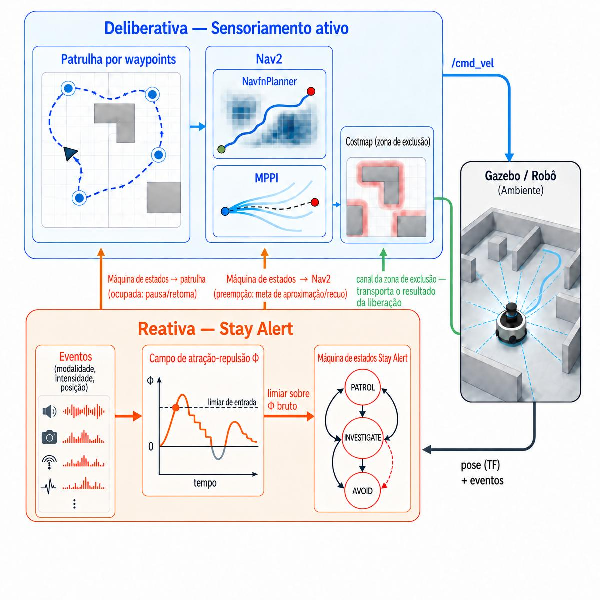
\includegraphics[width=0.9\textwidth]{figuras/architecture}
\caption{Arquitetura de duas camadas. A camada deliberativa (topo) conduz uma
patrulha por \textit{waypoints} através do Nav2 (NavfnPlanner $+$ MPPI), enviando
\texttt{/cmd\_vel} ao robô. A camada reativa (base, \textsc{Stay Alert}) converte
eventos percebidos no campo de atração/repulsão e executa a máquina de estados
finitos; ela preempta o Nav2 com uma meta de aproximação ou recuo e pausa ou retoma a
patrulha. O ambiente devolve pose (TF) e eventos.}
\label{fig:prop-arquitetura}
\end{figure}

\section{O Campo de Atração--Repulsão}
\label{sec:prop-campo}

A camada reativa é conduzida por um campo escalar $\Phi_t$ que agrega os eventos
sensoriais na localização do robô --- modalidade, intensidade e distância --- e
carrega o sinal da resposta: positivo para atração, negativo para repulsão. Ele é
função das observações correntes \emph{e} de duas memórias de canal com decaimento,
definidas adiante, de modo que é função do tempo, e não da observação instantânea
isolada. Ele não depende de qual ação é tomada. Escreve-se $\Phi$ por $\Phi_t$ onde o
índice temporal for dispensável:

\begin{equation}
\label{eq:prop-phi}
\Phi
\begin{cases}
> 0 & \text{atração (anomalia: aproximar)}\\
< 0 & \text{repulsão (risco: recuar)}\\
= 0 & \text{neutro (comportamento padrão de patrulha).}
\end{cases}
\end{equation}

\subsection{Intensidade Percebida e Fronteira de Detecção}

O campo é formado a partir de \emph{eventos} sensoriais. Um evento $e$ de modalidade
$m\in\{\text{térmica},\text{acústica},\text{risco}\}$ a uma distância $d$ do robô é
percebido dentro de um raio de detecção $R$ com intensidade

\begin{equation}
\label{eq:prop-intensidade}
i_e(d) = I_e\left(1 - \tfrac{1}{2}\,\frac{d}{R}\right), \qquad d \le R,
\end{equation}

sendo $I_e$ sua intensidade base. Esse perfil modela uma \emph{fronteira suave de
detecção}: o sensoriamento degrada linearmente com o alcance e não é reportado além
de $R$.

O degrau resultante em $d=R$ --- de $I_e/2$ para a ausência de evento --- é uma
descontinuidade real da intensidade percebida. Dois mecanismos do controlador
destinam-se a impedir que ela produza disparos repetidos: a histerese, com limiares
distintos de entrada e saída (Seção~\ref{sec:prop-stayalert}), e o compromisso, pois
uma vez comprometido um evento ele não é reselecionado até o fim do episódio.

\subsection{Canais com Memória e Precedência Categórica}

Cada modalidade possui um peso $w_m$ (com $w_{\text{risco}}<0$, para repulsão) e um
limiar de disparo $\theta_m$. O campo impõe \emph{segurança antes de inspeção} como
regra de \emph{precedência}, e não como disputa de magnitude: sempre que qualquer
evento repulsivo esteja acima do limiar e dentro do alcance, $\Phi$ assume seu valor
(negativo); apenas na ausência de risco o campo seleciona, entre os eventos de
atração concorrentes, o de maior magnitude.

Sejam $\mathcal{E}_{\mathcal{H}}$ e $\mathcal{E}_{\mathcal{A}}$ os conjuntos de
eventos de risco e de atração acima do limiar e dentro do alcance no passo corrente.
O evento governante e o campo são formados por \emph{dois acumuladores com
decaimento} --- um canal de risco $h\ge 0$ e um canal de atração com sinal $a$ ---
em vez de por uma única seleção instantânea. Escrevendo $c_e=w_{m(e)}\,i_e$ para a
contribuição com sinal do evento $e$, cada passo atualiza os canais por retenção de
máximo preservadora de magnitude:

\begin{align}
\label{eq:prop-canais}
h &\leftarrow \max\!\big(h,\ \textstyle\max_{e\in\mathcal{E}_{\mathcal{H}}}|c_e|\big),\\
a &\leftarrow c_{e^\star}\ \ \text{quando } |c_{e^\star}|>|a|\ \ (\text{retido, caso contrário}),
\end{align}

com $e^\star=\operatorname*{arg\,max}_{e\in\mathcal{E}_{\mathcal{A}}}|c_e|$ e empates
resolvidos pela menor identidade de evento. Uma vez por período de decaimento, ambos
os canais relaxam geometricamente e são zerados em um resíduo $\varepsilon$:

\begin{equation}
\label{eq:prop-decaimento}
h\leftarrow\lambda h,\qquad a\leftarrow\lambda a\quad(\text{zerado se abaixo de }\varepsilon).
\end{equation}

Cada acumulador é \emph{saturado no próprio lugar} na atualização ---
$h\in[0,\Phi_{\max}]$ e $a\in[-\Phi_{\max},\Phi_{\max}]$ ---, de modo que o valor
armazenado, e não apenas sua leitura, é limitado. O campo é então lido por
\emph{precedência categórica}:

\begin{equation}
\label{eq:prop-precedencia}
\Phi=-h\ \ \text{se } h>\varepsilon,\qquad
\Phi=a\ \ \text{caso contrário,}
\end{equation}

com decaimento $\lambda\in(0,1)$, resíduo $\varepsilon$ e período de decaimento
$T_d$. Quando o conjunto elegível \emph{próprio} de um canal está vazio em um passo,
esse canal é deixado ao decaimento da Equação~\eqref{eq:prop-decaimento} enquanto o
outro ainda pode ser atualizado por seus eventos.

Essa memória tem duas consequências que uma regra puramente instantânea não teria:

\begin{enumerate}
    \item um risco \emph{recentemente observado} continua governando o campo através
    de sua magnitude em decaimento, mesmo quando apenas uma atração está no alcance no
    passo corrente, até que $h$ caia abaixo de $\varepsilon$;
    \item um evento corrente mais fraco não sobrescreve um evento armazenado mais
    forte até que este último tenha decaído.
\end{enumerate}

Riscos são considerados primeiro, de sorte que um canal de risco acima de
$\varepsilon$ sempre governa o campo, independentemente de uma atração concorrente
mais forte: a disputa de magnitude decide apenas \emph{qual anomalia} aproximar,
nunca se preferir inspeção à segurança. Essa propriedade é verificada diretamente no
cenário de conflito da Seção~\ref{sec:res-conflito}.

\section{A Camada Reativa \textsc{Stay Alert}}
\label{sec:prop-stayalert}

A camada \textsc{Stay Alert} é uma máquina de estados finitos com três modos:
\textsc{Patrol}, \textsc{Investigate} (atração) e \textsc{Avoid} (repulsão),
sumarizados no Algoritmo~\ref{alg:stayalert} e na Figura~\ref{fig:prop-fsm}.

A repulsão tem prioridade sobre a atração --- segurança antes de inspeção --- a
partir de \emph{qualquer} estado: sempre que $\Phi \le -\theta_{\text{in}}$ e houver
pose de recuo disponível, o robô entra em \textsc{Avoid} e navega até a pose de
recuo, \emph{preemptando} uma \textsc{Investigate} em curso (desfecho
\emph{adiado}), sujeito a um curto período refratário $t_{\text{ref}}$ que impede
redisparo imediato enquanto a zona de exclusão deliberativa assume. Caso contrário, a
partir de \textsc{Patrol}, se $\Phi \ge \theta_{\text{in}}$ a camada compromete o
evento mais saliente no alcance e entra em \textsc{Investigate}, navegando até sua
pose de inspeção. Ao entrar em qualquer dos modos, a camada ativa uma marca de
\emph{ocupado} que pausa a patrulha e emite um marcador de evento com a identidade do
alvo.

\subsection{Controle e Crédito São Etapas Distintas}
\label{sec:prop-confirmacao}

Duas etapas devem ser mantidas separadas, porque somente a primeira atua sobre o
robô.

O \emph{controlador} encerra um episódio de \textsc{Investigate} quando a navegação
reativa \emph{tem sucesso} e esta se mantém por uma permanência comandada
$t_{\text{dwell}}$. Uma navegação abortada ou cancelada, ou o esgotamento de um
orçamento $t_{\max}$, encerra o episódio como \emph{falho}. Em qualquer das saídas
ele emite um evento com a identidade do alvo e o motivo.

O \emph{avaliador}, um nó separado, recebe esse evento e só então compara a pose do
robô com a posição \emph{verdadeira} do alvo: dentro de uma \emph{distância de
confirmação} --- a distância de parada acrescida de uma tolerância --- a anomalia é
creditada como \emph{inspecionada}; caso contrário, o episódio é registrado como
rejeição na confirmação.

A confirmação, portanto, jamais retroalimenta o comportamento: nenhum episódio é
prolongado ou abreviado por ela. É também uma aproximação: não se verifica
independentemente a distância de parada completa nem a orientação, tampouco a
persistência ao longo de toda a permanência, e a métrica é nomeada de acordo.

O episódio \emph{não} termina meramente porque $\Phi$ decaiu, o que previne oscilação
ao atravessar um ``vale'' de baixa saliência entre eventos. O modo \textsc{Avoid}
termina quando o risco deixa o alcance, $\Phi > -\theta_{\text{out}}$ (\emph{seguro}),
ou ao alcançar a pose de recuo (\emph{recuado}), e então arma o período refratário.

Uma anomalia é \emph{comprometida} no \emph{início} de sua investigação --- após o
que deixa de atrair, removendo a oscilação
\textsc{Patrol}$\leftrightarrow$\textsc{Investigate} que surge quando um
\textit{waypoint} fica próximo a uma anomalia --- e é contada como
\emph{inspecionada} apenas mediante chegada bem-sucedida confirmada. Episódios que
terminam como \emph{falho} ou \emph{adiado} são mantidos como desfechos distintos e
jamais contados como inspeções.

\subsection{A Zona de Exclusão Deliberativa}
\label{sec:prop-keepout}

Um risco \emph{sobre} a rota de patrulha não pode ser resolvido apenas por recuo
reativo, já que o \textit{waypoint} seguinte está além dele. Acrescenta-se, por isso,
uma expressão \emph{deliberativa} da repulsão: sempre que um risco é \emph{detectado}
dentro do alcance sensorial, sua posição \emph{percebida} é projetada como região de
exclusão \emph{persistente} no \textit{costmap} global, que o planejador então
contorna pelo restante da missão. Essa projeção é um canal de mapa acionado por
detecção --- não consequência de completar um recuo --- e usa a mesma informação
percebida que a camada reativa.

A entrega a esse canal é mais estreita do que ``suprimir $\Phi$'', e a distinção
importa. Ela ocorre na \emph{entrada} em \textsc{Avoid} e somente onde o canal de
exclusão está habilitado. O que ela bloqueia é a \emph{publicação} daquele risco como
evento: o risco deixa de ser reportado à camada reativa, de modo que novas
observações param de alimentar o acumulador de risco $h$. O valor já armazenado em
$h$ não é zerado --- ele decai pela Equação~\eqref{eq:prop-decaimento} até cair abaixo
de $\varepsilon$ --- e a região de exclusão permanece travada nesse meio-tempo, de
sorte que o planejador segue contornando a marca enquanto o sinal reativo se esvai. O
propósito é impedir que o robô oscile entre recuar e reaproximar enquanto o contorno é
percorrido.

Onde a zona de exclusão está \emph{desabilitada} --- o que ocorre em todo cenário fora
da rota --- não há entrega, o risco continua a ser publicado e a reobservação renova
$h$; a janela de supressão medida na Seção~\ref{sec:res-custo-precedencia} é,
portanto, mais longa do que o decaimento sozinho produziria.

\begin{figure}[htb]
\centering
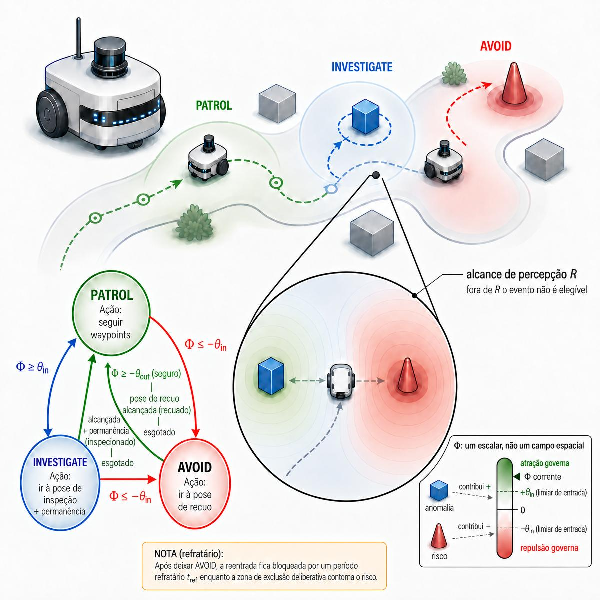
\includegraphics[width=0.9\textwidth]{figuras/stay_alert_fsm}
\caption{Máquina de estados \textsc{Stay Alert} e campo de atração--repulsão. Topo:
ao longo da patrulha o robô comuta para \textsc{Investigate} (aproximar-se de uma
anomalia) ou \textsc{Avoid} (recuar de um risco). Inferior esquerda: os três modos e
suas transições (limiares $\theta_{\text{in}},\theta_{\text{out}}$; desfechos
\emph{inspecionado}/\emph{esgotado}/\emph{seguro}/\emph{recuado}; a repulsão tem
prioridade). Inferior direita: o campo puxa em direção à atração e empurra para longe
da repulsão.}
\label{fig:prop-fsm}
\end{figure}

\begin{algorithm}[htb]
\caption{Camada reativa \textsc{Stay Alert} (por ciclo de controle)}
\label{alg:stayalert}
\begin{algorithmic}[1]
\STATE \textbf{entrada:} campo $\Phi$; evento selecionado $e^\star$ (mais saliente no
       alcance); limiares $\theta_{\text{in}},\theta_{\text{out}}$;
       $t_{\text{dwell}}, t_{\max}$; refratário $t_{\text{ref}}$
\STATE \textbf{Preempção de segurança} (um risco interrompe \emph{qualquer} estado):
\IF{o recuo reativo está habilitado \textbf{e} modo $\ne$ \textsc{Avoid}
    \textbf{e} $\Phi \le -\theta_{\text{in}}$
    \textbf{e} pose de recuo disponível \textbf{e} $t \ge t_{\text{avoid}}$}
  \IF{modo $=$ \textsc{Investigate}}
     \STATE sair (\emph{adiado por risco}); liberar alvo $e^\star$
  \ENDIF
  \STATE entrar em \textsc{Avoid}; pausar patrulha; enviar meta de recuo
  \IF{a zona de exclusão deliberativa está habilitada}
     \STATE \emph{entregar o risco à zona de exclusão}: cessar sua publicação à
            camada reativa, de modo que nenhuma nova observação alimente o canal de
            risco; o valor armazenado é mantido e deixado a decair
  \ENDIF
\ELSIF{modo $=$ \textsc{Patrol}}
  \IF{$\Phi \ge \theta_{\text{in}}$ \textbf{e} pose de inspeção disponível}
     \STATE comprometer alvo $e^\star$ (por identidade); entrar em
            \textsc{Investigate}; pausar patrulha; enviar meta de aproximação
  \ENDIF
\ELSIF{modo $=$ \textsc{Investigate}}
  \IF{navegação \textbf{bem-sucedida} \textbf{e} permanência $\ge t_{\text{dwell}}$}
     \STATE sair (\emph{inspecionado}); retomar patrulha
  \ELSIF{decorrido $\ge t_{\max}$ \textbf{ou} navegação abortada/cancelada}
     \STATE sair (\emph{falho}); retomar patrulha
  \ENDIF
\ELSIF{modo $=$ \textsc{Avoid}}
  \IF{$\Phi > -\theta_{\text{out}}$ \textbf{ou} pose de recuo alcançada}
     \STATE sair (\emph{seguro}/\emph{recuado});
            $t_{\text{avoid}} \gets t + t_{\text{ref}}$; retomar patrulha
  \ELSIF{decorrido $\ge t_{\max}$}
     \STATE sair (\emph{esgotado});
            $t_{\text{avoid}} \gets t + t_{\text{ref}}$; retomar patrulha
  \ENDIF
\ENDIF
\end{algorithmic}
\end{algorithm}

\section{Sensoriamento Ativo e Abstração de Eventos}
\label{sec:prop-sensoriamento}

A patrulha realiza o sensoriamento ativo ao conduzir os sensores ao longo da rota; a
pose do robô usada pela camada reativa é tomada no referencial do \emph{mapa} (via a
árvore TF), de modo que eventos, poses e o mapa estático sejam mutuamente
consistentes.

Dado um evento na posição $\bm{e}$ e o robô em $\bm{p}$, com direção unitária
$\hat{\bm{u}}=(\bm{p}-\bm{e})/\lVert\bm{p}-\bm{e}\rVert$, o modo
\textsc{Investigate} mira uma pose de inspeção a uma distância de parada $\rho$,
voltada para o evento,
$\bm{p}_{\text{insp}}=\bm{e}+\rho\,\hat{\bm{u}}$, enquanto \textsc{Avoid} mira uma
pose de recuo além do raio de detecção e voltada para o lado oposto,
$\bm{p}_{\text{ret}}=\bm{e}+(R+\Delta)\,\hat{\bm{u}}$. Eventos de atração são
comprometidos uma única vez, após o que deixam de atrair; riscos são persistentes.

\section{Sobre a Atualização de Valor}
\label{sec:prop-atualizacao}

O mesmo campo $\Phi$ pode ser escrito como termo adicional em uma atualização de
valor tabular, na forma

\begin{equation}
\label{eq:prop-bellman}
Q(s,a) \leftarrow Q(s,a) + \alpha\,\delta + \eta\,\Phi,
\end{equation}

sendo $\delta$ o erro de diferença temporal usual, $\alpha$ a taxa de aprendizado e
$\eta$ o peso do termo afetivo.

É preciso ser inequívoco quanto ao estatuto dessa formulação neste trabalho. A tabela
de valor \emph{não} seleciona as ações executadas: o comportamento imediato é
governado pelos limiares sobre o campo bruto $\Phi$ e pela máquina de estados do
Algoritmo~\ref{alg:stayalert}, e o movimento provém das metas enviadas ao Nav2/MPPI.
Em consequência, a varredura sobre $\eta$ relatada na literatura associada a este
trabalho constitui análise \emph{numérica da tabela de valor}, e não demonstração de
robustez comportamental --- e é assim que ela é apresentada.

%% Acrescentado em 12/11/2026. O estatuto teorico do termo aditivo precisa estar
%% declarado aqui, onde a equacao aparece, e nao so na conclusao: e a primeira coisa
%% que um leitor de aprendizado por reforco verifica.
Cabe ser igualmente inequívoco quanto ao estatuto \emph{teórico} do termo aditivo. O
campo $\Phi$ \emph{não} está formulado como termo potencial no sentido de
\citeonline{ng1999}, isto é, não assume a forma
$F(s,a,s')=\gamma\,\Phi(s')-\Phi(s)$ exigida para que a transformação preserve a
política ótima. O campo é aditivo, variante no tempo, sujeito a decaimento e
dependente dos eventos observados, de modo que \emph{nenhuma garantia de invariância
de política} se aplica à Equação~\eqref{eq:prop-bellman}, e nenhuma é reivindicada
nesta tese. Sob taxa de aprendizado $\alpha$ fixa, o incremento $\eta\Phi$ é,
ademais, representável como uma componente adicional de recompensa, à maneira de
outras abordagens que acoplam campos potenciais a aprendizado
\cite{zhang2023apf}: não há, portanto, novidade a reivindicar sobre o aumento de
recompensa no plano formal, e a contribuição desta tese não se localiza aí. Daí
também decorre a escolha de vocabulário mantida em todo o documento --- relata-se
\emph{estabilidade dos incrementos} nas simulações avaliadas, e não convergência.

Registra-se a formulação aqui como \emph{nota de projeto}, isto é, como caminho
previsto para uma política aprendida futura, e não como componente validado da
arquitetura avaliada. Para que esse caminho não ficasse apenas enunciado, ele foi
levado a funcionar em um braço separado: a Seção~\ref{sec:res-qdriven} relata um
\textit{baseline} em que uma tabela $Q$, treinada com recompensa aumentada por
$\Phi$, \emph{seleciona} a ação executada, medido contra o método nos três
cenários. O Capítulo~\ref{cap:resultados} relata o resíduo completo
$|\alpha\delta+\eta\Phi|$ como evidência de que os incrementos permanecem limitados
nas simulações avaliadas --- o que atesta estabilidade dos incrementos, e não
convergência, e muito menos que a atualização governe o comportamento.


% ----------------------------------------------------------
% Avaliação Experimental
% ----------------------------------------------------------
\chapter{Avaliação Experimental}
\label{cap:avaliacao}

Este capítulo descreve o ambiente de simulação, os cenários, a matriz experimental e
as métricas empregadas na avaliação da arquitetura do Capítulo~\ref{cap:proposta}.
Os resultados obtidos são relatados no Capítulo~\ref{cap:resultados}.

\section{Ambiente de Simulação e Pilha de \textit{Software}}
\label{sec:setup-ambiente}

Os experimentos rodam sobre ROS~2 Humble com Gazebo Fortress (Ignition Gazebo~6)
como simulador de física, interligados por \texttt{ros\_gz}. O robô é uma plataforma
de tração diferencial (\emph{inspector\_bot}) com sensor planar de distância de
$360^\circ$.

O planejamento global de caminho usa a pilha Nav2 com o planejador global
\emph{NavfnPlanner} e um controlador \textit{Model Predictive Path Integral} (MPPI)
para seguimento de caminho (modelo de movimento diferencial, frequência de controle
de $20$~Hz) sobre um mapa de ocupação \emph{estático}. A pilha Nav2 é configurada com
\textit{Adaptive Monte Carlo Localization} (AMCL), mas nestes experimentos a
transformada \texttt{map}$\rightarrow$\texttt{odom} é mantida fixa, de modo que a
pose do robô é exata e a deriva de localização não é modelada; a pose usada pelos nós
de percepção e de métricas é, portanto, a transformada verdadeira no referencial do
mapa, e não uma estimativa do AMCL.

Os \textit{costmaps} usam raio do robô de $0{,}25$~m, raio de inflação de $0{,}55$~m
e fator de escala de custo de $3{,}0$; a tolerância de meta é de $0{,}25$~m.

\subsection{O Mundo Simulado}

O mundo modela uma subestação simplificada (Figura~\ref{fig:setup-mundo}): um
transformador de potência ($3{\times}2{\times}1{,}5$~m em $(10,10)$), um disjuntor
($1{\times}1{\times}2$~m em $(-5,5)$), um barramento
($8{\times}0{,}3{\times}0{,}3$~m em $(0,15)$) e uma cerca perimetral de
$50{\times}50$~m, sobre um plano de solo. O mapa de ocupação estático
($1040{\times}1040$ células a $0{,}05$~m/célula) é alinhado ao referencial do mundo,
de sorte que \textit{waypoints} em coordenadas do mundo servem diretamente como metas
de navegação.

A patrulha deliberativa visita cinco \textit{waypoints} (em metros): $(13,-8)$,
$(13,10)$, $(0,11)$, $(-8,5)$ e um retorno em $(-10,-10)$.

\begin{figure}[htb]
\centering
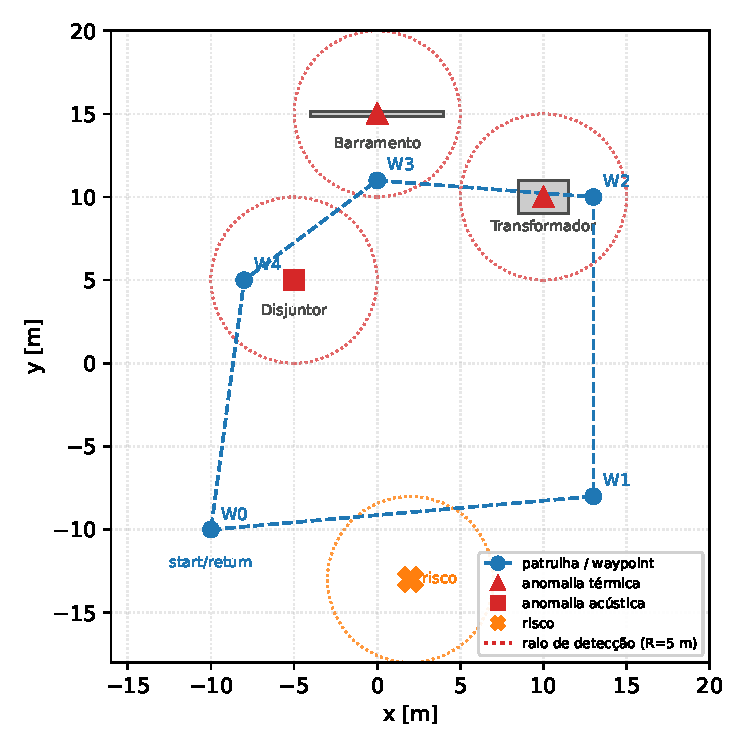
\includegraphics[width=0.85\textwidth]{figuras/world_map}
\caption{Cenário da subestação (padrão): equipamentos (cinza), os cinco
\textit{waypoints} de patrulha W0--W4 e a ronda (tracejada), as anomalias de atração
(térmica $\triangle$, acústica $\square$) e o risco ($\times$), cada qual com seu
raio de detecção $R=5$~m (pontilhado). Coordenadas em metros, referencial do mundo.}
\label{fig:setup-mundo}
\end{figure}

\section{Eventos Simulados e Cenários}
\label{sec:setup-eventos}

Conforme a Seção~\ref{sec:prop-sensoriamento}, a saída da percepção é abstraída como
eventos. Definem-se os seguintes cenários:

\begin{description}
    \item[\texttt{default}] Três anomalias de atração --- um evento térmico no
    transformador $(10,10)$, um evento térmico no barramento $(0,15)$ e um evento
    acústico no disjuntor $(-5,5)$ --- e um risco persistente (repulsão) ao lado da
    primeira perna de patrulha, em $(2,-13)$.

    \item[\texttt{adverse}] Adensa as anomalias em aglomerados (cinco anomalias: duas
    próximas ao transformador, duas próximas ao disjuntor, mais o barramento), de modo
    que múltiplos eventos caiam simultaneamente dentro do raio sensorial e a camada
    tenha de arbitrar entre eles; o risco permanece inalterado.

    \item[\texttt{route-hazard}] Mantém as três anomalias padrão mas move o risco
    \emph{para cima} da primeira perna de patrulha, em $(1{,}5,-9)$ --- bloqueando
    diretamente o caminho ao \textit{waypoint} seguinte ---, de sorte que um recuo
    puramente reativo não possa resolvê-lo sem desviar a rota. Aqui o risco detectado
    é também projetado, em sua posição \emph{percebida}, como zona de exclusão
    persistente no \textit{costmap} global.

    \item[\texttt{conflict}] Mantém as três anomalias padrão e colocaliza, na posição
    do risco padrão $(2,-13)$, uma anomalia acústica \emph{forte} ($I_e=0{,}95$,
    $|w\,I_e|=1{,}14$) com um risco \emph{mais fraco} ($I_e=0{,}70$,
    $|w\,I_e|=1{,}05$): a atração é a mais saliente das duas, de modo que uma regra
    puramente de magnitude preferiria a inspeção, ao passo que a regra de precedência
    deve disparar \textsc{Avoid}.

    \item[\texttt{dyn-hazard}] Um risco colocalizado com uma anomalia permanece
    \emph{inativo} até que o robô --- já comprometido com sua inspeção --- se aproxime
    a $3$~m, ponto em que o ambiente o ativa. É o único cenário em que o risco
    \emph{emerge} durante uma investigação.

    \item[\texttt{marginal}] Um risco de intensidade elegível mínima ao lado da
    primeira perna de patrulha, junto a uma anomalia acústica legítima de intensidade
    $0{,}95$ posicionada a $4{,}3$~m dele, para medir o custo da precedência
    categórica na faixa em que o risco governa o campo sem disparar recuo.
\end{description}

O raio de detecção é $R=5$~m, a distância de parada de inspeção é $\rho=2$~m e a
margem de recuo é $\Delta=1{,}5$~m.

\section{Matriz Experimental}
\label{sec:setup-matriz}

A camada reativa é avaliada contra uma linha de base fixa e uma linha de base de
campo potencial artificial, ao longo de uma varredura de $\eta$, de uma ablação com
$\eta=0$, de um cenário adverso, de um risco colocado sobre a rota e de perturbações
de ruído de percepção (Tabela~\ref{tab:setup-matriz}). Cada configuração é executada
$n=10$ vezes, sem interface gráfica e com limite de $600$~s por execução.

%% Acrescentado em 13/11/2026: o limite de execucao e de RELOGIO DE PAREDE, enquanto a
%% duracao de missao relatada e de relogio simulado. Sem essa distincao a KOb aparece
%% com 627 s sob um limite de 600 s, o que parece contradicao e nao e.
Esse limite é de \emph{relógio de parede} e governa o \textit{script} de execução, que
encerra o processo quando a missão não atinge o estado \texttt{COMPLETE} dentro da
janela. A duração de missão relatada no Capítulo~\ref{cap:resultados} é medida no
\emph{relógio simulado}, a partir do início da missão e já descontada a subida dos nós.
Os dois relógios não coincidem: sobre as execuções concluídas, a razão mediana entre o
relógio simulado e o de parede é de $1{,}12$ (faixa de $1{,}11$ a $1{,}15$), de sorte que
o limite de $600$~s de parede corresponde a aproximadamente $674$~s de relógio simulado,
ou cerca de $627$~s de missão. É por isso que uma configuração interrompida pelo limite
pode exibir duração de missão superior a $600$~s: o valor relatado é o do relógio
simulado no instante da interrupção, e não uma missão concluída.

\begin{table}[htb]
\centering
\caption{Matriz experimental ($10$ execuções tentadas por configuração).
\emph{Rec.} é o recuo reflexivo e \emph{ZE} a zona de exclusão deliberativa; ambos
são parâmetros de lançamento, listados aqui porque a entrega descrita na
Seção~\ref{sec:prop-keepout} só ocorre onde a zona de exclusão está habilitada. A
zona de exclusão está ligada apenas onde um risco se encontra sobre a rota de
patrulha ou emerge durante uma investigação; em todo cenário fora da rota ela está
desligada, e a reobservação pode seguir renovando o canal de risco. As linhas HEU,
HEU-sel e Q-driven abrangem três cenários cada, o que as desdobra em três rótulos de
execução; as demais correspondem a um rótulo cada. São, portanto, $32$ pares
configuração--cenário e $320$ execuções tentadas, censadas na
Tabela~\ref{tab:setup-censo}. As três linhas HAZ varrem o limiar de elegibilidade de
modalidade $\theta_{\mathcal{H}}$ (Seção~\ref{sec:res-sens-limiar}) e as duas linhas
HYS variam o par entrada/saída da histerese contra a referência $0{,}45/0{,}25$
(Seção~\ref{sec:res-histerese}); ambas as varreduras mantêm \textsc{Stay Alert} ativa
com $\eta=0{,}5$.}
\label{tab:setup-matriz}
\footnotesize
\begin{tabular}{llcccl}
\hline
\textbf{Exp.} & \textbf{Camada reativa} & $\bm{\eta}$ & \textbf{Rec.} &
\textbf{ZE} & \textbf{Cenário (\#anom./risco)}\\
\hline
E1  & nenhuma                      & ---   & ---        & ---        & \texttt{default} (3/1)\\
E0  & Stay Alert (ablação)         & 0     & \checkmark & ---        & \texttt{default} (3/1)\\
E2  & Stay Alert                   & 0,3   & \checkmark & ---        & \texttt{default} (3/1)\\
E3  & Stay Alert                   & 0,5   & \checkmark & ---        & \texttt{default} (3/1)\\
E4  & Stay Alert                   & 0,8   & \checkmark & ---        & \texttt{default} (3/1)\\
E5  & Stay Alert                   & 0,5   & \checkmark & ---        & \texttt{adverse} (5/1)\\
APF & campo potencial              & ---   & \checkmark & ---        & \texttt{default} (3/1)\\
RHM & Stay Alert                   & 0,5   & \checkmark & \checkmark & \texttt{route-hazard} (3/1)\\
RHB & nenhuma                      & ---   & ---        & ---        & \texttt{route-hazard} (3/1)\\
N1  & Stay Alert (ruído moderado)  & 0,5   & \checkmark & ---        & \texttt{default} (3/1)\\
N2  & Stay Alert (ruído alto)      & 0,5   & \checkmark & ---        & \texttt{default} (3/1)\\
CONF& Stay Alert                   & 0,5   & \checkmark & ---        & \texttt{conflict} (4/1)\\
KOa & somente zona de exclusão     & 0,5   & ---        & \checkmark & \texttt{route-hazard} (3/1)\\
KOb & somente recuo                & 0,5   & \checkmark & ---        & \texttt{route-hazard} (3/1)\\
KOF & patrulha fixa com zona excl. & ---   & ---        & \checkmark & \texttt{route-hazard} (3/1)\\
DHa & recuo $+$ zona de exclusão   & 0,5   & \checkmark & \checkmark & \texttt{dyn-hazard} (1/1)\\
DHb & somente zona de exclusão     & 0,5   & ---        & \checkmark & \texttt{dyn-hazard} (1/1)\\
HEU & supervisor heurístico        & ---   & \checkmark & ---        & \texttt{default}/\texttt{conflict}/\texttt{adverse}\\
HEU-sel & seleção por proximidade  & 0,5   & \checkmark & ---        & \texttt{default}/\texttt{conflict}/\texttt{adverse}\\
CM  & Stay Alert                   & 0,5   & \checkmark & ---        & \texttt{marginal} (4/1)\\
%% Acrescentado em 13/11/2026: bloco exploratorio de RL comportamental.
Q-driven & $Q$ greedy pre-treinada      & ---   & \checkmark & ---        & \texttt{default}/\texttt{conflict}/\texttt{adverse}\\
%% Acrescentadas em 13/11/2026: as cinco varreduras executadas e relatadas nas
%% Secoes~\ref{sec:res-sens-limiar} e~\ref{sec:res-histerese} faltavam nesta matriz,
%% embora a introducao as mencionasse e os dados existissem. Sem elas o censo de
%% execucoes nao fechava.
HAZ20 & $\theta_{\mathcal{H}}=0{,}20$  & 0,5   & \checkmark & ---        & \texttt{conflict} (4/1)\\
HAZ30 & $\theta_{\mathcal{H}}=0{,}30$  & 0,5   & \checkmark & ---        & \texttt{conflict} (4/1)\\
HAZ40 & $\theta_{\mathcal{H}}=0{,}40$  & 0,5   & \checkmark & ---        & \texttt{conflict} (4/1)\\
HYSnar & histerese $0{,}45/0{,}35$     & 0,5   & \checkmark & ---        & \texttt{default} (3/1)\\
HYSoff & histerese $0{,}55/0{,}35$     & 0,5   & \checkmark & ---        & \texttt{default} (3/1)\\
\hline
\end{tabular}
\end{table}

%% Secao acrescentada em 13/11/2026 para fechar o censo de execucoes. O problema que
%% ela resolve: a introducao declarava vinte configuracoes, a matriz listava vinte e
%% uma linhas, os dados em disco tinham trinta e dois rotulos, e a Secao 6.1.1 falava
%% de 160 tentativas -- numero correto para a matriz do artigo, nao para a desta tese.
%% Todos os totais abaixo saem do mesmo manifesto, gerado por
%% src/tese_nav/scripts/gerar_manifesto.py a partir dos CSVs e dos logs de bateria.
\section{Censo de Execuções}
\label{sec:setup-censo}

Todos os totais de execução citados nesta tese derivam de um único manifesto,
reconstruído a partir dos arquivos de métrica por execução e dos \textit{logs} de
bateria, com um registro por execução: rótulo, cenário, semente, horário de início,
desfecho do \textit{script} de execução, critério de validade, duração e arquivo de
origem. O manifesto é regenerado por \texttt{gerar\_manifesto.py} e acompanha o pacote
de reprodução.

A Tabela~\ref{tab:setup-censo} separa as quatro contagens que não devem ser somadas
entre si.

\begin{table}[htb]
\centering
\caption{Censo das execuções analisadas. O critério de validade é o de movimento
(distância percorrida $>1$~m): uma execução imóvel é um desfecho de confiabilidade de
inicialização, não um resultado de navegação, e é relatada separadamente na
Seção~\ref{sec:res-validade}. ``Interrompida pelo limite'' designa execução válida que
não atingiu \texttt{COMPLETE} dentro dos $600$~s de relógio de parede, de sorte que sua
duração é um limite inferior e não um tempo de missão.}
\label{tab:setup-censo}
\footnotesize
\begin{tabular}{lr}
\hline
\textbf{Contagem} & \textbf{Valor}\\
\hline
Pares configuração--cenário                     & $32$\\
Execuções tentadas ($10$ por par)               & $320$\\
Execuções válidas                               & $311$\\
\quad das quais concluíram a missão             & $302$\\
\quad das quais interrompidas pelo limite       & $9$ (todas KOb)\\
Execuções imóveis (falha de inicialização)      & $9$\\
Confiabilidade de partida por tentativa         & $311/320 = 97{,}2\%$\\
\hline
\end{tabular}
\end{table}

As $320$ execuções distribuem-se pelos seis cenários como $130$ em \texttt{default},
$70$ em \texttt{conflict}, $50$ em \texttt{route-hazard}, $40$ em \texttt{adverse},
$20$ em \texttt{dyn-hazard} e $10$ em \texttt{marginal}. Cada configuração usa as
sementes $1$ a $10$, uma por execução, e o manifesto registra a semente de cada uma.

As nove execuções imóveis distribuem-se por oito configurações --- APF, HEUc, HEUd,
HYSoff, KOb, N2 e RHM com uma cada, DHa com duas ---, de modo que nenhuma configuração
fica com menos de oito execuções válidas. As nove execuções interrompidas pelo limite
são \emph{todas} da configuração KOb, que não encerra a missão por construção, conforme
se analisa na Seção~\ref{sec:res-ablacao}; em todas as demais configurações, toda
execução válida atingiu \texttt{COMPLETE}.

Três contagens \emph{não} entram nesse censo, para que não sejam confundidas com
execuções da matriz:

\begin{enumerate}
    \item \textbf{Baterias anteriores descartadas.} Os \textit{logs} registram $479$
    lançamentos ao todo, contra as $320$ execuções analisadas. O excedente são baterias
    anteriores substituídas --- uma bateria contaminada por nó órfão entre execuções, um
    bloco interrompido pela metade e um ensaio de regressão para o portão de reúso ---,
    preservadas em diretórios separados em vez de apagadas. Uma execução descartada não
    é uma execução da matriz, e nenhuma delas entra em qualquer tabela de resultados.

    \item \textbf{Controles reutilizados.} Onde um bloco posterior se compara a um
    controle já executado, o controle é \emph{reutilizado}, não reexecutado: reusar um
    controle não cria execução nova. É o caso da configuração E3, que serve de controle
    do método em \texttt{default} para mais de um contraste.

    \item \textbf{Reanálises de registros existentes.} Reavaliar um limiar de métrica
    sobre os mesmos \textit{logs} --- como a reanálise do limiar de confirmação de
    inspeção da Seção~\ref{sec:res-ruido} --- é reanálise, não execução adicional.
\end{enumerate}

\section{Métricas}
\label{sec:setup-metricas}

Registram-se, por execução:

\begin{description}
    \item[Anomalias inspecionadas] Número de alvos de atração com chegada
    bem-sucedida \emph{confirmada}, no sentido da Seção~\ref{sec:prop-confirmacao}.
    Episódios encerrados como \emph{falho} ou \emph{adiado} não são contados.

    \item[Desvios de rota] Número de preempções do \textit{waypoint} corrente pela
    camada reativa. Como mostra a Seção~\ref{sec:res-custo-precedencia}, essa métrica
    é sensível à \emph{posição} do limiar de entrada, e não é contagem intrínseca do
    cenário.

    \item[Esquivas de risco (recuos)] Número de entradas no modo \textsc{Avoid}.

    \item[Distância mínima ao risco] Mínimo, ao longo da missão, da distância entre a
    posição verdadeira do robô e a posição verdadeira do risco. É medida
    independentemente de $\Phi$, de modo que suprimir o sinal reativo não a infla.

    \item[Tempo mínimo até a colisão] Mínimo da razão entre distância e velocidade
    radial de aproximação.

    \item[Colisões] Número de entradas em uma região de contato de $0{,}5$~m
    centro a centro. Com raio do robô de $0{,}25$~m configurado no planejador, essa
    distância deixa $0{,}25$~m entre a borda do robô e o ponto de risco. Trata-se de
    distância a um risco representado como \emph{ponto}; o equipamento que ele
    representa tem extensão finita, de sorte que não é afastamento de uma superfície
    física.

    \item[Tempo abaixo do afastamento] Tempo acumulado abaixo de uma faixa de $2$~m.
    Esse valor é limiar \emph{diagnóstico} adotado para medir exposição nesta
    avaliação; o estudo não declara requisito de afastamento mínimo, de modo que
    transitar abaixo dele não é violação de requisito, mas exposição que se relata.

    \item[Duração da missão e distância percorrida] Tempo total e comprimento de
    caminho até o encerramento da ronda.

    \item[Tempo de investigação] Tempo \emph{total} por execução passado em
    \textsc{Investigate}, e não média por episódio --- de modo que uma configuração
    que nunca investiga contribui com um $0$ bem definido, em vez de média
    indefinida.

    \item[Resíduo de atualização] $|\alpha\delta+\eta\Phi|$ completo, registrado como
    evidência de que os incrementos da Equação~\eqref{eq:prop-bellman} permanecem
    limitados. Conforme a Seção~\ref{sec:prop-atualizacao}, isso atesta estabilidade
    dos incrementos, não convergência nem governo do comportamento.
\end{description}

\section{Hiperparâmetros}
\label{sec:setup-hiper}

A Tabela~\ref{tab:setup-hiper} resume os hiperparâmetros do método e da simulação.

\begin{table}[htb]
\centering
\caption{Hiperparâmetros do método e da simulação.}
\label{tab:setup-hiper}
\footnotesize
\begin{tabular}{lll}
\hline
\textbf{Grupo} & \textbf{Parâmetro} & \textbf{Valor}\\
\hline
Atualização de valor & taxa de aprendizado $\alpha$ & 0,1\\
(Seção~\ref{sec:prop-atualizacao}) & desconto $\gamma$ & 0,95\\
          & peso afetivo $\eta$ & 0,3 / 0,5 / 0,8\\
          & tamanho de célula $\delta$; \textit{buckets} $B$ & 1,0~m; 4\\
          & recompensa de progresso $r_{\text{prog}}$ & 1,0\\
Campo $\Phi$ & pesos (térm./acúst./risco) & 1,0 / 1,2 / $-1{,}5$\\
          & limiares $\theta_m$ & 0,4 / 0,3 / 0,3\\
          & decaimento $\lambda$; saturação $\Phi_{\max}$ & 0,85; 2,0\\
          & período de decaimento $T_d$; resíduo $\varepsilon$ & 1~s; $10^{-3}$\\
\textsc{Stay Alert} & entrada $\theta_{\text{in}}$; saída $\theta_{\text{out}}$ & 0,45; 0,25\\
          & permanência $t_{\text{dwell}}$; orçamento $t_{\max}$ & 3~s; 40~s\\
          & refratário $t_{\text{ref}}$ & 8~s\\
Avaliador & distância de confirmação (métrica) & 3,3~m\\
Zona de exclusão & raio de projeção; raio do disco & 5~m; 1,2~m\\
Base APF  & distância de parada; orçamento & 1,8~m; 30~s\\
          & ganhos $k_{\text{att}}$/$k_{\text{rep}}$/$k_{\text{obs}}$ & 1,5 / 4,0 / 0,6\\
          & disparo; saída (magnitude de força) & 0,15; 0,08\\
          & refratário pós-recuo & 12~s\\
Eventos   & raio $R$; distância de parada $\rho$ & 5~m; 2~m\\
          & margem de recuo $\Delta$ & 1,5~m\\
\hline
\end{tabular}
\end{table}

\section{Reprodutibilidade}
\label{sec:setup-repro}

O código completo, o mundo simulado, os arquivos de lançamento, o executor de
bateria e o \textit{script} de análise estão publicamente
disponíveis\footnote{\texttt{github.com/voidmmn/tese\_react\_nav}}. \textit{Scripts}
de instalação configuram ROS~2 Humble, Gazebo Fortress e Nav2; um \textit{script} de
lote executa a matriz completa e grava um arquivo CSV por execução, e o
\textit{script} de análise produz a tabela-resumo e os testes estatísticos relatados
no Capítulo~\ref{cap:resultados}.

Os valores por execução, com sementes e desfechos individuais, são publicados junto
ao código, de modo que os denominadores de toda taxa relatada possam ser conferidos
em vez de aceitos por confiança.


% ----------------------------------------------------------
% Resultados e Discussão
% ----------------------------------------------------------
\chapter{Resultados e Discussão}
\label{cap:resultados}

Este capítulo apresenta a avaliação experimental da arquitetura descrita no
Capítulo~\ref{cap:proposta}. Os resultados aqui relatados são os mesmos que
sustentam o artigo publicado no periódico \textit{IEEE Access}, aceito em novembro
de 2026, e foram obtidos integralmente em simulação, no ambiente descrito na
Seção~\ref{sec:setup-ambiente}.

Antes de qualquer número, convém fixar o que esta avaliação pode e o que não pode
sustentar. A percepção é abstraída em eventos-oráculo: o simulador publica
modalidade, intensidade e posição de cada evento sem incerteza associada, e a
transformada de localização é fixa. Em consequência, os resultados falam da
\emph{lógica de decisão} da arquitetura --- quando desviar, de que se afastar, o que
inspecionar primeiro --- e não de um sistema pronto para implantação. A
Seção~\ref{sec:res-ruido} relaxa parcialmente a primeira dessas idealizações
injetando ruído na percepção, e a Seção~\ref{sec:res-ameacas} enumera o que
permanece fora do alcance do estudo.

\section{Protocolo de Análise}
\label{sec:res-protocolo}

Relatam-se os valores finais, por execução, de cada métrica, agregados sobre até
$n=10$ execuções por configuração. Vários desfechos são contagens limitadas, com
variância nula ou quase nula, para as quais as premissas de um teste $t$ paramétrico
não se sustentam. As comparações entre grupos empregam, portanto, testes livres de
distribuição: o $U$ de Mann--Whitney, cujo $p$ é calculado caso a caso --- a
distribuição \emph{exata} de $U$ para amostras sem empates com $n_1+n_2\le20$
(todos os pares aqui), o $p$ exato de permutação bilateral para braços constantes
completamente separados, e a aproximação normal corrigida para empates apenas quando
há empates. Cada comparação é acompanhada do tamanho de efeito $\delta$ de Cliff e de
intervalos de confiança \textit{bootstrap} de $95\%$. Equivalência, quando
mencionada, é avaliada por dois testes unilaterais (TOST); taxas de sucesso por
missão são relatadas com intervalos de Wilson.

\subsection{Execuções Válidas e Confiabilidade de Inicialização}

Execuções em que a plataforma não se moveu (distância percorrida $\approx 0$)
constituem um desfecho de confiabilidade de inicialização, não um resultado de
navegação. Das $160$ execuções tentadas, $154$ atenderam ao critério de movimento
para análise comportamental e $6$ permaneceram imóveis. O critério observável e
publicado para essas seis é a \emph{imobilidade} --- o critério de distância do
analisador; a maioria acumula relógio de missão sem qualquer deslocamento. Lemos
esse padrão como consistente com uma falha de \emph{inicialização} (o contêiner de
navegação não subindo o robô), mas não certificamos essa causa de infraestrutura a
partir dos \textit{logs} brutos publicados.

Relatam-se duas visões complementares, em vez de agregá-las:

\begin{enumerate}
    \item desempenho \emph{condicional à inicialização bem-sucedida}, calculado
    sobre as execuções válidas ($n=8$ a $10$ por configuração);
    \item confiabilidade de partida \emph{por tentativa} ($154/160 = 96{,}25\%$).
\end{enumerate}

As execuções imóveis \emph{não} são promediadas nas métricas comportamentais --- sua
distância nula e inspeção nula enviesariam médias e taxas --- e são relatadas
separadamente como desfecho de confiabilidade. Os valores por execução, com
sementes e desfechos individuais, são publicados junto ao código.

\subsection{Alegações Primárias e Exploratórias}
\label{sec:res-familias}

A fronteira entre alegações confirmatórias e exploratórias é fixada aqui e marcada
em cada afirmação, e não apenas nas tabelas. É preciso ser exato quanto a que parte
da família foi fixada antecipadamente.

Os três \emph{contrastes} foram especificados antes de a nova bateria gravar seu
primeiro arquivo de resultado: a camada proposta contra a heurística genérica e
contra a variante de seleção de um fator, no cenário \texttt{default}; e a ablação
somente-\textit{keep-out} contra a patrulha fixa portando o mesmo \textit{keep-out}
(KOa \textit{vs.} KOF), no risco sobre a rota. O que o registro estabelece é
exatamente isso: o plano de análise publicado carrega os três contrastes em um
\textit{commit} que precede a primeira execução arquivada em cerca de uma hora. Não
se alega mais do que a ordenação que esse \textit{commit} demonstra.

O \emph{conjunto de desfechos} sobre os quais cada contraste é avaliado \emph{não}
foi declarado antecipadamente: os cinco aqui relatados --- anomalias inspecionadas,
distância mínima ao risco, duração da missão, recuos e tempo de investigação ---
foram fixados após as execuções. Chamamos esses quinze testes de \emph{família de
comparação primária com desfechos especificados retrospectivamente}, e não de
família confirmatória: a correção de Holm trata a multiplicidade \emph{dentro da
família tal como relatada}, mas não torna prospectiva a escolha dos desfechos, e
registro público é questão distinta, que tampouco se alega. O conjunto completo é
tabulado sem omissão de teste, de modo que o denominador possa ser conferido em vez
de aceito por confiança.

Todo o restante --- os cenários \texttt{conflict} e \texttt{adverse}, as varreduras
de limiar e de histerese, a configuração de risco marginal e toda reanálise de
execuções previamente gravadas --- é \emph{exploratório}, é relatado com $p$ não
corrigido e é rotulado como exploratório na própria frase que o enuncia.

\section{Detecção e Comportamento de Inspeção}
\label{sec:res-inspecao}

O resultado central é que a camada reativa converte uma patrulha de cobertura em um
comportamento de inspeção. A Tabela~\ref{tab:res-principal} consolida as métricas
por configuração.

A linha de base fixa (E1) inspeciona \emph{nenhuma} anomalia: percorre a ronda e
nunca se desvia ($0{,}0\pm0{,}0$). Com a camada \textsc{Stay Alert}, o robô
inspeciona \emph{todas as três} anomalias em toda execução válida do cenário padrão,
em qualquer ajuste de $\eta$, inclusive na ablação $\eta=0$ (E0--E4 todas em
$3{,}0\pm0{,}0$; $\delta$ de Cliff igual a $1$, permutação exata
$p=1{,}1\times10^{-5}$ contra E1). Essa completude se degrada sob ruído alto de
percepção (Seção~\ref{sec:res-ruido}) e sob aglomeração densa
(Seção~\ref{sec:res-adverso}), ambas quantificadas adiante.

Convém registrar que a linha de base de campo potencial artificial (APF) também
inspeciona as três ($3{,}0\pm0{,}0$), o que confirma que um esquema reativo de
simplicidade comparável produz a resposta à anomalia. A diferença entre os métodos
está em eficiência e segurança, discutidas adiante, e não na contagem bruta de
inspeções. A Figura~\ref{fig:res-traj} mostra o mecanismo: a camada reativa deixa a
patrulha para alcançar a pose de parada de cada anomalia e retorna, ao passo que E1
traça a ronda diretamente.

\begin{table}[htb]
\centering
\caption{Resultados por configuração (média\,$\pm$\,desvio padrão sobre execuções
válidas). E1 é a patrulha fixa de referência; E0 é a ablação com \textsc{Stay Alert}
ativa e peso de atualização de valor $\eta=0$; E2--E4 ativam \textsc{Stay Alert} com
$\eta\in\{0{,}3;\,0{,}5;\,0{,}8\}$; E5 é o cenário adverso ($\eta=0{,}5$); APF é a
linha de base de campo potencial artificial. O total de anomalias do cenário é $3$
(E0--E4, APF) e $5$ (E5). O ``resíduo de atualização'' é
$|\alpha\delta+\eta\Phi|$ completo, identicamente nulo quando a atualização de valor
está inativa (E1, APF). O APF, sendo um controlador contínuo de forças, não possui
contagem discreta de desvios de rota.}
\label{tab:res-principal}
\footnotesize
\setlength{\tabcolsep}{4pt}
\begin{tabular}{lccccccc}
\hline
\textbf{Métrica} & \textbf{E1} & \textbf{E0 ($\eta{=}0$)} & \textbf{E2} & \textbf{E3} & \textbf{E4} & \textbf{E5} & \textbf{APF}\\
\hline
Anomalias inspecionadas    & $0{,}0\pm0{,}0$ & $3{,}0\pm0{,}0$ & $3{,}0\pm0{,}0$ & $3{,}0\pm0{,}0$ & $3{,}0\pm0{,}0$ & $4{,}9\pm0{,}3$ & $3{,}0\pm0{,}0$\\
Desvios de rota            & $0{,}0\pm0{,}0$ & $4{,}0\pm0{,}0$ & $4{,}0\pm0{,}0$ & $4{,}0\pm0{,}0$ & $4{,}0\pm0{,}0$ & $9{,}4\pm0{,}8$ & ---\\
Esquivas de risco          & $0{,}0\pm0{,}0$ & $1{,}0\pm0{,}0$ & $1{,}0\pm0{,}0$ & $1{,}0\pm0{,}0$ & $1{,}0\pm0{,}0$ & $1{,}0\pm0{,}0$ & $1{,}0\pm0{,}0$\\
Dist.\ mín.\ ao risco [m]  & $4{,}71\pm0{,}00$ & $4{,}84\pm0{,}02$ & $4{,}87\pm0{,}02$ & $4{,}86\pm0{,}03$ & $4{,}87\pm0{,}03$ & $4{,}85\pm0{,}03$ & $4{,}81\pm0{,}00$\\
Duração da missão [s]      & $320\pm0$ & $364\pm1$ & $364\pm2$ & $364\pm1$ & $364\pm1$ & $397\pm4$ & $404\pm5$\\
Distância percorrida [m]   & $80{,}4\pm0{,}0$ & $86{,}6\pm0{,}1$ & $86{,}5\pm0{,}1$ & $86{,}6\pm0{,}2$ & $86{,}5\pm0{,}1$ & $92{,}2\pm0{,}4$ & $86{,}4\pm0{,}1$\\
Resíduo de atualização     & $0{,}000$ & $0{,}021\pm0{,}009$ & $0{,}021\pm0{,}007$ & $0{,}020\pm0{,}010$ & $0{,}022\pm0{,}011$ & $0{,}022\pm0{,}008$ & $0{,}000$\\
\hline
\end{tabular}
\end{table}

\begin{figure}[htb]
\centering
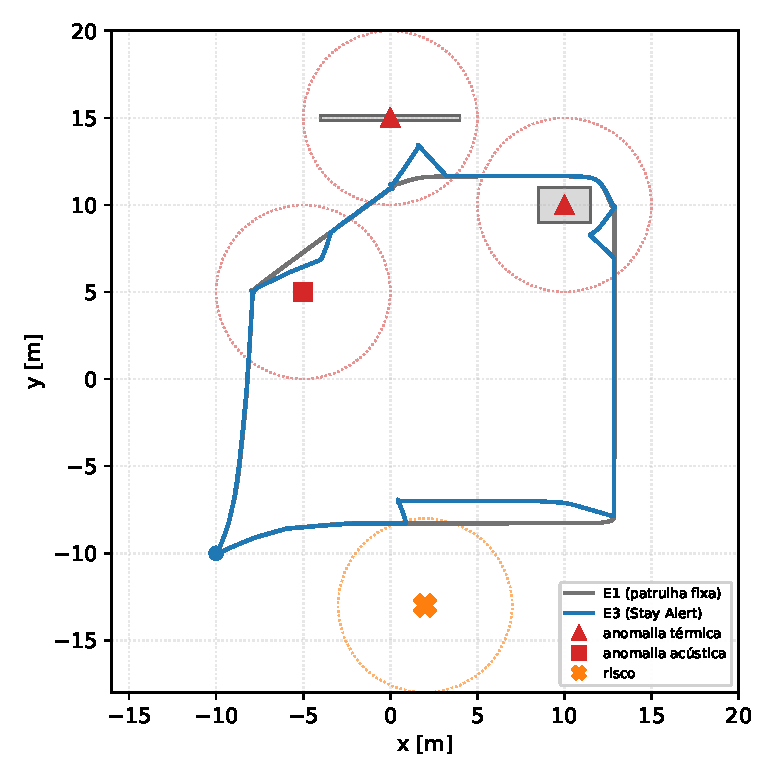
\includegraphics[width=0.85\textwidth]{figuras/traj_overlay}
\caption{Sobreposição de trajetórias da patrulha fixa (E1) e da camada reativa (E3)
no cenário padrão. A camada reativa abandona a perna de patrulha para alcançar a
pose de parada de cada anomalia e retorna à ronda; a patrulha fixa percorre o
circuito sem desvio.}
\label{fig:res-traj}
\end{figure}

\begin{figure}[htb]
\centering
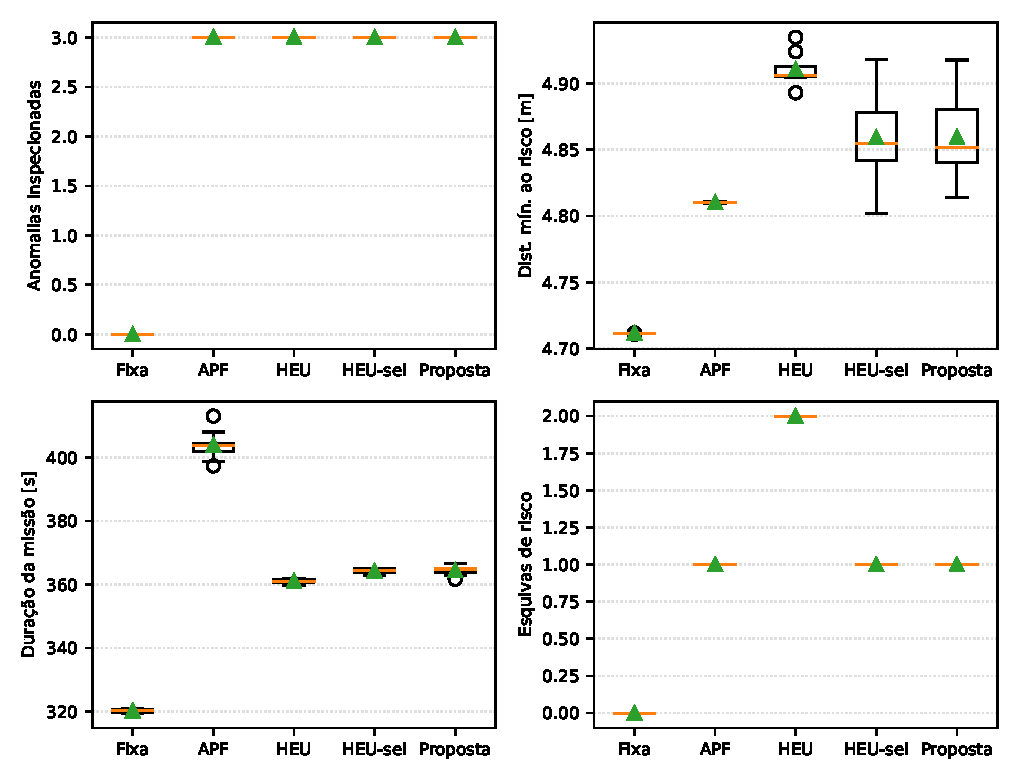
\includegraphics[width=0.95\textwidth]{figuras/box_panel}
\caption{Distribuições por execução das métricas principais ($\triangle$ = média),
todas no cenário \texttt{default}: a patrulha fixa, a linha de base de campo
potencial (APF), o supervisor heurístico genérico (HEU), a variante de seleção de um
fator (HEU-sel) e a camada proposta. A patrulha fixa nunca inspeciona nem recua; as
quatro configurações reativas inspecionam as três anomalias, e nenhuma diferença
estatisticamente detectável foi encontrada entre HEU-sel e a camada proposta em
qualquer das métricas exibidas. O HEU executa um segundo recuo e o APF precisa de
missão mais longa para as mesmas inspeções.}
\label{fig:res-box}
\end{figure}

\section{Isolando o Campo do Ato de Desviar}
\label{sec:res-heu}

As comparações da seção anterior contrastam a camada reativa com linhas de base que
ou não podem desviar (a patrulha fixa) ou alteram o controlador além do supervisor
(a linha de base de campo potencial). Nenhuma delas isola o \emph{campo} do ato de
desviar. Acrescentam-se, portanto, duas configurações que rodam sobre o \emph{mesmo}
controlador Nav2/MPPI, com a mesma percepção, o mesmo \textit{keep-out}, as mesmas
poses de aproximação, o mesmo critério de confirmação e a mesma lógica de retorno à
patrulha:

\begin{itemize}
    \item \textbf{HEU}, um supervisor genérico de
    detectar--selecionar--desviar--retornar: é acionado por \emph{detecção bruta}
    (um evento dentro do raio de sensoriamento) em vez de por limiar sobre $\Phi$,
    seleciona o alvo \emph{mais próximo} em vez do mais saliente, e arbitra pela
    regra simples ``risco no alcance $\Rightarrow$ desviar''. Substitui, portanto,
    tanto a ponderação por saliência quanto a arbitragem baseada em campo por
    equivalentes de detecção bruta. Note-se que ele ainda resolve riscos primeiro
    --- a verificação de preempção precede a verificação de atração ---, de modo que
    o que lhe falta não é uma regra de precedência, mas a persistência temporal que
    o campo com decaimento fornece.
    \item \textbf{HEU-sel}, variante de um fator: idêntica à camada proposta
    \emph{exceto} por selecionar o alvo mais próximo em vez do mais saliente.
\end{itemize}

Mudar o alvo selecionado não altera $\Phi$ no instante do disparo: o simulador
publica a intensidade de todo evento no alcance e o campo retém o máximo, de modo que
o cruzamento do limiar é o mesmo nos dois modos. Muda, porém, qual anomalia é
comprometida, e uma anomalia comprometida deixa de alimentar o campo. O contraste é,
assim, de seleção no ponto de decisão \emph{com} efeito a jusante sobre a evolução
temporal de $\Phi$, e não um mero reordenamento de atendimento.

A Tabela~\ref{tab:res-heu} relata os três cenários.

\paragraph*{Comparação primária (corrigida por Holm), cenário \texttt{default}.}
O HEU-sel não apresentou diferença estatisticamente detectável em relação à camada
proposta em nenhum dos cinco desfechos relatados ($p_{\mathrm{Holm}}=1{,}0000$ em
todos; $|\delta|\le0{,}19$; todos os intervalos \textit{bootstrap} contêm zero).
Dois dos cinco --- anomalias inspecionadas e recuos --- são constantes e idênticos
nos dois braços, enquanto os outros três variam. Trata-se de ausência de diferença
detectada com $n=10$, e não de demonstração de equivalência. Em contraste, o HEU
difere em recuos ($1$ contra $2$, $p_{\mathrm{Holm}}=3{,}0\times10^{-4}$), tempo de
investigação ($35{,}1$ contra $41{,}2$~s, $p_{\mathrm{Holm}}=0{,}0027$) e duração da
missão ($p_{\mathrm{Holm}}=0{,}0052$). A diferença de afastamento nesse cenário não
sobrevive à correção ($p_{\mathrm{Holm}}=0{,}0511$) e corresponde a $6$~cm, lida
aqui como operacionalmente irrelevante e relatada como tal, não como vantagem.

\paragraph*{Exploratório, cenário \texttt{conflict}.}
Nesse cenário um risco é colocalizado com uma anomalia \emph{mais saliente}, de modo
que as duas regras discordam por construção. A diferença é grande e na direção que a
precedência \emph{persistente} da camada proposta visa evitar: o HEU também
preempta, mas não mantém o canal de risco aberto. O HEU inspeciona a anomalia
colocalizada (mediana $4$ de $4$ contra $3$ da camada proposta) e paga por isso: o
afastamento mínimo cai de $4{,}84$ para $2{,}23$~m ($\delta$ de Cliff $+1{,}00$,
separação completa; IC \textit{bootstrap} da diferença $[+2{,}60;+2{,}63]$~m;
$p<0{,}0001$), os recuos sobem de $1$ para $4$ conforme o supervisor oscila, a
duração da missão cresce cerca de $106$~s, e o tempo até inspecionar o alvo
prioritário atrasa cerca de $105$~s em ambas as modalidades ($345{,}0$ contra
$239{,}9$~s na térmica; $387{,}6$ contra $283{,}1$~s na acústica). Para o HEU-sel,
novamente, nenhuma diferença em relação à camada proposta foi detectada em qualquer
desfecho relatado.

\paragraph*{Exploratório, cenário \texttt{adverse}.}
As três configurações alcançaram mediana de cinco anomalias inspecionadas, com
contagens por execução entre quatro e cinco (proposta $9/10$ execuções com cinco,
HEU $10/10$, HEU-sel $8/10$). O HEU executa um recuo adicional e as diferenças de
afastamento são da ordem de centímetros.

\begin{table}[htb]
\centering
\caption{Camada proposta contra supervisor genérico de
detectar--selecionar--desviar--retornar (HEU) e contra variante de seleção de um
fator (HEU-sel), todos sobre o mesmo controlador Nav2/MPPI. Medianas sobre execuções
válidas. O bloco \texttt{default} pertence à família de comparação primária
(corrigida por Holm); os blocos \texttt{conflict} e \texttt{adverse} são
exploratórios e são relatados com $p$ não corrigido. $n$: \texttt{default}
$10/9/10$, \texttt{conflict} $10/9/10$, \texttt{adverse} $10/10/10$
(proposta/HEU/HEU-sel).}
\label{tab:res-heu}
\footnotesize
\setlength{\tabcolsep}{4pt}
\begin{tabular}{llccccc}
\hline
\textbf{Cenário} & \textbf{Métrica} & \textbf{Proposta} & \textbf{HEU} &
\textbf{HEU-sel} & \textbf{$\delta$ (vs.\ HEU)} & \textbf{$p$ (vs.\ HEU)}\\
\hline
\texttt{default} & Anomalias inspecionadas    & $3$     & $3$     & $3$     & $+0{,}00$ & $1{,}0000^{\dagger}$\\
                 & Recuos                     & $1$     & $2$     & $1$     & $-1{,}00$ & $3{,}0\times10^{-4\dagger}$\\
                 & Dist.\ mín.\ ao risco [m]  & $4{,}85$  & $4{,}91$  & $4{,}85$  & $-0{,}73$ & $0{,}0511^{\dagger}$\\
                 & Tempo de investigação [s]  & $35{,}1$  & $41{,}2$  & $35{,}3$  & $-1{,}00$ & $0{,}0027^{\dagger}$\\
\hline
\texttt{conflict} & Anomalias inspecionadas   & $3$     & $4$     & $3$     & $-0{,}67$ & $0{,}0160$\\
                 & Recuos                     & $1$     & $4$     & $1$     & $-1{,}00$ & $0{,}0003$\\
                 & \textbf{Dist.\ mín.\ risco [m]} & $\mathbf{4{,}84}$ & $\mathbf{2{,}23}$ & $4{,}82$ & $+1{,}00$ & $<\!0{,}0001$\\
                 & Duração da missão [s]      & $363{,}7$ & $469{,}7$ & $364{,}4$ & $-0{,}89$ & $0{,}0013$\\
                 & Tempo até alvo prioritário [s]& $239{,}9$ & $345{,}0$ & $240{,}4$ & ---     & ---\\
\hline
\texttt{adverse} & Anomalias inspecionadas    & $5$     & $5$     & $5$     & $-0{,}10$ & $0{,}7337$\\
                 & Recuos                     & $1$     & $2$     & $1$     & $-1{,}00$ & $0{,}0002$\\
                 & Dist.\ mín.\ ao risco [m]  & $4{,}88$  & $4{,}90$  & $4{,}85$  & $-0{,}58$ & $0{,}0288$\\
\hline
\end{tabular}

\vspace{2pt}
\footnotesize $^{\dagger}$Corrigido por Holm dentro da família primária de $15$
testes. Linhas sem o símbolo são exploratórias e não corrigidas.
\end{table}

\subsection{O Que Se Pode e o Que Não Se Pode Atribuir}

Duas leituras decorrem desses números, e convém limitar cada uma.

Primeiro, o critério de \emph{seleção} não teve efeito detectável: nos cenários
\texttt{default} e \texttt{conflict} a camada proposta e o HEU-sel produziram o mesmo
valor constante em todo desfecho discreto ao longo das dez execuções de cada, e em
\texttt{adverse} os desfechos variam dentro dos dois grupos e se sobrepõem. Não se
alega equivalência --- com dez execuções por grupo, a falha em detectar uma diferença
não estabelece sua ausência, e não foram especificadas margens de equivalência para
essas métricas ---, apenas que o critério não fez diferença que aqui se pudesse
detectar.

Segundo, o efeito no cenário de conflito se prende ao \emph{modo de disparo}, por ser
este o único fator que separa HEU de HEU-sel. É preciso ser explícito quanto ao que
essa chave agrupa: ela substitui um limiar sobre o campo com decaimento por detecção
bruta instantânea, mudando o disparo \emph{e} removendo da decisão a persistência
temporal do campo. Ela \emph{não} remove a precedência de segurança. Os \textit{logs}
mostram o HEU preemptando a investigação três vezes por execução
(\texttt{deferred\_hazard}); cada adiamento libera o alvo, a atração volta a disparar
assim que o risco sai momentaneamente do alcance, e a inspeção acaba por se completar
--- o que é a oscilação visível como quatro recuos. Lê-se o efeito, portanto, como
perda de \emph{persistência temporal} no canal de risco, e não como ausência de regra
de precedência; apresenta-se essa como a leitura mais consistente com os
\textit{logs}, e não como fator isolado: separar a fonte do disparo da persistência
exigiria uma variante adicional que não foi executada.

\section{Resposta a Risco e Segurança}
\label{sec:res-seguranca}

A linha de base fixa registra zero esquivas de risco, enquanto a camada reativa
executa exatamente um recuo por encontro ($1{,}0\pm0{,}0$).

\subsection{Risco ao Lado da Rota}

Para o risco posicionado \emph{ao lado} da rota (E0--E5), o afastamento mínimo é
pequeno em termos absolutos para ambos, mas a camada reativa mantém afastamento
ligeiramente \emph{maior} e altamente consistente (E3, $4{,}86\pm0{,}03$~m) que a
linha de base fixa ($4{,}71\pm0{,}00$~m): a repulsão regula a aproximação a uma faixa
estreita, e a linha de base --- uma vez separadas as execuções com falha de partida
--- passa pelo risco lateral a uma distância fixa e marginalmente menor.

\subsection{Risco Sobre a Rota}

O teste mais informativo coloca o risco \emph{sobre} uma perna da patrulha
(configurações RHM, o método, e RHB, a linha de base fixa). Ali, a linha de base fixa
atravessa em linha reta, atingindo afastamento mínimo de apenas $0{,}71\pm0{,}00$~m
sem qualquer recuo e com tempo mínimo até a colisão de $2{,}8\pm0{,}1$~s. A camada
reativa produz resposta em duas escalas de tempo: tão logo o risco é detectado, ele é
projetado como zona de exclusão persistente no \textit{costmap} global --- de modo
que o planejador contorna pelo resto da missão --- e um recuo reativo rápido
($1{,}0\pm0{,}0$ evento de esquiva) trata a proximidade imediata. Os dois em conjunto
permitem ao robô contornar o risco a $1{,}71\pm0{,}01$~m (zero colisões nas execuções
válidas) com margem de tempo até a colisão de $5{,}6\pm0{,}9$~s, ainda inspecionando
todas as três anomalias ($3{,}0\pm0{,}0$), ao custo de tempo de $372\pm1$~s
(Tabela~\ref{tab:res-seguranca}).

A camada reativa, portanto, mais do que dobra o afastamento ($+1{,}00$~m; $\delta$ de
Cliff igual a $1$, $p<10^{-4}$) e aproximadamente dobra a margem de tempo até a
colisão ($+2{,}8$~s; $p<10^{-4}$) da patrulha fixa no caso que a repulsão existe para
tratar.

\begin{table}[htb]
\centering
\caption{Risco sobre a rota: desfechos de segurança (média\,$\pm$\,desvio padrão
sobre execuções válidas). RHB é a linha de base fixa (atravessa em linha reta); RHM é
o método --- recuo reativo combinado a zona de exclusão persistente disparada por
detecção, que o planejador contorna. $n$ válido: RHB $10$, RHM $9$.}
\label{tab:res-seguranca}
\footnotesize
\begin{tabular}{lcc}
\hline
\textbf{Métrica} & \textbf{RHB (base)} & \textbf{RHM (método)}\\
\hline
Anomalias inspecionadas        & $0{,}0\pm0{,}0$   & $3{,}0\pm0{,}0$\\
Recuos                         & $0{,}0\pm0{,}0$   & $1{,}0\pm0{,}0$\\
Colisões                       & $0{,}0\pm0{,}0$   & $0{,}0\pm0{,}0$\\
Dist.\ mín.\ ao risco [m]      & $0{,}71\pm0{,}00$ & $1{,}71\pm0{,}01$\\
Tempo mín.\ até colisão [s]    & $2{,}8\pm0{,}1$   & $5{,}6\pm0{,}9$\\
Tempo abaixo do afastamento [s]& $14{,}4\pm0{,}0$  & $9{,}2\pm0{,}1$\\
Duração da missão [s]          & $320\pm1$         & $372\pm1$\\
\hline
\end{tabular}
\end{table}

\subsection{A Quem Atribuir o Ganho de Segurança}
\label{sec:res-ablacao}

Para atribuir esse ganho a seus dois mecanismos, ablacionam-se ambos
(Tabela~\ref{tab:res-ablacao}). Com a \emph{zona de exclusão apenas} (KOa, recuo
reativo desabilitado) o planejador ainda contorna o risco e inspeciona as três
anomalias no mesmo afastamento de $1{,}71$~m, ligeiramente mais rápido que o método
completo ($352$ contra $372$~s). Com o \emph{recuo reativo apenas} (KOb, zona de
exclusão desabilitada) o robô não consegue livrar o risco sobre a rota: oscila
($29{,}6\pm3{,}9$ recuos), quase nada inspeciona ($0{,}2\pm0{,}4$) e estoura o tempo
($627\pm6$~s).

Essas duas ablações, porém, ainda carregam a camada reativa. A referência mais justa
é uma \emph{patrulha fixa portando a mesma zona de exclusão disparada por detecção e
nenhuma camada reativa}, que isola o \textit{keep-out} da ponderação; acrescenta-se,
portanto, a configuração KOF (camada reativa desabilitada, \textit{keep-out} ativo).
O KOF atinge afastamento mínimo mediano de $1{,}73$~m contra $1{,}71$~m da ablação
somente-\textit{keep-out} KOa --- diferença de $2$~cm que não é distinguível
($p_{\mathrm{Holm}}=0{,}4194$) --- e passa $9{,}0$~s abaixo da faixa de $2$~m contra
$9{,}3$~s.

\textbf{Atribui-se, portanto, o benefício de segurança sobre um risco na rota à zona
de exclusão disparada por detecção, e não à ponderação reativa.} O KOF não é cego ao
risco: ele percebe o risco e projeta a zona de exclusão; o que lhe falta é o
supervisor reativo.

O que a camada reativa acrescenta sobre o KOF é o comportamento de inspeção, e apenas
isso: o KOF inspeciona $0$ das $3$ anomalias em toda execução --- por construção,
pois sem camada reativa nenhuma investigação é jamais disparada --- contra $3$ de $3$
do KOa ($p_{\mathrm{Holm}}=1{,}6\times10^{-4}$), e completa a missão $31$~s mais
rápido ($320{,}9$ contra $352{,}2$~s, $p_{\mathrm{Holm}}=0{,}0021$) precisamente
porque nunca se desvia. O par KOF/KOa é, assim, uma decomposição e não uma vitória: a
zona de exclusão compra o afastamento, a camada reativa compra as inspeções, e as
duas coisas são separáveis.

A zona de exclusão deliberativa é, portanto, o mecanismo que resolve um risco sobre a
rota; o recuo reativo não acrescenta benefício mensurável para esse risco
\emph{estático}. Não se alega que o recuo ajude aqui --- seu valor aparece quando um
risco \emph{emerge} durante uma investigação, o que se quantifica a seguir.

\begin{table}[htb]
\centering
\caption{Ablação de zona de exclusão e recuo no risco sobre a rota
(média\,$\pm$\,desvio padrão sobre execuções válidas; $n=9$ para RHM, $10$ para KOa,
$9$ para KOb). RHM é o método completo (recuo $+$ zona de exclusão); KOa é
somente-zona (recuo desabilitado); KOb é somente-recuo (zona desabilitada).}
\label{tab:res-ablacao}
\footnotesize
\setlength{\tabcolsep}{5pt}
\begin{tabular}{lccc}
\hline
\textbf{Métrica} & \textbf{RHM} & \textbf{KOa} & \textbf{KOb}\\
 & \textbf{(recuo+zona)} & \textbf{(zona)} & \textbf{(recuo)}\\
\hline
Anomalias inspecionadas     & $3{,}0\pm0{,}0$   & $3{,}0\pm0{,}0$   & $0{,}2\pm0{,}4$\\
Recuos                      & $1{,}0\pm0{,}0$   & $0{,}0\pm0{,}0$   & $29{,}6\pm3{,}9$\\
Colisões                    & $0{,}0\pm0{,}0$   & $0{,}0\pm0{,}0$   & $0{,}0\pm0{,}0$\\
Dist.\ mín.\ ao risco [m]   & $1{,}71\pm0{,}01$ & $1{,}71\pm0{,}01$ & $4{,}29\pm0{,}08$\\
Tempo mín.\ até colisão [s] & $5{,}6\pm0{,}9$   & $5{,}8\pm0{,}1$   & $8{,}7\pm0{,}2$\\
Duração da missão [s]       & $372\pm1$         & $352\pm1$         & $627\pm6$\\
\hline
\end{tabular}
\end{table}

\section{O Valor do Recuo Diante de Risco Emergente}
\label{sec:res-emergente}

A ablação anterior mostra que, para um risco \emph{estático} sobre a rota, a zona de
exclusão deliberativa sozinha (KOa) iguala o método completo e o recuo reativo não
acrescenta benefício mensurável. O recuo foi projetado, contudo, para um risco que
\emph{emerge} enquanto o robô já está comprometido com uma inspeção --- o caso para o
qual a preempção do Algoritmo~\ref{alg:stayalert} foi construída e que os cenários
estáticos não conseguem exercitar.

Testa-se isso diretamente (configurações DHa, DHb): um risco colocalizado com uma
anomalia permanece inativo --- não publicado nem ao canal reativo nem à zona de
exclusão deliberativa --- até que o robô, já investigando, se aproxime a $3$~m, ponto
em que o ambiente o ativa. O instante de ativação e a primeira publicação em cada
canal são registrados por execução.

Os valores de afastamento e de tempo radial até a colisão abaixo são mínimos
\emph{de missão inteira} relativos à localização do risco, incluindo o período
anterior à ativação: o coletor não reinicia essas métricas na ativação. Esses
resultados comparam, portanto, margens de nível de missão no cenário de risco
emergente, e não estimam efeito de TTC pós-ativação separado. O tempo de simulação
preservado na auditoria permite localizar o mínimo de \emph{distância}: ele é
atingido após a ativação em todas as $18$ execuções dinâmicas válidas. Não se estende
isso ao mínimo de TTC --- que, sendo uma razão envolvendo velocidade radial, pode já
carregar valor anterior à ativação ---, de modo que a diferença de TTC é relatada
estritamente como margem de missão inteira.

Com o recuo reativo ativo (DHa) a preempção dispara em \emph{toda execução válida}
($8/8$ investigações adiadas) e o robô se afasta, mantendo afastamento mínimo de
$2{,}55\pm0{,}15$~m e tempo radial até a colisão de $5{,}23\pm0{,}45$~s. Com o recuo
desabilitado (DHb, somente zona de exclusão) o robô prossegue até a pose de parada da
inspeção, aproximando-se a $2{,}22\pm0{,}01$~m ($4{,}72\pm0{,}21$~s).

O recuo reativo compra, portanto, $+0{,}33$~m de afastamento (IC $95\%$
$[+0{,}23;+0{,}42]$, $\delta$ de Cliff igual a $1$, $p=4{,}6\times10^{-5}$) e
$+0{,}51$~s de margem de tempo até a colisão ($[+0{,}20;+0{,}84]$, $\delta=0{,}85$,
$p=1{,}0\times10^{-3}$) contra um risco emergente.

Essa margem é uma troca deliberada, não um ganho gratuito: DHa roda cerca de
$9{,}4$~s a mais ($348$ contra $338$~s) e $1{,}6$~m a mais, e \emph{adia} a inspeção
agora arriscada (DHa não inspeciona o alvo em execução alguma; DHb o inspeciona em
todas), comprando margem de segurança maior naquele encontro ao preço de uma inspeção
completada. Nenhuma das configurações entra na região de contato, e nenhuma passa
tempo algum abaixo do limiar de afastamento de $2$~m, de modo que o efeito é
diferença de \emph{margem}, não de contatos observados.

Distingue-se ainda o disparo da preempção de um recuo limpamente completado: em $3$
das $8$ execuções válidas de DHa, a meta de navegação do recuo é ela própria
abortada, e ainda assim cada episódio termina como esquiva bem-sucedida --- o campo
decai abaixo do limiar uma vez que o risco é entregue à zona de exclusão (saída
\emph{segura}) --- e o afastamento relatado é o mínimo de \emph{posição verdadeira}
do coletor de métricas, não uma chegada presumida à pose de recuo (essas três
execuções mantêm, de fato, $2{,}70$~m). A contribuição do recuo é, assim, uma margem
de segurança \emph{transiente} quando um risco aparece no meio da investigação ---
benefício que a ablação estática sobre a rota, por construção, não pode revelar.

\section{Precedência de Segurança sob Conflito}
\label{sec:res-conflito}

Os cenários precedentes separam atração e repulsão no espaço, de modo que o campo
nunca precisa arbitrar entre uma anomalia e um risco no mesmo local. O cenário de
conflito (CONF) força exatamente essa decisão: uma anomalia acústica \emph{forte}
($|w\,I_e|=1{,}14$) é colocalizada com um risco \emph{mais fraco}
($|w\,I_e|=1{,}05$) em $(2,-13)$, de sorte que uma regra de seleção puramente por
magnitude --- que retém o sinal mais saliente --- preferiria inspecionar a anomalia e
jamais disparar um recuo. A regra de precedência resolve primeiro qualquer risco
acima do limiar, independentemente de uma atração concorrente mais forte.

Trata-se de propriedade categórica de \emph{seleção}, não de efeito médio, e por isso
é relatada como frequência de desfecho e não como comparação de médias. Nas dez
execuções de CONF (todas válidas), o comportamento foi idêntico em todas:
\textsc{Avoid} foi disparado ($10/10$ execuções, $1{,}0\pm0{,}0$ recuos) e a anomalia
forte colocalizada \emph{nunca} foi inspecionada, de modo que o robô inspecionou
apenas as três anomalias fora do conflito ($3{,}0\pm0{,}0$). O robô manteve
afastamento mínimo ao risco de $4{,}84\pm0{,}02$~m e tempo mínimo até a colisão de
$17{,}3\pm1{,}6$~s, com \emph{zero} colisões em todas as execuções, a uma duração de
missão ($364\pm2$~s) indistinguível da do cenário padrão.

O campo reativo impõe, portanto, uma \emph{prioridade de seleção com risco em
primeiro lugar} por construção, confirmada empiricamente no único caso projetado para
quebrar uma interpretação puramente de magnitude. Essa é uma escolha deliberada de
projeto --- a prioridade é \emph{rígida}, de modo que um risco pouco acima do limiar
(um possível falso positivo) suprime mesmo uma anomalia genuína fortemente saliente
--- e aceita-se o risco resultante de excesso de conservadorismo. Distingue-se essa
prioridade \emph{lógica} de uma garantia física de segurança: ela vale sob condições
explícitas (uma pose de recuo disponível e fora da janela refratária pós-recuo), e o
cenário estático CONF não exercita casos como o de um segundo risco surgindo durante
a janela refratária. O que se relata como desfecho de \emph{segurança} é o
afastamento observado e a ausência de entradas na região de contato, não uma garantia
de invariância.

\section{O Custo da Precedência e Sua Sensibilidade}
\label{sec:res-custo-precedencia}

A seção anterior aceita um risco de excesso de conservadorismo próximo ao limiar sem
medi-lo. Mede-se agora, e sonda-se separadamente se o limiar que governa a
precedência está bem posicionado. Ambas as análises são exploratórias.

\subsection{Um Risco Marginalmente Elegível Custa Uma Inspeção, Deterministicamente}

O canal de risco tem memória: uma observação eleva $h$, e $h$ decai então por
$\lambda$ a cada período até cair abaixo de $\varepsilon$. Como o limiar de
modalidade é aplicado à intensidade bruta percebida, o risco elegível \emph{mais
fraco} já produz $h=|w_{\mathcal{H}}|\,\theta_{\mathcal{H}}$, que aqui iguala o
limiar de entrada do supervisor; um recuo dispara, portanto, uma vez, no pico. Após
um único passo de decaimento, porém, $h$ está abaixo do limiar de entrada enquanto
ainda acima de $\varepsilon$ --- de modo que o risco continua \emph{governando} o
campo, e assim continua suprimindo qualquer atração, sem disparar recuo adicional.

Construiu-se a configuração CM para exercitar exatamente essa faixa: um risco de
intensidade elegível mínima ao lado da primeira perna de patrulha, que o robô observa
e então deixa para trás, junto a uma anomalia acústica legítima de intensidade
$0{,}95$ --- o evento mais saliente do cenário --- posicionada a $4{,}3$~m do risco,
bem fora dele.

O resultado é o mesmo nas dez execuções: exatamente um recuo dispara e a anomalia
saliente \emph{nunca} é inspecionada ($0/10$), de modo que o robô encerra toda missão
tendo inspecionado $3$ das $4$ anomalias, abrindo mão da mais forte. Define-se a
janela de supressão como o intervalo entre a primeira e a última amostra registrada
em que o canal de risco governa o campo ($\Phi<0$) enquanto sua magnitude está abaixo
do limiar de recuo. Assim medida, ela dura $69{,}5$~s (faixa $67{,}3$--$72{,}4$). Não
é puro decaimento: o risco é reobservado dentro da janela e a magnitude do campo
volta a subir em uma mediana de duas amostras por execução, razão pela qual ela
excede os cerca de $39$~s que o decaimento sozinho, a partir da magnitude inicial,
daria.

A precedência categórica, portanto, não apenas arrisca excesso de conservadorismo:
nessa configuração ela custa uma inspeção em toda execução. O custo é incorrido sob
condições em que a própria camada não agiria sobre o risco --- ao longo de toda a
janela a distância mínima do robô a ele é de $3{,}92$~m (faixa $3{,}86$--$4{,}06$) e
sua magnitude está abaixo do limiar de recuo.

Enfatiza-se uma leitura que os números \emph{não} sustentam. CM e o cenário de
conflito completo terminam ambos com três anomalias inspecionadas, mas os dois trêses
não são comparáveis: em CONF a anomalia preterida é colocalizada com o risco e
\emph{deve} ser recusada, ao passo que em CM ela é alvo legítimo a $4{,}3$~m de
distância. A mesma contagem é comportamento correto em um cenário e falha no outro.

\subsection{Sensibilidade Local ao Limiar de Elegibilidade do Risco}

Variar o limiar de entrada do supervisor não testa a precedência, porque o que
governa a supressão é o limiar de \emph{elegibilidade de modalidade}
$\theta_{\mathcal{H}}$, aplicado antes da ponderação. Varre-se esse limiar sobre
$\{0{,}20;\,0{,}30;\,0{,}40\}$ no cenário de conflito, com $0{,}30$ o valor usado ao
longo de todo o trabalho.

Baixá-lo para $0{,}20$ não produziu diferença estatisticamente detectável
(afastamento $4{,}85$ contra $4{,}83$~m, $p=0{,}39$; inspeções e recuos idênticos).
Elevá-lo para $0{,}40$ \emph{degrada} a segurança: o afastamento mínimo cai para
$3{,}78$~m ($\delta$ de Cliff $+1{,}00$, IC \textit{bootstrap} da diferença
$[+0{,}99;+1{,}10]$~m, $p<0{,}0001$) e a missão se alonga em $9{,}1$~s, porque limiar
de elegibilidade mais alto significa que o risco é reconhecido mais tarde e, portanto,
mais perto. Relatam-se esses dois contrastes sem inferir curva de resposta geral a
partir de três valores; o que eles estabelecem é que o afastamento relatado no
restante do trabalho não é produzido por um limiar escolhido abaixo do valor em que a
degradação aparece.

\subsection{Histerese: Sem Efeito Detectável da Largura Testada, mas a Posição Importa}

Comparam-se três pares de entrada/saída escolhidos de modo que posição e largura
variem independentemente: a referência $(0{,}45;\,0{,}25)$, de largura $0{,}20$; uma
faixa mais estreita $(0{,}45;\,0{,}35)$, de largura $0{,}10$ no mesmo ponto de
entrada; e uma faixa deslocada $(0{,}55;\,0{,}35)$, de mesma largura $0{,}20$.

Reduzir a largura à metade não produziu diferença estatisticamente detectável em
qualquer desfecho relatado: desvios de rota, inspeções, duração da missão e tempo de
investigação dão todos $p\ge0{,}60$ contra a referência, com intervalos
\textit{bootstrap} contendo zero.

Deslocar o ponto de entrada dobra os desvios de rota contabilizados (mediana
$4\rightarrow8$, $\delta=-1{,}00$, $p=0{,}0003$) e reduz o tempo \emph{total} por
execução em \textsc{Investigate} (mediana $35{,}1\rightarrow26{,}6$~s, $p=0{,}0003$),
mantendo inalteradas as inspeções creditadas em $3$ de $3$. Mais desvios e menos
tempo total de investigação são, em conjunto, consistentes com o robô se comprometer
mais perto de cada alvo uma vez que o limiar de entrada é mais alto, mas os dois
agregados não separam duração de episódio de contagem de episódios, e não se
instrumentaram durações por episódio; oferece-se essa leitura como interpretação, e
não como medida. A métrica de desvios de rota deve ser lida como sensível à
\emph{posição} do limiar de entrada, e não como contagem intrínseca do cenário.

\section{Custo do Comportamento de Inspeção}
\label{sec:res-custo}

O comportamento acrescentado é barato: a duração de missão de E3 ($364\pm1$~s) é
aumento modesto sobre a linha de base fixa ($320\pm0$~s) pelos desvios de inspeção
($+6{,}2$~m percorridos). Enquadrado como troca de utilidade, cada anomalia adicional
inspecionada custa cerca de $2$~m de percurso extra ($+6{,}2$~m para três) e $15$~s
de tempo de missão ($+44$~s para três) --- troca favorável, dado que a linha de base
fixa não inspeciona \emph{nenhuma}.

\subsection{Lendo o Custo contra a Ronda}

Expresso contra a ronda que estende, o comportamento custa $14\%$ da duração da
patrulha: $320\pm0$~s tornam-se $364\pm1$~s por três inspeções. A maior parte desse
incremento é explicada pelo tempo total por execução em \textsc{Investigate} (mediana
$35{,}1$~s sobre os três episódios) e, como a permanência comandada é de apenas
$t_{\text{dwell}}=3$~s por episódio, o custo é dominado pelo desvio até a pose de
parada, e não pela pausa de inspeção em si.

Ele é também incorrido por \emph{evento}, e não por metro patrulhado, de modo que uma
ronda mais longa carregando o mesmo número de eventos distribuiria os mesmos segundos
absolutos sobre uma base maior e a penalidade relativa cairia. O cenário denso custa
mais em termos absolutos ($397\pm4$~s para $4{,}9\pm0{,}3$ inspeções) porque apresenta
mais eventos; seu \textit{layout} difere do padrão, de modo que não se lê a diferença
entre as duas rondas como incremento controlado.

A leitura prática para um operador é que cada inspeção creditada custa cerca de
$15$~s de tempo de ronda e cerca de $2$~m de percurso, e que uma ronda planejada com
essa folga para o número esperado de eventos absorve o comportamento sem
reprogramação da patrulha --- com a ressalva, da Seção~\ref{sec:res-ruido}, de que os
eventos precisam primeiro ser detectados.

\subsection{Comparação com a Linha de Base de Campo Potencial}

A camada proposta completa as mesmas três inspeções mais rápido ($364$ contra
$404\pm5$~s) sobre comprimento de caminho essencialmente igual ($86{,}6$ contra
$86{,}4$~m, diferença de $0{,}2$~m que não se lê como vantagem em direção alguma).

É preciso ser explícito quanto ao que essa comparação \emph{não} isola: a linha de
base APF substitui o supervisor reativo \emph{e} o controlador --- ela comanda
velocidades diretamente, em vez de emitir metas ao Nav2/MPPI ---, de modo que a
diferença confunde supervisor com controlador. Quanto ao ajuste, declaram-se
procedimento e valores. Os ganhos do APF foram calibrados para que a linha de base
dispare dentro do mesmo raio de sensoriamento da camada proposta --- atração cruzando
seu limiar em cerca de $4$ a $5$~m para \textit{waypoints} e repulsão na passagem a
cerca de $4{,}7$~m do risco lateral ---, critério de comparabilidade que foi o
aplicado. Os valores resultantes são $k_{\text{att}}=1{,}5$, $k_{\text{rep}}=4{,}0$,
$k_{\text{obs}}=0{,}6$, limiares de disparo e de saída de $0{,}15$ e $0{,}08$ sobre a
magnitude da força, e período refratário pós-recuo de $12$~s, acrescentado contra a
oscilação que a formulação de campo potencial exibe quando uma perna de patrulha
passa dentro da região de disparo. Além da calibração de alcance de disparo não se
buscou mais sobre esses valores, e a vantagem de tempo deve ser lida com isso em
mente. A comparação que \emph{de fato} isola o supervisor, sobre controlador e
parâmetros compartilhados, é a heurística da Seção~\ref{sec:res-heu}.

\section{Cenário Adverso}
\label{sec:res-adverso}

No cenário denso em eventos (E5) o robô arbitra entre eventos aglomerados pela regra
de precedência, inspecionando em média $4{,}9\pm0{,}3$ das cinco anomalias, com
desvios correspondentemente mais numerosos ($9{,}4\pm0{,}8$) e missão mais longa
($397\pm4$~s). A inspeção completa das cinco é bem-sucedida em $9$ de $10$ execuções
(intervalo de Wilson de $95\%$ $[0{,}60;\,0{,}98]$).

A trilha de auditoria por episódio mostra a causa com precisão: todos os cinco alvos
são \emph{iniciados} em toda execução, e a incompletude é falha de navegação, não
falha em revisitar. Três execuções registraram falha de navegação reativa; duas delas
subsequentemente \emph{iniciaram uma investigação adicional} e completaram os cinco
alvos, enquanto a execução restante terminou com quatro inspeções creditadas e
\emph{nenhuma nova tentativa registrada} sobre o alvo falho. As duas investigações
adicionais são relatadas como observação dos episódios, não como demonstração de
política de nova tentativa: o ramo \texttt{failed} marca o alvo como falho mas não o
remove do conjunto comprometido, de modo que um início posterior é possível, mas não
garantido por regra explícita de recuperação.

Esse limite de densidade --- a navegação reativa ocasionalmente falhando sobre um
alvo densamente aglomerado --- é medido, e não suposto inexistente, sem entradas na
região de contato observadas. Não se alega escalabilidade geral a partir de uma única
configuração adversa, e varreduras mais amplas de densidade e geometria permanecem
trabalho futuro.

\section{Robustez a Ruído de Percepção}
\label{sec:res-ruido}

Como a abstração de eventos fornece modalidade, intensidade e posição sem incerteza,
sonda-se a sensibilidade do método a essa idealização injetando ruído gaussiano de
média zero sobre a posição e a intensidade percebidas do evento a cada ciclo de
sensoriamento.

Sob ruído moderado (posição $\sigma=0{,}3$~m, intensidade $\sigma=0{,}05$;
configuração N1) o método não é afetado: inspeciona todas as três anomalias em toda
execução válida ($3{,}0\pm0{,}0$), com a resposta a risco preservada e sem colisões.

Sob ruído alto ($\sigma=0{,}6$~m, $\sigma=0{,}10$; N2), a completude de inspeção se
degrada para $4/9$ inspeções completas, e os \textit{logs} permitem atribuir a causa
com precisão: as três anomalias ainda são \emph{detectadas} em toda execução, mas a
estimativa ruidosa de posição conduz o robô a um ponto a partir do qual o avaliador
não consegue confirmar a chegada à anomalia \emph{verdadeira}, de modo que $6$ das
$27$ inspeções comprometidas (ao longo das $9$ execuções válidas) são
\emph{rejeições na confirmação} --- e não esgotamentos de tempo ou abortos de
navegação, dos quais os arquivos CSV não registram nenhum. A inspeção completa
sucede, portanto, em $4$ de $9$ execuções válidas ($2{,}3\pm0{,}7$ anomalias;
intervalo de Wilson de $95\%$ $[0{,}19;\,0{,}73]$ para a taxa de conclusão por
missão).

Nenhuma entrada na região de contato foi observada, e o recuo diante do risco foi
preservado ($1{,}7\pm0{,}5$; Tabela~\ref{tab:res-ruido}); o afastamento mínimo médio
ao risco de fato \emph{aumentou}, de $4{,}86\pm0{,}03$~m em E3 para
$5{,}29\pm0{,}20$~m em N2. Esses resultados descrevem a troca observada sob os níveis
de ruído testados --- a completude de inspeção cai, pela etapa de confirmação,
enquanto nenhum contato é observado e o afastamento medido cresce --- e não
estabelecem garantia geral de segurança.

\begin{table}[htb]
\centering
\caption{Robustez a ruído de percepção (método, média\,$\pm$\,desvio padrão). E3 é
sem ruído; N1 e N2 adicionam ruído gaussiano de média zero, moderado e alto, sobre
posição ($\sigma_p$) e intensidade ($\sigma_i$) do evento. ``Taxa de inspeção
completa'' é a fração por missão de execuções que inspecionam todas as três
anomalias. $n$ válido: E3 $10$, N1 $10$, N2 $9$.}
\label{tab:res-ruido}
\footnotesize
\begin{tabular}{lccc}
\hline
\textbf{Métrica} & \textbf{E3 (sem)} &
\textbf{N1 ($\sigma_p{=}0{,}3$)} & \textbf{N2 ($\sigma_p{=}0{,}6$)}\\
\hline
Anomalias inspecionadas    & $3{,}0\pm0{,}0$  & $3{,}0\pm0{,}0$  & $2{,}3\pm0{,}7$\\
Taxa de inspeção completa  & $10/10$          & $10/10$          & $4/9$\\
Recuos                     & $1{,}0\pm0{,}0$  & $1{,}1\pm0{,}3$  & $1{,}7\pm0{,}5$\\
Colisões                   & $0{,}0\pm0{,}0$  & $0{,}0\pm0{,}0$  & $0{,}0\pm0{,}0$\\
Dist.\ mín.\ ao risco [m]  & $4{,}86\pm0{,}03$& $5{,}01\pm0{,}11$& $5{,}29\pm0{,}20$\\
Duração da missão [s]      & $364\pm1$        & $367\pm5$        & $374\pm8$\\
\hline
\end{tabular}
\end{table}

\section{Ameaças à Validade}
\label{sec:res-ameacas}

Esta seção enumera o que a avaliação não estabelece.

\paragraph*{Percepção idealizada.} A percepção é abstraída em eventos-oráculo. A
Seção~\ref{sec:res-ruido} relaxa parcialmente essa idealização, mas falsos positivos,
falsos negativos, persistência de eventos e erro de localização permanecem fora do
estudo. A transformada de localização é fixa.

\paragraph*{Apenas simulação.} Todos os resultados vêm do Gazebo Fortress. Não há
validação em subestação física, e não se alega transferência direta para
\textit{hardware}.

\paragraph*{Tamanho amostral.} Com $8$ a $10$ execuções válidas por configuração, a
ausência de diferença detectada não demonstra equivalência, e a ausência observada de
entradas na região de contato limita, mas não elimina, o risco. O limite superior
unilateral exato de $95\%$ sobre a probabilidade por execução de tal entrada,
$1-0{,}05^{1/n}$, é de $25{,}9\%$ para um grupo de $10$ execuções, $28{,}3\%$ para um
grupo de $9$ e $31{,}2\%$ para o grupo de $8$ execuções de DHa. Esse limite de risco é
consequência do tamanho amostral, não medida de desempenho.

\paragraph*{Desfechos retrospectivos.} Como registrado na
Seção~\ref{sec:res-familias}, os três contrastes primários precedem os dados, mas o
conjunto de cinco desfechos foi fixado após as execuções. A correção de Holm trata a
multiplicidade dentro da família relatada; ela não torna prospectiva a seleção de
desfechos.

\paragraph*{Generalização de cenário.} Cada propriedade comportamental foi
estabelecida em uma configuração projetada para exercitá-la. Um único cenário adverso
não estabelece escalabilidade a \textit{layouts} mais densos, e um único cenário de
conflito não estabelece a precedência sob toda geometria de conflito.


% ---
% Finaliza a parte no bookmark do PDF, para que se inicie o bookmark na raiz
% ---
\bookmarksetup{startatroot}% 
% ---

% ---
% Conclusão
% ---
\chapter{Conclusão}
\label{cap:conclusao}

Esta tese apresentou uma arquitetura de navegação em duas camadas para inspeção de
subestações elétricas: uma patrulha deliberativa de sensoriamento ativo conduz os
sensores até onde eventos possam ocorrer, e uma camada reativa produz um impulso de
aproximação acionado por limiar em direção a anomalias e um impulso de recuo diante
de riscos, a partir de um campo de atração/repulsão $\Phi$ derivado da saliência
sensorial e arbitrado por uma precedência categórica de segurança. A arquitetura
roda sobre uma pilha madura e reprodutível (ROS~2 $+$ Nav2/MPPI $+$ Gazebo Fortress).

\section{Síntese das Atribuições}
\label{sec:conc-atribuicoes}

A avaliação do Capítulo~\ref{cap:resultados} \emph{estreita} aquilo que pode ser
creditado à camada reativa. As três atribuições são enunciadas aqui sem rodeios,
porque a precisão quanto ao que cada mecanismo entrega é parte da contribuição.

\subsection{O Ganho de Segurança no Risco Estático Vem da Zona de Exclusão}

Sobre um risco \emph{estático} colocado na rota de patrulha, uma patrulha fixa
portando a mesma zona de exclusão disparada por detecção e nenhum supervisor reativo
(KOF) e a ablação somente-zona que retém a inspeção reativa (KOa) alcançaram
afastamentos mínimos medianos semelhantes ($1{,}73$ e $1{,}71$~m), sem diferença
estatisticamente detectável ($p_{\mathrm{Holm}}=0{,}4194$); o método completo (RHM)
situa-se nos mesmos $1{,}71$~m.

%% Delimitado em 13/11/2026. A atribuicao vale para o cenario e as configuracoes
%% estudadas; ausencia de beneficio adicional detectado nao demonstra equivalencia
%% geral entre os componentes.
Nesse cenário e nessas configurações, portanto, o benefício de segurança é atribuível
à zona de exclusão deliberativa, e não à ponderação reativa. A afirmação é dessa
extensão: ela não estabelece equivalência geral entre os dois componentes, nem se
transfere a riscos que não estejam estáticos sobre a rota: a comparação de risco
emergente da Seção~\ref{sec:res-emergente} mostra justamente o caso em que a resposta
reativa acrescenta margem. O que a camada reativa acrescenta sobre o KOF são as
inspeções em si ($3$ contra $0$ de $3$), ao custo de cerca de $31$~s de tempo de
missão adicional para o KOa.

\subsection{O Critério de Seleção Não Teve Efeito Detectável; o Modo de Disparo Teve}

Uma variante que difere apenas por selecionar o alvo mais próximo em vez do mais
saliente produziu os mesmos desfechos discretos constantes que a camada proposta ao
longo das dez execuções nos cenários \texttt{default} e \texttt{conflict}, e
distribuições sobrepostas em \texttt{adverse}. Não se alega equivalência: apenas
que nenhuma diferença foi detectada neste tamanho amostral.

O que \emph{mudou} o desfecho foi o \emph{modo de disparo}: uma heurística genérica
de detectar--selecionar--desviar--retornar, sobre o mesmo controlador Nav2/MPPI e
acionada por detecção bruta, acaba por inspecionar a anomalia colocalizada com um
risco e reduz o afastamento mínimo à metade ($4{,}84$ contra $2{,}23$~m, $\delta$ de
Cliff $-1{,}00$ na convenção comparador-menos-método adotada em toda a tese: o braço
comparado é o menor), ao mesmo tempo em que atrasa a inspeção prioritária em cerca de
$105$~s.

Essa troca \emph{não} remove a precedência categórica --- a heurística ainda
preempta, três vezes por execução ---, mas altera conjuntamente o sinal de decisão e
sua persistência temporal, de modo que os dois não são separáveis com as $32$
configurações da matriz principal. Os \textit{logs} de episódio são consistentes com
uma explicação ligada à persistência, e uma verificação posterior a sustenta em parte:
encurtar o período de decaimento \emph{mantendo fixa} a fonte do disparo encurta o
tempo em investigação com separação completa no braço que dispara sobre o campo, e não
separa nenhum desfecho no braço que dispara por detecção bruta
(§\ref{sec:res-relogio-consistente}).

%% CORRIGIDO em 16/11/2026. "Nao move desfecho algum" afirmava efeito nulo; o que houve
%% foi ausencia de separacao completa, com deltas pequenos e nao nulos, e sem teste de
%% equivalencia que autorizasse a leitura forte.
Não separar não é o mesmo que não mover: os deltas naquele braço são pequenos, não
nulos, e o protocolo não inclui teste de equivalência. A persistência, portanto, não é
inerte onde é consultada; sobre o braço que não a consulta, o que se tem é ausência de
separação detectada. Que fração do efeito no cenário de conflito lhe cabe permanece sem medida,
porque essa verificação encurta a persistência em vez de removê-la e correu no cenário
\texttt{default}.

\subsection{A Precedência Tem Custo Medido}

%% Delimitado em 15/11/2026. A frase anterior juntava num so enunciado a
%% janela de ~70 s e a inspecao perdida. Sob o relogio especificado a inspecao perdida
%% persiste (10/10 tambem) e a janela nao: o recuo que a abre deixa de disparar. Os
%% dois fatos foram separados porque tem estatutos diferentes.
Essa precedência carrega um custo que foi medido: um risco marginalmente elegível faz o
robô abrir mão de uma de quatro inspeções em $10/10$ execuções, e isso se repete nas
duas implementações temporais testadas: $20/20$ ao todo. A supressão da atração por
cerca de $70$~s que acompanha esse custo, e o recuo único que a abre, pertencem ao
relógio efetivamente executado: sob o período especificado o recuo não dispara
(§\ref{sec:res-relogio-consistente}). O que se repete nas duas implementações é o
\emph{desfecho}, três de quatro inspeções, e não a sua causa: sob o relógio especificado
duas das investigações terminaram por aborto de navegação
(§\ref{sec:res-relogio-consistente}), de modo que a mesma perda não é atribuída ao mesmo
mecanismo nos dois casos. Resultado repetido entre condições não identifica
mecanismo.

%% Delimitado em 13/11/2026. A frase anterior afirmava sem condicao que o
%% distintivo e o canal de risco "e nao a ponderacao por saliencia". A segunda
%% metade e ausencia de efeito DETECTADO nos cenarios e no tamanho amostral
%% executados, e nao demonstracao de que a ponderacao seja inutil.
Em conjunto, nos cenários executados e com oito a dez execuções por braço, o que
distingue esta camada de uma heurística genérica de desviar e retornar é o canal de
risco com limiar e decaimento. A ponderação por saliência, no mesmo conjunto de
condições, não produziu diferença detectável, o que delimita a sua contribuição
\emph{nestas distribuições de eventos} e não estabelece que ela seja dispensável em
outras, com anomalias de intensidades mais separadas ou em maior número. E a camada
troca completude por afastamento de um modo que está agora quantificado nas duas
direções.

\section{Limites da Evidência}
\label{sec:conc-limites}

%% Reescrito em 13/11/2026: os numeros da reavaliacao do limiar de
%% confirmacao apareciam aqui pela primeira vez, o que fazia da conclusao um capitulo
%% com resultado inedito. Eles passam a ser apresentados na
%% Secao~\ref{sec:res-confirmacao}, e aqui apenas se sintetiza.
A completude de inspeção é relatada como a taxa de execuções que inspecionam
\emph{todas} as anomalias: $10/10$ com percepção limpa, $4/9$ sob ruído alto de
percepção e $9/10$ sob aglomeração densa. Conforme a
Seção~\ref{sec:res-confirmacao}, essa taxa mistura dois efeitos que a análise separa e
que ambos existem: o critério de confirmação é sensível ao limiar adotado, e a
aproximação física também se degrada sob ruído. Elevar o limiar não corrige a segunda
coisa --- apenas deixa de contar a primeira ---, razão pela qual o critério adotado
permanece o justificado por construção.

Nenhuma entrada na região de contato de $0{,}5$~m foi observada em qualquer
configuração, mas com $8$ a $10$ execuções válidas por grupo o limite superior
unilateral exato de $95\%$ sobre a probabilidade por execução de tal entrada
permanece entre $25{,}9\%$ e $31{,}2\%$; e, sobre o risco na rota, o método transita
\emph{dentro} da faixa consultiva de afastamento de $2$~m que ele próprio relata, por
cerca de $9$~s por execução. Esses são os limites da evidência de segurança, e não
uma garantia de segurança.

\section{Escopo}
\label{sec:conc-escopo}

A avaliação é em simulação. A percepção é abstraída em eventos-oráculo, e não em
fluxos brutos de sensores, e a transformada de localização é mantida fixa. Os
resultados caracterizam, portanto, a \emph{lógica de decisão} da arquitetura e não
devem ser lidos como validação de um sistema de inspeção autônoma pronto para
implantação.

A região de contato de $0{,}5$~m e a faixa de afastamento de $2$~m são distâncias
centro a centro, definidas operacionalmente como aproximações de medida --- com raio
do robô de $0{,}25$~m ---, e não sensoriamento físico de contato nem distâncias de
isolamento elétrico normativas.

%% Movido para ca em 12/11/2026. O paragrafo estava dentro de \section{Limitações},
%% o que enquadrava uma decisao de projeto como limitacao. A justificativa completa,
%% com os achados que a motivaram e a tabela objetivo-por-objetivo, esta na
%% Secao~\ref{sec:intro-escopo}.
Esses limites decorrem das decisões de delimitação tomadas durante o
desenvolvimento e justificadas na Seção~\ref{sec:intro-escopo}: a abstração da
percepção em eventos e a fixação da transformada de localização foram adotadas como
controles de confundimento, para que o efeito de cada mecanismo da arquitetura
pudesse ser atribuído. A proposta de qualificação previa, em seu lugar, um
\textit{framework} de cinco módulos integrando fusão sensorial heterogênea,
aprendizado por reforço e visão computacional; os resultados reunidos ao longo desta
tese --- a atribuição do afastamento à zona de exclusão e não à ponderação reativa, e
a constatação de que a tabela de valor não seleciona as ações executadas ---
redirecionaram o trabalho para a arquitetura focada de duas camadas aqui descrita. A
fundamentação dos Capítulos~\ref{cap:fundamentacao} e~\ref{cap:revisao} preserva o
contexto mais amplo que motivou a investigação; os
Capítulos~\ref{cap:proposta} a~\ref{cap:resultados} descrevem o que foi entregue, e
a Seção~\ref{sec:conc-futuro} nomeia o que não foi.

\section{Limitações}
\label{sec:conc-limitacoes}

Erro de localização, persistência de eventos, falsos positivos e negativos e
geometria de mapa permanecem não modelados. O cenário adverso é uma única
configuração densa e a varredura de ruído cobre dois níveis, de sorte que nenhum dos
dois sustenta alegação geral de escalabilidade.

%% Acrescentado em 15/11/2026: a limitacao de implementacao mais consequente
%% faltava nesta lista, que so trazia limitacoes de modelagem.
Uma limitação de \emph{implementação} acompanha essas de modelagem, e é declarada com
o mesmo peso. A guarda que autoriza o decaimento dos acumuladores compara instantes de
relógio de parede enquanto os temporizadores seguem o relógio simulado, de modo que o
período realizado nas $320$ execuções analisadas foi de cerca de $1{,}6$~s onde a
especificação pede $1$~s (Seção~\ref{sec:prop-relogios}). Toda conclusão que dependa de
\emph{quanto tempo} a memória persiste é, portanto, afirmada da implementação avaliada.
Três configurações foram reexecutadas sob o relógio especificado para medir o alcance
dessa dependência (Seção~\ref{sec:res-relogio-consistente}); as outras vinte e nove
não.

%% Acrescentado em 13/11/2026: o que as repeticoes licenciam.
As dez repetições por configuração estabelecem \emph{repetibilidade} daquele arranjo
sob a não-determinação do simulador, e não mais do que isso: fora das duas
configurações de ruído não há aleatorização planejada entre execuções
(Seção~\ref{sec:res-ameacas}). Repetir o mesmo \textit{layout} e a mesma distribuição
de eventos dez vezes não equivale a avaliar dez instalações, e os cenários não são
amostra de população alguma: são arranjos escolhidos para exercitar mecanismos
específicos. Daí também que diferenças pequenas possam exibir separação estatística
completa sem relevância operacional equivalente, razão pela qual as magnitudes são
relatadas ao lado dos valores de $p$.

A tabela de valor é tabular e, conforme a Seção~\ref{sec:prop-atualizacao}, não
seleciona as ações executadas; não se faz, portanto, qualquer alegação de
convergência ou de invariância de política para a atualização aumentada. O que a
Tabela~\ref{tab:res-principal} atesta, pelo resíduo completo
$|\alpha\delta+\eta\Phi|$, é que os incrementos permanecem limitados nas simulações
avaliadas: estabilidade dos incrementos, e não convergência.

\section{Trabalhos Futuros}
\label{sec:conc-futuro}

%% Corrigido em 14/11/2026: a abertura excluia a ponderacao como lugar de
%% interesse de forma categorica. Nao detectar efeito em tres cenarios nao elimina a
%% utilidade da saliencia em outras distribuicoes de eventos -- afirmar isso e
%% justamente o tipo de generalizacao que o resto do capitulo recusa.
A ausência de efeito detectável da regra de seleção e o custo quantificado da
persistência apontam na mesma direção: \emph{nas distribuições de eventos estudadas},
a arbitragem e sua extensão temporal são onde o trabalho adicional rende mais do que a
ponderação. A delimitação importa: os cenários executados colocam poucos eventos
simultâneos e bem separados, condições em que saliência e proximidade tendem a
coincidir na escolha. Em distribuições mais densas, ou com eventos de intensidades
muito desiguais a distâncias comparáveis, a ponderação pode voltar a pesar, o que
este trabalho não testou e, portanto, não exclui.

\begin{itemize}
%% Reescrito em 13/11/2026: a comparacao contra Q-learning tabular, que este item
    %% dava como pendente, foi executada (Secao~\ref{sec:res-qdriven}). O que resta em
    %% aberto e a politica de DEFERENCIA, treinada no proprio ambiente de experimentacao.
    \item \textbf{Política aprendida de deferência.} Uma política que
    \emph{aprenda} quando deferir ao canal de risco, em vez de sempre deferir,
    endereçaria o excesso de conservadorismo que foi medido. A formulação de valor da
    Seção~\ref{sec:prop-atualizacao} é o substrato natural para isso. A comparação
    contra uma política tabular treinada com recompensa aumentada já foi conduzida
    (Seção~\ref{sec:res-qdriven}), com piora do braço aprendido no tempo em investigação
    e na missão adversa e resultados mistos nas demais métricas, sem ordenação global
    entre os dois; resta, porém, a
    pergunta que ela não responde: uma política treinada no \emph{próprio}
    ambiente de avaliação, com ações mapeadas para o controlador em vez de para a
    velocidade do robô, e com a deferência ao canal de risco como objeto do
    aprendizado em vez de regra fixa.

%% Acrescentados em 13/11/2026: os dois desenhos que permitiriam alegacoes isoladas
    %% onde hoje so ha o conjunto de intervencoes. Ficam nomeados aqui para que o
    %% limite das atribuicoes dos Capitulos~\ref{cap:resultados} e~\ref{cap:conclusao}
    %% tenha o experimento correspondente identificado.
%% Reescrito em 15/11/2026: o item dava o desenho como integralmente
    %% ausente. A bateria de relogios executou a sua primeira metade -- variar a
    %% persistencia com o disparo fixo. O que falta e a outra metade e a replicacao no
    %% cenario de conflito.
    \item \textbf{Separar disparo de persistência.} Um desenho que varie
    independentemente a fonte do disparo e a extensão temporal da memória, mantendo
    constantes a seleção, a prioridade e o controlador, isolaria o fator que a matriz
    principal só atribui ao par. Metade desse desenho já correu: variar a persistência
    com o disparo fixo separou um desfecho no braço que consulta o campo e não separou
    nenhum no que dispara por detecção bruta, sem que daí se conclua efeito nulo neste
    (Seção~\ref{sec:res-relogio-consistente}). Faltam a
    outra metade --- variar a fonte do disparo com a persistência fixa --- e a
    replicação no cenário de conflito, onde o efeito a decompor foi medido.

%% Acrescentado em 15/11/2026.
    \item \textbf{Reexecutar a matriz sob o relógio especificado.} Três das $32$
    configurações foram verificadas com a guarda do decaimento alimentada pelo relógio
    do temporizador; nelas os contrastes centrais sobreviveram e a janela de supressão
    não. Estender essa verificação às demais trocaria a transposição declarada na
    Seção~\ref{sec:res-ameacas} por medida direta. Fica como trabalho futuro, e não
    como correção pendente, por delimitação de escopo: uma bateria nova pode coexistir
    com a histórica, como o lote de verificação já faz, e o que o Capítulo~\ref{cap:resultados}
    afirma está declarado como sendo da implementação avaliada.

    \item \textbf{Separar interrupção de deslocamento.} Uma variante de parada e
    espera --- mesma preempção da investigação, mesmo tratamento do sinal de risco,
    sem a meta de recuo --- separaria o efeito de interromper a aproximação do efeito
    de deslocar-se, que a comparação de risco emergente hoje mede em conjunto.

    \item \textbf{Percepção real.} Substituir os eventos-oráculo por percepção
    térmica, acústica e visual real alimentando a camada de eventos, com tratamento
    explícito de falsos positivos e negativos.

    \item \textbf{Localização realista.} Liberar a transformada
    \texttt{map}$\rightarrow$\texttt{odom} e medir o efeito da deriva de localização
    sobre a confirmação de inspeção e sobre as métricas de afastamento.

    \item \textbf{Validação em \textit{hardware}.} Validação em \textit{hardware
    in the loop} sobre a plataforma quadrúpede GO2~PRO e ensaio de campo em
    subestação real.

    \item \textbf{Varreduras mais amplas.} Densidade de eventos, geometria de mapa e
    níveis de ruído adicionais, para sustentar alegações de escalabilidade que uma
    única configuração adversa não sustenta.
\end{itemize}

%% Secao criada em 13/11/2026. O quadro abaixo permite conferir cada
%% afirmacao desta tese contra a evidencia que a sustenta, as condicoes em que foi
%% obtida e o limite que ela nao ultrapassa, sem percorrer o capitulo de resultados.
\section{Quadro de Afirmações}
\label{sec:conc-quadro}

A \autoref{tab:conc-quadro} reúne cada afirmação desta tese com a evidência que a
sustenta, as condições em que foi obtida e o limite que ela não ultrapassa. Nenhuma
linha contém resultado que não esteja no Capítulo~\ref{cap:resultados}.

\begin{table}[htb]
\centering
\caption{Afirmação, evidência, condições e limite. Os ponteiros remetem às seções de
resultados correspondentes.}
\label{tab:conc-quadro}
\scriptsize
\setlength{\tabcolsep}{3pt}
\begin{tabular}{p{0.215\textwidth}p{0.215\textwidth}p{0.195\textwidth}p{0.225\textwidth}}
\hline
\textbf{Afirmação} & \textbf{Evidência} & \textbf{Condições} & \textbf{Limite}\\
\hline
O afastamento diante de risco estático na rota vem da zona de exclusão deliberativa &
KOF e KOa com afastamentos medianos de $1{,}73$ e $1{,}71$~m, sem diferença detectável
($p_{\mathrm{Holm}}=0{,}4194$); §\ref{sec:res-ablacao} &
Cenário de risco estático sobre a rota; $8$--$10$ execuções por braço &
Não demonstra equivalência geral de componentes; não se transfere a risco emergente\\
\hline
Sem a zona de exclusão, o recuo reativo sozinho não resolve o risco na rota &
Nenhuma das nove trajetórias válidas de KOb concluiu a missão no orçamento; uma décima
tentativa permaneceu imóvel e foi excluída; interrupção em $627\pm6$~s;
§\ref{sec:res-ablacao} &
Mesmo cenário; orçamento de parede de $600$~s &
$627\pm6$~s são instantes de interrupção, não tempos de conclusão; a duração de conclusão
é censurada à direita e não tem limiar comum entre trajetórias\\
\hline
A camada reativa acrescenta as inspeções que a patrulha com zona de exclusão não faz &
$3$ de $3$ contra $0$ de $3$; custo de $\approx 31$~s; §\ref{sec:res-ablacao} &
Mesmo cenário &
Inspeção é proxy de chegada creditada (§\ref{sec:setup-metricas})\\
\hline
O critério de seleção não teve efeito detectável &
Desfechos discretos idênticos em dez execuções; §\ref{sec:res-heu} &
Três cenários; sem ruído de percepção &
Ausência de efeito detectado; nenhum teste de equivalência aplicado a este contraste\\
\hline
O modo de disparo altera o desfecho de segurança &
$4{,}84$ contra $2{,}23$~m de afastamento mínimo, $\delta=-1{,}00$; atraso de
$\approx 105$~s; §\ref{sec:res-heu} &
Cenário de conflito, risco colocalizado com anomalia mais saliente &
Disparo e persistência variam em conjunto; não são fatores separáveis
(§\ref{sec:res-ameacas})\\
\hline
Em CM, as duas implementações temporais terminaram com $3$ de $4$ inspeções &
Uma de quatro inspeções abandonada em $10/10$ sob cada relógio ($20/20$);
§\ref{sec:res-custo-precedencia} &
Cenário de risco marginalmente elegível, nas duas implementações temporais testadas
(§\ref{sec:res-relogio-consistente}) &
Mecanismos observados e \emph{não} isolados: sob o relógio de parede, supressão da
atração após o recuo; sob o especificado, aborto de navegação em duas investigações. O
desfecho se repete; a causa não foi identificada\\
\hline
A supressão de $\approx 70$~s e o recuo que a abre são da implementação &
Janela de $69{,}5$~s e um recuo sob o relógio executado; $0{,}00$ recuos
($\delta=-1{,}00$) sob o especificado; §\ref{sec:res-relogio-consistente} &
Configuração marginal, $10$ execuções por relógio &
Afirmação sobre o código avaliado, \emph{não} sobre a precedência categórica em si\\
\hline
A preempção e o recuo compram margem contra risco emergente &
DHa supera DHb em $0{,}33$~m e $0{,}51$~s, com separação completa ($|\delta|=1$) no
afastamento; §\ref{sec:res-emergente} &
Risco que ativa a $3$~m durante investigação; $8$ execuções válidas &
Efeito do \emph{conjunto} de ações, não do deslocamento isolado; métricas de missão
inteira\\
\hline
Controlar o movimento por tabela de valor não melhorou a subtarefa reativa &
Mesma completude; tempo em investigação maior com $\delta=+1{,}00$ nos três cenários;
demais métricas mistas; §\ref{sec:res-qdriven} &
Três cenários; política treinada em simulador cinemático &
Comparação entre as duas implementações testadas; camada de eventos e controlador não
compartilhados (§\ref{sec:setup-qdriven}); não testa arbitragem aprendida entre risco
e inspeção nem isola o efeito do aprendizado\\
\hline
A completude se degrada sob ruído alto de percepção &
$4/9$ execuções completas; seis rejeições na confirmação;
§\ref{sec:res-ruido} &
Duas realizações de ruído; $9$ execuções válidas &
Mistura sensibilidade do critério e piora da aproximação, ambas quantificadas
(§\ref{sec:res-confirmacao})\\
\hline
Nenhuma entrada na região de contato foi observada &
Zero entradas em todas as configurações; §\ref{sec:res-seguranca} &
$8$--$10$ execuções por grupo &
Limite superior de $95\%$ entre $25{,}9\%$ e $31{,}2\%$; não é colisão física medida\\
\hline
Os incrementos da atualização permanecem limitados &
Resíduo completo $|\alpha\delta+\eta\Phi|$ tabulado;
Tabela~\ref{tab:res-principal} &
Todas as configurações com atualização ativa &
Estabilidade dos incrementos, não convergência; a tabela não governa o comportamento\\
\hline
\end{tabular}
\end{table}

\section{Trajetória de Transferência Tecnológica}
\label{sec:conc-transferencia}

As decisões que esta pesquisa permite informar são as mensuráveis, e só elas. Com os
números acima, um projeto de inspeção robótica pode estimar o custo de missão por
investigação adicional, o efeito da memória de risco sobre reativações, a perda de
completude imposta por uma precedência de segurança rígida e as situações em que a
expressão deliberativa do risco já responde pelo afastamento, tornando dispensável
investir em ponderação reativa para aquele caso. São parâmetros de projeto de
supervisão, não garantias de planejamento de ronda: cada valor está condicionado ao
cenário em que foi obtido, conforme a \autoref{tab:conc-quadro}.

O que \emph{não} se oferece: estimativa financeira, nível de maturidade tecnológica,
tempo de implantação ou ganho operacional em instalação real. Nada nesta tese sustenta
tais números, e convertê-los a partir de resultados de simulação seria extrapolação.

A trajetória de transferência, portanto, é formada por etapas \emph{não executadas},
que se nomeiam como tais e em ordem de dependência: (i) substituir os eventos-oráculo
por percepção térmica, acústica e visual real, com tratamento de falsos positivos e
negativos, único passo que torna o restante mensurável em campo; (ii) liberar a
transformada de localização e medir o efeito da deriva sobre confirmação de inspeção e
afastamento; (iii) validação em \textit{hardware in the loop} sobre a plataforma
quadrúpede, onde dinâmica e atraso de atuação entram em cena; e (iv) ensaio em
subestação real, sob os requisitos normativos e de segurança da instalação, que esta
tese não trata. Cada etapa é condição da seguinte, e nenhuma delas foi realizada aqui.

\section{Considerações Finais}
\label{sec:conc-finais}

A contribuição desta tese não é a demonstração de que um robô pode inspecionar uma
subestação --- isso já se sabia --- nem a de que um campo de atração e repulsão pode
conduzir um desvio, o que uma heurística simples também faz. A contribuição é a
\emph{decomposição}: mostrar, com ablações sobre um controlador compartilhado e com
análise estatística que declara suas próprias fronteiras, qual mecanismo entrega qual
efeito. A zona de exclusão deliberativa compra o afastamento; a camada reativa compra
as inspeções; o canal de risco com limiar e decaimento compra a persistência da
precedência de segurança, e cobra por ela, em inspeções perdidas, um preço que
este trabalho mediu em vez de supor inexistente.

Em um domínio no qual alegações de autonomia costumam exceder a evidência que as
sustenta, delimitar o que de fato foi demonstrado parece contribuição tão legítima
quanto o próprio mecanismo.



 

% ----------------------------------------------------------
% ELEMENTOS PÓS-TEXTUAIS
% ----------------------------------------------------------
\postextual

% ----------------------------------------------------------
% Referências bibliográficas
% ----------------------------------------------------------
\bibliography{bib/abntex2-modelo-references}

% ----------------------------------------------------------
% Glossário
% ----------------------------------------------------------
%
%\glossary

% ----------------------------------------------------------
% Apêndices
% ----------------------------------------------------------
% ---
% Inicia os apêndices
% ---
\begin{apendicesenv}
% Imprime uma página indicando o início dos apêndices
%\partapendices
% ----------------------------------------------------------
% Incluir Apêndice
% ----------------------------------------------------------
% ----------------------------------------------------------
% Capitulo com exemplos de comandos inseridos de arquivo externo 
% ----------------------------------------------------------
%%% abtex2-modelo-include-comandos.tex, v-1.4 laurocesar
%% Copyright 2012-2013 by abnTeX2 group at http://abntex2.googlecode.com/ 
%%
%% This work may be distributed and/or modified under the
%% conditions of the LaTeX Project Public License, either version 1.3
%% of this license or (at your option) any later version.
%% The latest version of this license is in
%%   http://www.latex-project.org/lppl.txt
%% and version 1.3 or later is part of all distributions of LaTeX
%% version 2005/12/01 or later.
%%
%% This work has the LPPL maintenance status `maintained'.
%% 
%% The Current Maintainer of this work is the abnTeX2 team, led
%% by Lauro César Araujo. Further information are available on 
%% http://abntex2.googlecode.com/
%%
%% This work consists of the files abntex2-modelo-include-comandos.tex
%%

% ---
% Este capítulo, utilizado por diferentes exemplos do abnTeX2, ilustra o uso de
% comandos do abnTeX2 e de LaTeX.
% ---
 
\chapter{Resultados de comandos}\label{cap_exemplos}

\chapterprecishere{Isto é uma sinopse de capítulo. A ABNT não traz nenhuma
normatização a respeito desse tipo de resumo, que é mais comum em romances 
e livros técnicos.}\index{sinopse de capítulo}

% ---
\section{Citações}
% ---

\index{citações!diretas}Utilize o ambiente \texttt{citacao} para incluir
citações diretas com mais de três linhas:

\begin{citacao}
As citações diretas, no texto, com mais de três linhas, devem ser
destacadas com recuo de 4 cm da margem esquerda, com letra menor que a do texto
utilizado e sem as aspas. No caso de documentos datilografados, deve-se
observar apenas o recuo \cite[5.3]{NBR10520:2002}.
\end{citacao}

\index{citações!simples}Citações simples, com até três linhas, devem ser
incluídas com aspas. Observe que em \LaTeX~ as aspas iniciais são diferentes das finais: ``Amor é fogo que
arde sem se ver''. 


% ---
\section{Remissões internas}
% ---

Ao nomear a \autoref{tab-nivinv}, apresentamos um exemplo de remissão interna,
que também pode ser feita quando indicamos o \autoref{cap_exemplos}\footnote{O
número do capítulo indicado é
\ref{cap_exemplos}, que se inicia à página \pageref{cap_exemplos}.}
(\nameref{cap_exemplos}, \autopageref{cap_exemplos}), por exemplo.

% ---
\section{Tabelas}
% ---

Apresenta-se um exemplo de tabela a ser confeccionada. Atente-se para as normas de tabela exigidas pela Universidade.

\index{tabelas}A \autoref{tab-nivinv} é um exemplo de tabela construída em
\LaTeX.

\begin{table}[htb]
\footnotesize
\caption[Níveis de investigação]{Níveis de investigação.}
\label{tab-nivinv}
\begin{tabular}{p{2.6cm}|p{6.0cm}|p{2.25cm}|p{3.40cm}}
  %\hline
   \textbf{Nível de Investigação} & \textbf{Insumos}  & \textbf{Sistemas de Investigação}  & \textbf{Produtos}  \\
    \hline
    Meta-nível & Filosofia\index{filosofia} da Ciência  & Epistemologia &
    Paradigma  \\
    \hline
    Nível do objeto & Paradigmas do metanível e evidências do nível inferior &
    Ciência  & Teorias e modelos \\
    \hline
    Nível inferior & Modelos e métodos do nível do objeto e problemas do nível inferior & Prática & Solução de problemas  \\
   % \hline
\end{tabular}
\legend{Fonte: \citeonline{van86}}
\end{table}

% ---
\section{Expressões matemáticas}
% ---

\index{expressões matemáticas}Use o ambiente \texttt{equation} para escrever
expressões matemáticas numeradas:

\begin{equation}
  \forall x \in X, \quad \exists \: y \leq \epsilon
\end{equation}

Escreva expressões matemáticas entre \$ e \$, como em $ \lim_{x \to \infty}
\exp(-x) = 0 $, para que fiquem na mesma linha.

Também é possível usar colchetes para indicar o início de uma expressão
matemática que não é numerada.

\[
\left|\sum_{i=1}^n a_ib_i\right|
\le
\left(\sum_{i=1}^n a_i^2\right)^{1/2}
\left(\sum_{i=1}^n b_i^2\right)^{1/2}
\]

Consulte mais informações sobre expressões matemáticas em
\url{http://code.google.com/p/abntex2/w/edit/Referencias}.

\section{Figuras}

\index{figuras}Figuras podem ser criadas diretamente em \LaTeX,
como o exemplo da \autoref{fig_circulo}.

\begin{figure}[htb]
	\begin{center}
	    \setlength{\unitlength}{5cm}
		\begin{picture}(1,1)
		\put(0,0){\line(0,1){1}}
		\put(0,0){\line(1,0){1}}
		\put(0,0){\line(1,1){1}}
		\put(0,0){\line(1,2){.5}}
		\put(0,0){\line(1,3){.3333}}
		\put(0,0){\line(1,4){.25}}
		\put(0,0){\line(1,5){.2}}
		\put(0,0){\line(1,6){.1667}}
		\put(0,0){\line(2,1){1}}
		\put(0,0){\line(2,3){.6667}}
		\put(0,0){\line(2,5){.4}}
		\put(0,0){\line(3,1){1}}
		\put(0,0){\line(3,2){1}}
		\put(0,0){\line(3,4){.75}}
		\put(0,0){\line(3,5){.6}}
		\put(0,0){\line(4,1){1}}
		\put(0,0){\line(4,3){1}}
		\put(0,0){\line(4,5){.8}}
		\put(0,0){\line(5,1){1}}
		\put(0,0){\line(5,2){1}}
		\put(0,0){\line(5,3){1}}
		\put(0,0){\line(5,4){1}}
		\put(0,0){\line(5,6){.8333}}
		\put(0,0){\line(6,1){1}}
		\put(0,0){\line(6,5){1}}
		\end{picture}
	\end{center}
	\caption{\label{fig_circulo}A delimitação do espaço}
	\legend{Fonte: os autores}
\end{figure}

Ou então figuras podem ser incorporadas de arquivos externos, como é o caso da
\autoref{fig_grafico}. Se a figura que ser incluída se tratar de um diagrama, um
gráfico ou uma ilustração que você mesmo produza, priorize o uso de imagens
vetoriais no formato PDF. Com isso, o tamanho do arquivo final do trabalho será
menor, e as imagens terão uma apresentação melhor, principalmente quando
impressas, uma vez que imagens vetorias são perfeitamente escaláveis para
qualquer dimensão. Nesse caso, se for utilizar o Microsoft Excel para produzir
gráficos, ou o Microsoft Word para produzir ilustrações, exporte-os como PDF e
os incorpore ao documento conforme o exemplo abaixo. No entanto, para manter a
coerência no uso de software livre (já que você está usando \LaTeX e \abnTeX),
teste a ferramenta \textsf{InkScape}\index{InkScape}
(\url{http://inkscape.org/}). Ela é uma excelente opção de código-livre para
produzir ilustrações vetoriais, similar ao CorelDraw\index{CorelDraw} ou ao Adobe
Illustrator\index{Adobe Illustrator}. De todo modo, caso não seja possível
utilizar arquivos de imagens como PDF, utilize qualquer outro formato, como
JPEG, GIF, BMP, etc. Nesse caso, você pode tentar aprimorar as imagens
incorporadas com o software livre \textsf{Gimp}\index{Gimp}
(\url{http://www.gimp.org/}). Ele é uma alternativa livre ao Adobe
Photoshop\index{Adobe Photoshop}.

\begin{figure}[htb]
	\begin{center}
	    \includegraphics[scale=0.5]{ape_comandos/abntex2-modelo-img-grafico.pdf}
	\end{center}
	\caption{\label{fig_grafico}Gráfico produzido em Excel e salvo como PDF}
	\legend{Fonte: \citeonline[p. 24]{araujo2012}}
\end{figure}

% ---
\section{Enumerações: alíneas e subalíneas}
% ---

\index{alíneas}\index{subalíneas}\index{incisos}Quando for necessário enumerar
os diversos assuntos de uma seção que não possua título, esta deve ser
subdividida em alíneas \cite[4.2]{NBR6024:2012}:

\begin{alineas}

  \item os diversos assuntos que não possuam título próprio, dentro de uma mesma
  seção, devem ser subdivididos em alíneas\footnote{As notas devem ser digitadas ou datilografadas
  dentro das margens, ficando separadas do texto por um espaço simples de entre as
  linhas e por filete de 5 cm, a partir da margem esquerda. Devem ser
  alinhadas, a partir da segunda linha da mesma nota, abaixo da primeira letra
  da primeira palavra, de forma a destacar o expoente, sem espaço entre elas e
  com fonte menor. \citeonline[5.2.1]{NBR14724:2011}}; 
  
  \item o texto que antecede as alíneas termina em dois pontos;
  \item as alíneas devem ser indicadas alfabeticamente, em letra minúscula,
  seguida de parêntese. Utilizam-se letras dobradas, quando esgotadas as
  letras do alfabeto;

  \item as letras indicativas das alíneas devem apresentar recuo em relação à
  margem esquerda;

  \item o texto da alínea deve começar por letra minúscula e terminar em
  ponto-e-vírgula, exceto a última alínea que termina em ponto final;

  \item o texto da alínea deve terminar em dois pontos, se houver subalínea;

  \item a segunda e as seguintes linhas do texto da alínea começa sob a
  primeira letra do texto da própria alínea;
  
  \item subalíneas \cite[4.3]{NBR6024:2012} devem ser conforme as alíneas a
  seguir:

  \begin{alineas}
     \item as subalíneas devem começar por travessão seguido de espaço;

     \item as subalíneas devem apresentar recuo em relação à alínea;

     \item o texto da subalínea deve começar por letra minúscula e terminar em
     ponto-e-vírgula. A última subalínea deve terminar em ponto final, se não
     houver alínea subsequente;

     \item a segunda e as seguintes linhas do texto da subalínea começam sob a
     primeira letra do texto da própria subalínea.
  \end{alineas}
  
  \item no \abnTeX\ estão disponíveis os ambientes \texttt{incisos} e
  \texttt{subalineas}, que em suma são o mesmo que se criar outro nível de
  \texttt{alineas}, como nos exemplos à seguir:
  
  \begin{incisos}
    \item \textit{Um novo inciso em itálico};
  \end{incisos}
  
  \item Alínea em \textbf{negrito}:
  
  \begin{subalineas}
    \item \textit{Uma subalínea em itálico};
    \item \underline{\textit{Uma subalínea em itálico e sublinhado}}; 
  \end{subalineas}
  
  \item Última alínea com \emph{ênfase}.
  
\end{alineas}


% ---
\section{Inclução de outros arquivos}\label{sec-include}
% ---

É uma boa prática dividir o seu documento em diversos arquivos, e não
apenas escrever tudo em um único. Esse recurso foi utilizado neste
documento. Para incluir diferentes arquivos em um arquivo principal,
de modo que cada arquivo incluído fique em uma página diferente, utilize o
comando:

\begin{verbatim}
   \include{documento-a-ser-incluido}      % sem a extensão .tex
\end{verbatim}

Para incluir documentos sem quebra de páginas, utilize:

\begin{verbatim}
   \input{documento-a-ser-incluido}      % sem a extensão .tex
\end{verbatim}

% ---
\section{Compilar o documento \LaTeX}
% ---

Geralmente os editores \LaTeX, como o
TeXlipse\footnote{\url{http://texlipse.sourceforge.net/}}, o
Texmaker\footnote{\url{http://www.xm1math.net/texmaker/}}, entre outros,
compilam os documentos automaticamente, de modo que você não precisa se
preocupar com isso.

No entanto, você pode compilar os documentos \LaTeX usando os seguintes
comandos, que devem ser digitados no \emph{Prompt de Comandos} do Windows ou no
\emph{Terminal} do Mac ou do Linux:

\begin{verbatim}
   pdflatex ARQUIVO_PRINCIPAL.tex
   bibtex ARQUIVO_PRINCIPAL.aux
   makeindex ARQUIVO_PRINCIPAL.idx 
   makeindex ARQUIVO_PRINCIPAL.nlo -s nomencl.ist -o ARQUIVO_PRINCIPAL.nls
   pdflatex ARQUIVO_PRINCIPAL.tex
   pdflatex ARQUIVO_PRINCIPAL.tex
\end{verbatim}

% ---
\section{Divisões do documento: seção}\label{sec-divisoes}
% ---

Esta seção testa o uso de divisões de documentos. Isto é uma seção.

\subsection{Divisões do documento: subseção}

Isto é uma subseção.

\subsubsection{Divisões do documento: subsubseção}

Isto é uma subsubseção.

\subsubsection{Divisões do documento: subsubseção}

Isto é outra subsubseção.

\subsection{Divisões do documento: subseção}\label{sec-exemplo-subsec}

Isto é uma subseção.

\subsubsection{Divisões do documento: subsubseção}

Isto é mais uma subsubseção da \autoref{sec-exemplo-subsec}.

% ---
\section{Este é um exemplo de nome de seção longo. Ele deve estar
alinhado à esquerda e a segunda e demais linhas devem iniciar logo abaixo da
primeira palavra da primeira linha}
% ---

Isso atende à norma \citeonline[seções de 5.2.2 a 5.2.4]{NBR14724:2011} 
 e \citeonline[seções de 3.1 a 3.8]{NBR6024:2012}.


% ---
\section{Consulte o manual da classe \textsf{abntex2}}
% ---

Consulte o manual da classe \textsf{abntex2} \cite{abntex2classe} para uma
referência completa das macros e ambientes disponíveis. Além disso, o manual
possui informações adicionais sobre as normas ABNT observadas pelo \abnTeX.

\section{Referência a Acrônimos}
\ac{NBR} é uma referência a um acrônimo.

\end{apendicesenv}
% ---

% ----------------------------------------------------------
% Anexos
% ----------------------------------------------------------
% ---
% Inicia os anexos
% ---
\begin{anexosenv}
% Imprime uma página indicando o início dos anexos
%\partanexos
% ---
% Incluir Anexo
% ---
%\chapter{Morbi ultrices rutrum lorem.}

%o comando lipsum[] comando serve apenas para incluir texto no documento para efeito de visualização do formato.

\end{anexosenv}

\end{document}